%Este trabalho está licenciado sob a Licença Atribuição-CompartilhaIgual 4.0 Internacional Creative Commons. Para visualizar uma cópia desta licença, visite http://creativecommons.org/licenses/by-sa/4.0/deed.pt_BR ou mande uma carta para Creative Commons, PO Box 1866, Mountain View, CA 94042, USA.

\documentclass[12pt]{book}

%%% preambulo
\input ../preambulo.tex
\input ../preambulo_counters.tex
\input ../preambulo_python.tex

\begin{document}

\frontmatter

% título
\title{Vetores}
\author{Pedro H A Konzen}
\date{\today}
\maketitle

% ficha catolográfica
\ifisbook
~
\vspace{4.5in}
\hrule
Konzen, Pedro Henrique de Almeida\\
\indent\hspace{2em}Vetores: notas de aula / Pedro Henrique de Almeida Konzen. --{\the\year}. Porto Alegre.- {\the\year}.\\
\indent\hspace{2em}"Esta obra é uma edição independente feita pelo próprio autor."\\
\indent\hspace{2em}1. Vetores. 2. Espaço euclidiano. 3. Base canônica.\\
\hrule
\vspace{1cm}
\begin{center}
  \textit{Licença}\\CC-BY-SA 4.0.
\end{center}
\fi

% licença
%Este trabalho está licenciado sob a Licença Atribuição-CompartilhaIgual 4.0 Internacional Creative Commons. Para visualizar uma cópia desta licença, visite http://creativecommons.org/licenses/by-sa/4.0/ ou mande uma carta para Creative Commons, PO Box 1866, Mountain View, CA 94042, USA.

\section*{Licença}\label{licenca}
\addcontentsline{toc}{section}{Licença}

Este trabalho está licenciado sob a Licença Atribuição-CompartilhaIgual 4.0 Internacional Creative Commons. Para visualizar uma cópia desta licença, visite http://creativecommons.org/licenses/by-sa/4.0/deed.pt\_BR ou mande uma carta para Creative Commons, PO Box 1866, Mountain View, CA 94042, USA.


% prefácio


\chapter*{Prefácio}\label{prefacio}
\addcontentsline{toc}{chapter}{Prefácio}

O site \href{https://www.notaspedrok.com.br}{notaspedrok.com.br} é uma plataforma que construí para o compartilhamento de minhas notas de aula. Essas anotações feitas como preparação de aulas é uma prática comum de professoras/es. Muitas vezes feitas a rabiscos em rascunhos com validade tão curta quanto o momento em que são concebidas, outras vezes, com capricho de um diário guardado a sete chaves. Notas de aula também são feitas por estudantes - são anotações, fotos, prints, entre outras formas de registros de partes dessas mesmas aulas. Essa dispersão de material didático sempre me intrigou e foi o que me motivou a iniciar o site.

Com início em 2018, o site contava com apenas três notas incipientes. De lá para cá, conforme fui expandido e revisando os materiais, o site foi ganhando acessos de vários locais do mundo, em especial, de países de língua portuguesa. No momento, conta com 13 notas de aula, além de minicursos e uma coleção de vídeos e áudios.

As notas de \emph{Matemática Numérica III} abordam tópicos sobre sistemas lineares de médio/grande porte, sistemas não-lineares, problemas de otimização, problemas de autovalores e integração auto-adaptativa. Códigos exemplos são apresentados em linguagem {\python}.

Aproveito para agradecer a todas/os que de forma assídua ou esporádica contribuem com correções, sugestões e críticas! ;)

\begin{flushright}
  Pedro H A Konzen

  \url{https://www.notaspedrok.com.br}
\end{flushright}

% toc
\ifishtml
\clearpage
\phantomsection
\addcontentsline{toc}{chapter}{Conteúdo}
\fi
\tableofcontents

\mainmatter

% 

\chapter{Introdução}\label{cap_intro}
\thispagestyle{fancy}

\emconstrucao
%Este trabalho está licenciado sob a Licença Atribuição-CompartilhaIgual 4.0 Internacional Creative Commons. Para visualizar uma cópia desta licença, visite http://creativecommons.org/licenses/by-sa/4.0/deed.pt_BR ou mande uma carta para Creative Commons, PO Box 1866, Mountain View, CA 94042, USA.

\chapter{Fundamentos}\label{cap_vetor}

Neste capítulo, seguimos uma abordagem geométrica para introduzir os conceitos fundamentais e as operações básicas envolvendo vetores.

\section{Segmentos Orientados}\label{cap_vetor_sec_segorien}

O conceito de \hl{\emph{segmento orientado}} é fundamental na definição de vetores. Como o próprio nome indica, \hl{trata-se de definir uma orientação a um dado \emph{segmento de reta}}. Antes, portanto, vamos definir o que entendemos por um segmento.

\subsection{Segmento}
\badgeYouTube{J-GN-uulfRs}

\hl{Sejam dados dois pontos $A$ e $B$ sobre uma reta $r$. O conjunto de todos os pontos de $r$ entre $A$ e $B$ é chamado de \emph{segmento} e denotado por $AB$.} A reta $r$ é chamada de \emph{reta suporte} e os pontos $A$ e $B$ de \emph{pontos extremos}. Consulte a Figura~\ref{cap_vetor_sec_segorien:fig:segmento}.

\begin{figure}[h]
  \centering
  \includegraphics{./cap_vetor/dados/fig_segmento/fig.png}
  \caption{Um segmento $AB$ de uma reta (direção) $r$.}
  \label{cap_vetor_sec_segorien:fig:segmento}
\end{figure}

\subsubsection{Comprimento e Direção}

\hl{O \emph{comprimento} de um segmento $AB$ é denotado por $|AB|$ e definido como a distância entre seus pontos extremos $A$ e $B$}. Em outras palavras, é o tamanho do segmento\footnote{Em aplicações, o comprimento é medido em unidades de comprimento, metro $(m)$, no sistema internacional de unidades (SI).}. Consulte a Figura~\ref{cap_vetor_sec_segorien:fig:segmento_norma}

\begin{figure}[h]
  \centering
  \includegraphics{./cap_vetor/dados/fig_segmento_norma/fig.png}
  \caption{Comprimento de um segmento $AB$.}
  \label{cap_vetor_sec_segorien:fig:segmento_norma}
\end{figure}

\hl{A \emph{direção} de um segmento $AB$ é a direção de sua reta suporte}, i.e. a direção da reta que fica determinada pelos pontos $A$ e $B$. Logo, dois segmentos $AB$ e $CD$ têm a mesma direção, quando suas retas suportes são paralelas ou coincidentes (ou seja, elas têm a mesma direção).

\begin{figure}[h]
  \centering
  \includegraphics{./cap_vetor/dados/fig_segmento_direcao/fig.png}
  \caption{Segmentos de mesma direção $r\parallel s$.}
  \label{cap_vetor_sec_segorien:fig:segmento_direção.}
\end{figure}

\begin{ex}\label{cap_vetor_sec_segorien:ex:segmento}
  Consideramos os segmentos representados na Figura~\ref{cap_vetor_sec_segorien:fig:ex_segmento}. Observamos que $AB$ e $CD$ têm as mesmas direções, mas comprimentos diferentes. Já, o segmento $EF$ tem o mesmo comprimento que $AB$ (verifique!), mas tem direção diferente dos segmentos $AB$ e $CD$.
  
  \begin{figure}[h]
    \centering
    \includegraphics{./cap_vetor/dados/fig_ex_segmento/fig.png}
  \caption{Segmentos de diferentes comprimentos e direções.}
  \label{cap_vetor_sec_segorien:fig:ex_segmento}
\end{figure}
\end{ex}

\subsubsection{Segmento Nulo}

\hl{Se $A$ e $B$ são pontos coincidentes, então chamamos $AB$ de \emph{segmento nulo} e temos $|AB| = 0$.} Observamos que a representação geométrica de um segmento nulo é um ponto, tendo em vista que seus pontos extremos são coincidentes. Como existem infinitas retas de diferentes direções que passam por um único ponto, temos que \hl{segmentos nulos não têm direção definida}.

\subsection{Segmento Orientado}
\badgeYouTube{Mv0fW3\_6kVg}

Observamos que um dado segmento $AB$ é igual ao segmento $BA$. Agora, podemos associar a noção de \emph{sentido} a um segmento, escolhendo um dos pontos como sua \emph{origem} (ou \emph{ponto de partida}) e o outro como sua \emph{extremidade} (ou \emph{ponto de chegada}). Ao fazermos isso, definimos um \emph{segmento orientado}.

Mais precisamente, \hl{um segmento orientado $\overrightarrow{AB}$ é o segmento definido pelos pontos $A$ e $B$, sendo $A$ o ponto de partida (origem) e $B$ o ponto de chegada (extremidade)}. Consulte a Figura \ref{cap_vetor_sec_segorien:fig:seg_orientado}.

\begin{figure}[h]
  \centering
  \includegraphics{./cap_vetor/dados/fig_seg_orientado/fig.png}
  \caption{Um segmento orientado $\protect\overrightarrow{AB}$.}
  \label{cap_vetor_sec_segorien:fig:seg_orientado}
\end{figure}

\subsubsection{Comprimento e Direção}

As noções de comprimento e de direção para segmentos estendem-se diretamente a segmentos orientados. Dizemos que dois \hl{segmentos orientados não nulos $\overrightarrow{AB}$ e $\overrightarrow{CD}$ têm a \textbf{mesma direção}, quando as retas $AB$ e $CD$ são paralelas ou coincidentes}. Em outras palavras, dois segmentos orientados não nulos têm a mesma direção quando suas retas suporte são paralelas ou coincidentes.

  \hl{O \emph{comprimento} de um segmento orientado $\overrightarrow{AB}$ é a norma do segmento $AB$}, i.e. $\left|\overrightarrow{AB}\right| = |AB|$. O segmento orientado nulo $\overrightarrow{AA}$ tem comprimento $\left|\overrightarrow{AA}\right|=0$ e não tem direção definida.

\subsubsection{Sentido}
\badgeYouTube{nT0VUIp7nIM}

\hl{O \emph{sentido} de um segmento orientado é o do ponto de partida (origem) para o ponto de chegada (extremo)}. Por exemplo, o segmento orientado $\overrightarrow{AB}$ tem sentido do ponto $A$ ao $B$.

\hl{Segmentos orientados $\overrightarrow{AB}$ e $\overrightarrow{CD}$ de mesma direção} podem ter o mesmo sentido ou sentidos opostos. No caso de suas retas suportes não serem coincidentes, os segmentos orientados $\overrightarrow{AB}$ e $\overrightarrow{CD}$ \hl{têm o mesmo sentido, quando os segmentos $AC$ e $BD$ não se interceptam. No contrário, caso estes se interceptam, os segmentos orientados $\overrightarrow{AB}$ e $\overrightarrow{CD}$ têm sentidos opostos}. 

\begin{ex}
  Na Figura~\ref{cap_vetor_sec_segorien:fig:segorien_sentido}, temos que os segmentos $\overrightarrow{AB}$ e $\overrightarrow{CD}$ têm o mesmo sentido. De fato, observamos que eles têm a mesma direção e que os segmentos $AC$ e $BD$ têm interseção vazia.

\begin{figure}[h]
  \centering
  \includegraphics{./cap_vetor/dados/fig_segorien_sentido/fig.png}
  \caption{Segmentos orientados $\protect\overrightarrow{AB}$ e $\protect\overrightarrow{CD}$ de mesmo sentido. Segmentos orientados $\protect\overrightarrow{EF}$ e $\protect\overrightarrow{GH}$ de sentidos opostos.}
  \label{cap_vetor_sec_segorien:fig:segorien_sentido}
\end{figure}

Na mesma Figura~\ref{cap_vetor_sec_segorien:fig:segorien_sentido}, temos que os segmentos orientados $\overrightarrow{EF}$ e $\overrightarrow{GH}$ têm sentidos opostos, pois têm a mesma direção e os segmentos $EG$ e $FH$ se interceptam. 
\end{ex}

\begin{obs}\normalfont{(\hl{Transitividade do sentido}.)}\label{cap_vetor_sec_segorien:obs:segorin_sentido_trans}
  \hl{A propriedade de segmentos orientados terem o mesmo sentido é transitiva}. Ou seja, se $\overrightarrow{AB}$ e $\overrightarrow{CD}$ têm o mesmo sentido e $\overrightarrow{CD}$ e $\overrightarrow{EF}$ têm o mesmo sentido, então $\overrightarrow{AB}$ e $\overrightarrow{EF}$ têm o mesmo sentido.
\end{obs}

Com base na Observação~\ref{cap_vetor_sec_segorien:obs:segorin_sentido_trans}, analisamos o sentido de dois segmentos orientados e colineares escolhendo um deles e construindo um segmento orientado de mesmo sentido e não colinear. Então, analisamos o sentido dos segmentos orientados originais com respeito ao introduzido.

\subsubsection{Equipolência}

\hl{Um segmento orientado não nulo $\overrightarrow{AB}$ é \emph{equipolente} a um segmento orientado $\overrightarrow{CD}$, quando $\overrightarrow{AB}$ tem o \emph{mesmo comprimento}, a \emph{mesma direção} e o \emph{mesmo sentido} de $\overrightarrow{CD}$} (consulte a Figura~\ref{cap_vetor_sec_segorien:fig:segequipolentes}). Segmentos nulos também são considerados equipolentes entre si. 

Usamos a notação \hl{$\overrightarrow{AB} \sim \overrightarrow{CD}$} para indicar que $\overrightarrow{AB}$ é equipolente a $\overrightarrow{CD}$. Caso contrário, escrevemos \hl{$\overrightarrow{AB} \not\sim \overrightarrow{CD}$}.

\begin{figure}[h]
  \centering
  \includegraphics{./cap_vetor/dados/fig_segequipolentes/fig.png}
  \caption{Dois segmentos orientados equipolentes.}
  \label{cap_vetor_sec_segorien:fig:segequipolentes}
\end{figure}

\hl{A relação de equipolência é uma \emph{relação de equivalência}}. De fato, temos:
\begin{itemize}
\item \emph{relação reflexiva}: $\overrightarrow{AB} \sim \overrightarrow{AB}$;
\item \emph{relação simétrica}: $\overrightarrow{AB} \sim \overrightarrow{CD} \Rightarrow \overrightarrow{CD} \sim \overrightarrow{AB}$;
\item \emph{relação transitiva}: $\overrightarrow{AB} \sim \overrightarrow{CD} ~ \text{e} ~ \overrightarrow{CD} \sim \overrightarrow{EF} \Rightarrow \overrightarrow{AB} \sim \overrightarrow{EF}$.
\end{itemize}

Com isso, \hl{dado um segmento orientado $\overrightarrow{AB}$, definimos a \emph{classe de equipolência} de $\overrightarrow{AB}$ como o conjunto de todos os seus segmentos equipolentes}. O segmento $\overrightarrow{AB}$ é um \emph{representante} desta classe, a qual é denotada por $\left[\overrightarrow{AB}\right]_{\sim}$.

\subsection{Exercícios Resolvidos}

\begin{exeresol}
  Sejam dados três pontos não colineares $A$, $B$ e $D$. Escreva a área do paralelogramo determinado pelos segmentos $AB$ e $AD$ com respeito aos comprimentos deles e ao ângulo determinado por eles.
\end{exeresol}
\begin{resol}
  Começamos desenhando um paralelogramo determinado por segmentos $AB$ e $AD$. Consulte a Figura~\ref{cap_vetor_sec_segorien:fig:exeresol_paralelogramo}.

  \begin{figure}[H]
    \centering
    \includegraphics{./cap_vetor/dados/fig_exeresol_paralelogramo/fig.png}
    \caption{Paralelogramo determinado por segmentos $AB$ e $AD$.}
    \label{cap_vetor_sec_segorien:fig:exeresol_paralelogramo}
  \end{figure}

  Denotando por $\alpha$ o ângulo determinado pelos segmentos $AB$ e $AD$, temos que a área deste paralelogramo pode ser escrita por
  \begin{equation}
    A = |AB|\cdot |AD| \sen \alpha.
  \end{equation}
\end{resol}

\begin{exeresol}
  Mostre que $\overrightarrow{AB}\sim \overrightarrow{CD}$ se, e somente se, $\overrightarrow{BA}\sim \overrightarrow{DC}$.
\end{exeresol}
\begin{resol}
  Para mostrar que
  \begin{equation}
    \overrightarrow{AB}\sim \overrightarrow{CD} \Leftrightarrow \overrightarrow{BA}\sim \overrightarrow{DC},
  \end{equation}
  vamos primeiro mostrar a implicação, i.e. que
  \begin{equation}
    \overrightarrow{AB}\sim \overrightarrow{CD} \Rightarrow \overrightarrow{BA}\sim \overrightarrow{DC}.
  \end{equation}
  Logo, assumimos que $\overrightarrow{AB}\sim \overrightarrow{CD}$, mostramos que
  \begin{enumerate}[a)]
    \item $\left|\overrightarrow{BA}\right| = \left|\overrightarrow{DC}\right|$.
    
      De fato, temos
      \begin{equation}
        \left|\overrightarrow{BA}\right| = \left|\overrightarrow{AB}\right| \overset{\sim}{=} \left|\overrightarrow{CD}\right| = \left|\overrightarrow{DC}\right|.
      \end{equation}

    \item $\overrightarrow{BA}$ e $\overrightarrow{DC}$ têm as mesmas direções.
    
      A direção de $\overrightarrow{BA}$ é a mesma de $\overrightarrow{AB}$, pois suas retas suportes são coincidentes. Pela equipolência, essa também é a direção de $\overrightarrow{CD}$. Por fim,  $\overrightarrow{CD}$ e $\overrightarrow{DC}$ têm a mesma direção, pois suas retas suportes são coincidentes. O resultado segue por transitividade.
      
    \item $\overrightarrow{BA}$ e $\overrightarrow{DC}$ têm os mesmos sentidos.
    
      Como, por hipótese, $\overrightarrow{AB}$ tem o mesmo sentido de $\overrightarrow{CD}$, temos que os segmentos $AC$ e $BD$ não se interceptam. Isto, por sua vez, mostra que $\overrightarrow{BA}$ e $\overrightarrow{DC}$ têm o mesmo sentido.
  \end{enumerate}

  Dos items, a), b) e c), concluímos que
  \begin{equation}
    \overrightarrow{AB}\sim \overrightarrow{CD} \Rightarrow \overrightarrow{BA}\sim \overrightarrow{DC}.
  \end{equation}

  Para mostrar a recíproca, i.e. que
  \begin{equation}
    \overrightarrow{AB}\sim \overrightarrow{CD} \Leftarrow \overrightarrow{BA}\sim \overrightarrow{DC}.
  \end{equation}
  basta substituir $\overrightarrow{AB}$ ($\overrightarrow{BA}$) por $\overrightarrow{BA}$ ($\overrightarrow{AB}$) e $\overrightarrow{CD}$ ($\overrightarrow{DC}$) por $\overrightarrow{DC}$ ($\overrightarrow{CD}$) nos itens a), b) e c) demonstrados acima. Em outras palavras, a demonstração é anaĺoga. Verifique!
\end{resol}

\subsection{Exercícios}

\begin{exer}
  Complete as lacunas.
  \begin{enumerate}[a)]
    \item Seja $r$ a reta determinada pelos pontos $A$ e $B$. O segmento $AB$ é o conjunto de \underline{\phantom{pontos}} pertencentes a $r$ e que estão \underline{\phantom{entre}} $A$ e $B$ (inclusive). 
    \item O comprimento de um segmento $AB$ é definido como a \underline{\phantom{distância}} entre $A$ e $B$ e é denotada por \underline{\phantom{|AB|}}.
    \item Chamamos de \underline{\phantom{reta suporte}} de um dado segmento $AB$, a reta determinada pelos pontos $A$ e $B$.
    \item $AB$ é dito ser um segmento nulo, quando $A$ e $B$ são pontos \underline{\phantom{coincidentes}}.
  \end{enumerate}
\end{exer}
\begin{resp}
  a) pontos; entre; c) distância; $|AB|$; d) reta suporte; e) coincidentes;
\end{resp}

\begin{exer}
  Complete as lacunas.
  \begin{enumerate}[a)]
    \item Segmento orientado é um segmento com \underline{\phantom{sentido}} definido.
    \item Em um segmento orientado $\overrightarrow{AB}$, $A$ é chamado de \underline{\phantom{ponto de origem}} e \underline{\phantom{ponto de extremidade}}.
    \item Se as retas $AB$ e $CD$ são paralelas ou coincidentes, então $\overrightarrow{AB}$ e $\overrightarrow{CD}$ têm a mesma \underline{\phantom{direção}}.
    \item O comprimento de um segmento orientado $\overrightarrow{AB}$ é definido como o comprimento do segmento \underline{\phantom{|AB|}}.
    \item $\overrightarrow{AB}$ e $\overrightarrow{CD}$ têm \underline{\phantom{o mesmo sentido (sentidos opostos)}} quando os segmentos $AC$ e $BD$ não se interceptam (se interceptam).
  \end{enumerate}
\end{exer}
\begin{resp}
  a) sentido; b) ponto de origem; ponto de extremidade;  c) direção; d) $|AB|$; e) o mesmo sentido (sentidos opostos); não se interceptam (se interceptam)
\end{resp}

\begin{exer}
  Complete as lacunas.
  \begin{enumerate}[a)]
    \item $\overrightarrow{AB}$ e $\overrightarrow{CD}$ são \underline{\phantom{equipolentes}} se, e somente se, $\overrightarrow{AB}$ e $\overrightarrow{CD}$ têm a mesma \underline{\phantom{direção}}, o mesmo \underline{\phantom{comprimento}} e o mesmo \underline{\phantom{sentido}}.
    \item Pela reflexividade da relação de equipolência, $\overrightarrow{CD}\sim$ \underline{\phantom{$\overrightarrow{CD}$}}.
    \item Pela simetria da relação de equipolência, se $\overrightarrow{EF}\sim\overrightarrow{AB}$, então \underline{\phantom{$\overrightarrow{AB}\sim\overrightarrow{EF}$}}.
    \item Pela transitividade da relação de equipolência, se $\overrightarrow{CD}\sim\overrightarrow{AB}$ e \underline{\phantom{$\overrightarrow{AB}\sim\overrightarrow{EF}$}}, então $\overrightarrow{CD}\sim\overrightarrow{EF}$.
  \end{enumerate}
\end{exer}
\begin{resp}
  a) equipolentes; direção; comprimento; sentido; b) $\overrightarrow{CD}$; c) $\overrightarrow{AB}\sim\overrightarrow{EF}$; d) $\overrightarrow{AB}\sim\overrightarrow{EF}$
\end{resp}

\begin{exer}\label{cap_vetor_sec_segorien:fig:exer_segs_dif_normas}
  Faça o esboço de dois segmentos $AB$ e $CD$ com $|AB|\neq |CD|$ e cujas retas determinadas por eles sejam coincidentes.
\end{exer}
\begin{resp}

  \includegraphics{./cap_vetor/dados/fig_exer_segs_dif_normas/fig.png}
\end{resp}

\begin{exer}\label{cap_vetor_sec_segorien:fig:exer_segs_nems}
  Faça o esboço de dois segmentos orientados $AB\not\sim CD$ e de mesmo sentido.
\end{exer}
\begin{resp}
  
  \includegraphics{./cap_vetor/dados/fig_exer_segs_nems/fig.png}
\end{resp}

\begin{exer}\label{cap_vetor_sec_segorien:fig:exer_segs_hn_s}
  Faça o esboço de dois segmentos orientados colineares, de comprimentos iguais e sentidos opostos.
\end{exer}
\begin{resp}
  
  \includegraphics{./cap_vetor/dados/fig_exer_segs_hn_s/fig.png}
\end{resp}

\begin{exer}
  Mostre que segmentos terem o mesmo comprimento é uma:
  \begin{enumerate}[a)]
    \item relação reflexiva.
    \item relação simétrica.
    \item relação transitiva.
    \item relação de equivalência.
  \end{enumerate}
\end{exer}
\begin{resp}
  a) Por óbvio, que $AB$ tem o mesmo comprimento que si próprio. b) Se $AB$ tem o mesmo comprimento de $CD$, $|AB| = |CD|$, então é dizer que $CD$ tem o mesmo comprimento de $AB$. c) Se $|AB| = |CD|$ e $|CD| = |EF|$, então $|AB| = |EF|$. d) Por definição, segue dos itens $a)$, $b)$ e $c)$.
\end{resp}

\begin{exer}
  Mostre que $\overrightarrow{AB}\sim \overrightarrow{CD}$, então $\overrightarrow{AC}\sim \overrightarrow{BD}$.
\end{exer}
\begin{resp}
  Dica: Se $\overrightarrow{AB}$ e $\overrightarrow{CD}$ não são coincidentes, então $ABCD$ determina um paralelogramo.
\end{resp}

\begin{exer}
  Mostre que se $AC\sim CB$, então $C$ é ponto médio do segmento $AB$.
\end{exer}
\begin{resp}
  $AC\sim CB$ implica que $C\in AB$. Como $\left|\overrightarrow{AC}\right| = \left|\overrightarrow{CB}\right|$, conclui-se que $C$ é o ponto médio de $AB$.
\end{resp}

\begin{exer}
  Mostre que se $\overrightarrow{AB}$ e $\overrightarrow{CD}$ são equipolentes, então os pontos médios de $AD$ e $BC$ são coincidentes.
\end{exer}
\begin{resp}
  Dica: as diagonais de um paralelogramo interceptam-se em seus pontos médios.
\end{resp}

\ifisbook
\subsubsection{Respostas}
\shipoutAnswer
\fi

\section{Definição de Vetor}\label{cap_vetor_sec_vetor}

% \begin{flushright}
%   \href{https://archive.org/details/definicao-vetor}{$\blacktriangleright$ Vídeo disponível!}
% \end{flushright}

\hl{Um \emph{vetor} $\vec{u}$ é definido como a \emph{classe de equipolência}\footnote{Consulte a Seção~\ref{cap_vetor_sec_segorien} para a definição de classe de equipolência.} dos \emph{segmentos orientados} $\overrightarrow{AB}$ de dado \emph{comprimento}, dada \emph{direção} e dado \emph{sentido}}, i.e. $\vec{u} = \left[\overrightarrow{AB}\right]_{\sim}$. Qualquer $\overrightarrow{AB}\in \left[\overrightarrow{AB}\right]_{\sim}$ é uma \emph{representação do vetor} $\vec{u}$ como um segmento orientado. Consulte a Figura~\ref{cap_vetor_sec_vetor:fig:vetor}.

\begin{figure}[h]
  \centering
  \includegraphics{./cap_vetor/dados/fig_vetor/fig.png}
  \caption{Duas representações de dado vetor $\vec{u}$.}
  \label{cap_vetor_sec_vetor:fig:vetor}
\end{figure}

\begin{obs}\normalfont{(\hl{Notação}.)}
  Para simplificar a notação, usualmente, escrevemos $\vec{u}=\overrightarrow{AB}$ no lugar de $\vec{u} = \left[\overrightarrow{AB}\right]_{\sim}$.
\end{obs}

\hl{A \emph{norma} de um vetor $\vec{u}$ é denotada por $\|\vec{u}\|$ e definida como o comprimento de qualquer uma de suas representações}. Mais precisamente, se o segmento orientado $\overrightarrow{AB}$ é uma representação de $\vec{u}$, i.e. $\vec{u} = \overrightarrow{AB}$, então
\begin{equation}
  \|\vec{u}\| := |\overrightarrow{AB}| := |AB|.
\end{equation}
Consulte a Figura~\ref{cap_vetor_sec_vetor:fig:vetor_norma}.

\begin{figure}[h]
  \centering
  \includegraphics{./cap_vetor/dados/fig_vetor_norma/fig.png}
  \caption{Norma de um vetor $\vec{u}$.}
  \label{cap_vetor_sec_vetor:fig:vetor_norma}
\end{figure}

\hl{O \emph{vetor nulo} é aquele que tem como representante um segmento orientado nulo}. É denotado por $\vec{0}$ e geometricamente representado por um ponto.

\begin{proposicao}\normalfont{(\hl{Vetor Nulo}.)}
  $\|\vec{u}\| = 0$ se, e somente se, $\vec{u} = \vec{0}$.
\end{proposicao}
\begin{demonstracao}
  Primeiramente, vamos mostrar a implicação. Por hipótese, temos que $\|\vec{u}\| = 0$. Seja, $\overrightarrow{AB}$ uma representação de $\vec{u}$. Então, por definição da norma de vetor, $\|\vec{u}\| := \left|\overrightarrow{AB}\right| = 0$. Logo, $AB$ é um segmento nulo, i.e. $A$ é coincidente a $B$ e, portanto, $\vec{u} = \vec{0}$.

  Agora, mostramos a recíproca, i.e., se $\vec{u} = \vec{0}$, então $\|\vec{u}\| = 0$. Como $\vec{u} = \vec{0}$, temos que $\vec{u}$ pode ser representado por qualquer segmento orientado $\overrightarrow{AA}$. Temos que $\left|\overrightarrow{AA}\right| = 0$ e, portanto, $\|\vec{u}\| := \left|\overrightarrow{AA}\right| = 0$.
\end{demonstracao}

Usualmente, escolhemos um ponto $O$ como origem do espaço. A seguinte proposição, garante que \hl{todo o vetor admite uma única representação a partir dessa origem}.

\begin{proposicao}\normalfont{(\hl{Representação de Vetor a partir da Origem})}\label{cap_vetor_sec_vetor:prop:vetor_origem}
  Seja dado um ponto $O$ no espaço. Todo vetor $\vec{u}$ admite uma única representação $\overrightarrow{OA}$.
\end{proposicao}
\begin{demonstracao}
  Seja dado um ponto $O$ e um vetor $\vec{u}$. Começamos por \emph{mostrar a existência}, i.e. que existe $A$ tal que $\vec{u}=\overrightarrow{OA}$. Seja $\overrightarrow{BC}$ uma representação de $\vec{u}$ e $r$ sua reta suporte. Seja, então, $s$ a reta que passa pelo ponto $O$ e é paralela (ou coincidente) a $r$.  Consulte a Figura~\ref{cap_vetor_sec_vetor:fig:vetor_origem}.
  
  \begin{figure}[h!]
    \centering
    \includegraphics{./cap_vetor/dados/fig_vetor_origem/fig.png}
    \caption{Representação de um vetor a partir da origem do espaço.}
    \label{cap_vetor_sec_vetor:fig:vetor_origem}
  \end{figure}
  
  Escolhemos, então, $A\in p$ tal que $|OA| = \left|\overrightarrow{BC}\right|$ e tal que $\overrightarrow{OA}$ tenha o mesmo sentido de $\overrightarrow{BC}$. Logo, $\overrightarrow{BC}$ é equipolente a $\overrightarrow{OA}$, que é a representação desejada de $\vec{u}$.

  Agora, vamos \emph{mostrar a unicidade}, i.e. que se $A$ e $B$ são pontos tais que $\vec{u}=\overrightarrow{OA}\sim\overrightarrow{OB}$, então $A$ e $B$ são coincidentes. \emph{Por negação}, se $A$ e $B$ não forem coincidentes, então $O$, $A$ e $B$ são pontos colineares ou não, exclusivamente. Neste caso, $\overrightarrow{OA}$ e $\overrightarrow{OB}$ não tem a mesma direção. Noutro caso, $|\overrightarrow{OA}| \neq |\overrightarrow{OB}|$ ou $\overrightarrow{OA}$ e $\overrightarrow{OB}$ têm sentidos opostos. Em qualquer um dos casos $\overrightarrow{OA}\not\sim\overrightarrow{OB}$.
\end{demonstracao}

\hl{Dois vetores não nulos determinam um único ângulo}\footnote{Mais precisamente, uma classe de ângulos congruentes}.

\begin{proposicao}\normalfont{(\hl{Ângulo entre Vetores}.)}
  Dois vetores não nulos determinam uma única classe de ângulos congruentes.
\end{proposicao}
\begin{demonstracao}
  Existência. Sejam dados os vetores $\vec{u}$ e $\vec{v}$ não nulos e suas representações $\vec{u}=\overrightarrow{OA}$ e $\vec{v}=\overrightarrow{OB}$. Logo, $OA$ e $OB$ determinam duas semi-retas de ângulo $\hat{O}$ (consulte a Figura~\ref{cap_vetor_sec_vetor:fig:vetores_e_angulos}).

  \begin{figure}[h!]
    \centering
    \includegraphics{./cap_vetor/dados/fig_vetores_e_angulos/fig.png}
    \caption{Dois vetores determinam um ângulo.}
    \label{cap_vetor_sec_vetor:fig:vetores_e_angulos}
  \end{figure}

  Unicidade. Sejam dois ângulos $\hat{O}$ e $\hat{O}'$ determinados pelos vetores $\vec{u}$ e $\vec{v}$. Sejam, também, as representações $\vec{u}=\overrightarrow{OA}=\overrightarrow{O'A'}$ e $\vec{v}=\overrightarrow{OB}=\overrightarrow{O'B'}$. Logo, as semi-retas $OA$ e $O'A'$ têm as mesmas direções. Bem como, as semi-retas $OB$ e $O'B'$ têm as mesmas direções. Concluímos que os ângulos $\hat{O}$ e $\hat{O}'$ são congruentes.
\end{demonstracao}

\hl{Dois \textbf{vetores} são ditos \textbf{paralelos} quando admitem representações paralelas}. De forma análoga, definem-se \textbf{vetores coplanares}, \textbf{vetores não coplanares}, \textbf{vetores ortogonais}, etc.

\begin{ex}
  Na Figura~\ref{cap_vetor_sec_vetor:fig:vetores_pararel_perp}, temos $\vec{u}$ vetor paralelo a $\vec{v}$, enquanto que $\vec{x}$ é ortogonal a $\vec{y}$.

  \begin{figure}[h]
    \centering
    \includegraphics{./cap_vetor/dados/fig_vetores_paralelos/fig.png} ~
    \includegraphics{./cap_vetor/dados/fig_vetores_ortogonais/fig.png}
    \caption{Vetores paralelos $\vec{u}\parallel\vec{v}$ e vetores ortogonais $\vec{x}\perp\vec{y}$.}
    \label{cap_vetor_sec_vetor:fig:vetores_pararel_perp}
  \end{figure}

  Agora, na Figura~\ref{cap_vetor_sec_vetor:fig:vetores_coplanares}, temos que os vetores $\vec{a}$, $\vec{b}$ e $\vec{c}$ são coplanares.

  \begin{figure}[h]
    \centering
    \includegraphics[width=2.5in]{./cap_vetor/dados/fig_vetores_coplanares/fig.png}
    \caption{Vetores coplanares.}
    \label{cap_vetor_sec_vetor:fig:vetores_coplanares}
  \end{figure}
  
\end{ex}


\subsection{Exercícios Resolvidos}

\begin{exeresol}
  Mostre que um plano fica unicamente determinado por um ponto e dois vetores não nulos de diferentes direções.
\end{exeresol}
\begin{resol}
  Primeiramente, vamos mostrar a existência de um plano $\alpha$ tal que $O, \vec{u}, \vec{v}\in\alpha$ (consulte a Figura~\ref{cap_vetor_sec_vetor:fig:vetores_e_planos}). Sejam um ponto $O$ e dois vetores $\vec{u}$ e $\vec{v}$ não nulos e de diferentes direções. Escolhemos, então, suas representações $\vec{u} = \overrightarrow{OA}$ e $\vec{v} = \overrightarrow{OB}$. Como $\vec{u}$ e $\vec{v}$ não nulos e têm diferentes direções, temos que os pontos $O$, $A$ e $B$ são não colineares. Logo, estes pontos determinam um plano $\alpha$, tal que $O, \vec{u}, \vec{v} \in \alpha$.

  \begin{figure}[h!]
    \centering
    \includegraphics[width=4in]{./cap_vetor/dados/fig_vetores_e_planos/fig.png}
    \caption{Vetores e planos.}
    \label{cap_vetor_sec_vetor:fig:vetores_e_planos}
  \end{figure}
  
  A unicidade segue imediatamente do fato de que três pontos não colineares determinam unicamente um plano.

\end{resol}

\begin{exeresol}\label{cap_vetor_sec_vetor:exeresol:vetores_e_paralelogramos}
  Mostre que dois vetores não nulos e de diferentes direções determinam unicamente uma classe de paralelogramos congruentes\footnote{Dois polígonos são congruentes, quando seus lados e ângulos correspondentes têm a mesma medida.}.
\end{exeresol}
\begin{resol}
  Existência. Sejam $\vec{u}$ e $\vec{v}$ dois vetores não nulos e de diferentes direções. Sejam, então, suas representações $\vec{u}=\overrightarrow{AB}$ e $\vec{v}=\overrightarrow{AD}$ (consulte a Figura~\ref{cap_vetor_sec_vetor:fig:vetores_e_paralelogramos}). Sejam, agora, as retas $r$ e $s$ tais que $B\in r$, $r\parallel\vec{v}$, $D\in s$ e $s\parallel\vec{u}$. Seja, $C$ o ponto de interseção de $r$ e $s$. Por construção, temos que $AB\parallel DC$ e $AD\parallel BC$, o que mostra que $ABCD$ é um paralelogramo.

  \begin{figure}[h!]
    \centering
    \includegraphics{./cap_vetor/dados/fig_vetores_e_paralelogramos/fig.png}
    \caption{Paralelogramo determinado por vetores não nulos de diferentes direções.}
    \label{cap_vetor_sec_vetor:fig:vetores_e_paralelogramos}
  \end{figure}
  
  Unicidade. Falta mostrar que, dados $\vec{u}$ e $\vec{v}$ vetores não nulos e de diferentes direções, então são congruentes quaisquer dois paralelogramos determinados por $\vec{u}$ e $\vec{v}$. Consulte o exercício \exerref{cap_vetor_sec_vetor:exer:vetores_e_paralelogramos}.
  
\end{resol}

\subsection{Exercícios}

\begin{exer}
  Complete as lacunas.
  \begin{enumerate}[a)]
    \item Um vetor é definido por sua \underline{\phantom{norma}}, direção e \underline{\phantom{sentido}}.
    \item Se $\vec{u}$ tem representação $\overrightarrow{AB}$, então $\|\vec{u}\|=$\underline{\phantom{$\left|\overrightarrow{AB}\right|$}}.
    \item Se $\|\vec{v}\|=0$, então $\vec{v}$ é um \underline{\phantom{vetor nulo}}.
    \item Vetores paralelos são vetores de mesma/o \underline{\phantom{direção}}.
  \end{enumerate}
\end{exer}
\begin{resp}
  a) norma; sentido. b) $\left|\overrightarrow{AB}\right|$. c) vetor nulo. d) direção.
\end{resp}

\begin{exer}
  Diga se é verdadeira ou falsa cada uma das seguintes afirmações:
  \begin{enumerate}[a)]
    \item Todos os vetores podem ser representados a partir de um mesmo ponto de origem.
    \item Dois vetores de mesma norma são vetores paralelos.
    \item Dois vetores são sempre coplanares entre si.
  \end{enumerate}
\end{exer}
\begin{resp}
  a) V. b) F. c) V.
\end{resp}

\begin{exer}
  Diga se é verdadeira ou falsa cada uma das seguintes afirmações:
  \begin{enumerate}[a)]
    \item Dois vetores não nulos determinam uma única classe de ângulos congruentes.
    \item Dois vetores não nulos de diferentes direções determinam um único plano.
    \item Dois vetores não nulos de diferentes direções determinam uma única classe de paralelogramos congruentes.
  \end{enumerate}
\end{exer}
\begin{resp}
  a) V. b) F. c) V.
\end{resp}

\begin{exer}
  Com base na figura abaixo, qual(is) dos vetores indicados são iguais ao vetor $\overrightarrow{AB}$.
  \begin{figure}[H]
    \centering
    \includegraphics[width=0.7\textwidth]{./cap_vetor/dados/fig_exer_definicao_01/fig_exer_definicao_01}
  \end{figure}
\end{exer}
\begin{resp}
  $\vec{w}, \vec{c}$
\end{resp}

\begin{exer}
  Sejam $A$, $B$ e $C$ pontos dois a dois distintos. Se $\vec{b}$ é um vetor nulo, então $\vec{b}$ é igual a:
  \begin{enumerate}[a)]
  \item $\vec{0}$
  \item $\overrightarrow{AB}$
  \item $\overrightarrow{CC}$
  \item $\overrightarrow{CA}$
  \item $\overrightarrow{BB}$
  \end{enumerate}
\end{exer}
\begin{resp}
  a), c), e) 
\end{resp}

\begin{exer}
  Com base na figura abaixo, qual(is) dos vetores indicados são paralelos entre si.
  \begin{figure}[H]
    \centering
    \includegraphics[width=0.7\textwidth]{./cap_vetor/dados/fig_exer_definicao_01/fig_exer_definicao_01}
  \end{figure}
\end{exer}
\begin{resp}
  $\vec{d}\parallel\vec{e}$; $\vec{c}\parallel\vec{v}\parallel\vec{w}$
\end{resp}

\begin{exer}
  Com base na figura abaixo, qual(is) dos vetores indicados são ortogonais (perpendiculares) entre si.
  \begin{figure}[H]
    \centering
    \includegraphics[width=0.7\textwidth]{./cap_vetor/dados/fig_exer_definicao_01/fig_exer_definicao_01}
  \end{figure}
\end{exer}
\begin{resp}
  $\vec{e}\perp\vec{m}$.
\end{resp}

\begin{exer}
  Mostre que uma reta fica unicamente determinada por um ponto $O$ e um vetor não nulo $\vec{u}$.
\end{exer}
\begin{resp}
  Seja $A$ tal que $\vec{u} = \overrightarrow{OA}$. Como $\vec{u}\neq\vec{0}$, temos que $O$ e $A$ são não coincidentes. Temos então, uma única reta $r$ tal que $O,A\in r$.
\end{resp}

\begin{exer}\label{cap_vetor_sec_vetor:exer:vetores_e_paralelogramos}
  No \exeresolref{cap_vetor_sec_vetor:exeresol:vetores_e_paralelogramos}, mostrou-se que dados $\vec{u}$ e $\vec{v}$ vetores não nulos e de diferentes direções, então existe um paralelogramo associado de lados congruentes a $\vec{u}$ e $\vec{v}$. Mostre que são congruentes quaisquer dois paralelogramos determinados por $\vec{u}$ e $\vec{v}$.
\end{exer}
\begin{resp}
  Sejam as representações $\vec{u}=\overrightarrow{AB}=\overrightarrow{A'B'}$ e $\vec{v}=\overrightarrow{AD}=\overrightarrow{A'D'}$. Do demonstrado no ER~\ref{cap_vetor_sec_vetor:exeresol:vetores_e_paralelogramos}, temos os paralelogramos associados $ABCD$ e $A'B'C'D'$. Por construção, $AB$ é congruente a $A'B'$, bem como, são congruentes $AD$ e $A'D'$. Também, são congruentes os ângulos $\hat{A}$ e $\hat{A}'$. Logo, conclui-se que os paralelogramos $ABCD$ e $A'B'C'D'$ são congruentes.
\end{resp}

\ifisbook
\subsubsection{Respostas}
\shipoutAnswer
\fi


\section{Operações Elementares com Vetores}\label{cap_vetor_sec_op}

Vamos introduzir \hl{operações vetoriais de adição e multiplicação por escalar}.

\subsection{Adição de Vetores}

Sejam dados dois vetores $\vec{u}$ e $\vec{v}$. Sejam, ainda, suas representações \hl{$\vec{u} = \overrightarrow{AB}$ e $\vec{v} = \overrightarrow{BC}$}. Então, definimos o \emph{vetor soma} $\vec{u}+\vec{v}$ como o vetor que admite a representação \hl{$\vec{u}+\vec{v} = \overrightarrow{AC}$}. Consulte a Figura~\ref{cap_vetor_sec_op:fig:vetor_soma}.

\begin{figure}[h]
  \centering
  \includegraphics[width=3in]{./cap_vetor/dados/fig_vetor_soma/fig.jpg}
  \caption{Vetor soma resultante da adição entre dois vetores.}
  \label{cap_vetor_sec_op:fig:vetor_soma}
\end{figure}

\subsubsection{Propriedades}

A operação de adição tem as seguintes propriedades notáveis.

\begin{itemize}
\item \hlemph{Elemento neutro da adição}
  \begin{equation}\hleq
    \vec{u} + \vec{0} = \vec{u}.
  \end{equation}
  
  De fato, seja a representação do vetor $\vec{u} = \overrightarrow{AB}$. Observamos que podemos representar $\vec{0} = \overrightarrow{BB}$. Por definição da adição de vetores, temos 
  \begin{align}
    \vec{u} + \vec{0} &= \overrightarrow{AB} + \overrightarrow{BB}\\ 
    &= \overrightarrow{AB} = \vec{u}.
  \end{align}

  \item \hlemph{Associatividade da adição}
    \begin{equation}\hleq
      (\vec{u} + \vec{v}) + \vec{w} = \vec{u} + (\vec{v} + \vec{w}).
    \end{equation}

    De fato, sejam as representações $\vec{u} = \overrightarrow{AB}$, $\vec{v} = \overrightarrow{BC}$ e $\vec{w} = \overrightarrow{CD}$. Então, segue
    \begin{align}
      \left(\vec{u} + \vec{v}\right)+\vec{w} &= \left(\overrightarrow{AB}+\overrightarrow{BC}\right)+\overrightarrow{CD} \\
                                             &= \overrightarrow{AC} + \overrightarrow{CD} \\
                                             &= \overrightarrow{AD},
    \end{align}
    bem como,
    \begin{align}
      \vec{u} + \left(\vec{v} + \vec{w}\right) &= \overrightarrow{AB}+\left(\overrightarrow{BC}+\overrightarrow{CD}\right) \\
                                             &= \overrightarrow{AB} + \overrightarrow{BD} \\
                                             &= \overrightarrow{AD}.
    \end{align}

  \item \hlemph{Comutatividade da adição}
    \begin{equation}\hleq
      \vec{u} + \vec{v} = \vec{v} + \vec{u}.
    \end{equation}

    Para vetores $\vec{u}$ e $\vec{v}$ de mesma direção, a comutatividade de adição é direta. Noutro caso, podemos usar a regra do paralelogramo, que introduziremos logo mais. Consulte, também, o exercício resolvido \exeresolref{cap_vetor_sec_op:exeresol:comutatividade_da_adicao}.

\end{itemize}

\subsection{Vetor oposto}

\hl{Definimos o \emph{vetor oposto} a $\vec{u}$, pelo vetor $-\vec{u}$ que tem o mesmo comprimento e a mesma direção de $\vec{u}$, mas tem sentido oposto a $\vec{u}$}. Consulte a Figura~\ref{cap_vetor_sec_op:fig:vetor_oposto}.

\begin{figure}[h]
  \centering
  \includegraphics[width=2.75in]{./cap_vetor/dados/fig_vetor_oposto/fig.jpg}
  \caption{Vetor oposto $-\vec{u} = \protect\overrightarrow{BA}$ do vetor $\vec{u}=\protect\overrightarrow{AB}$.}
  \label{cap_vetor_sec_op:fig:vetor_oposto}
\end{figure}

\begin{obs}\normalfont{(\hl{Oposto do Vetor Nulo}.)}
  Por completude, definimos $-\vec{0} = \vec{0}$.
\end{obs}

\subsubsection{Propriedade}

\begin{itemize}
  \item \hlemph{Elemento oposto da adição}
  \begin{equation}\hleq
    \vec{u} + (-\vec{u}) = \vec{0}.
  \end{equation}
  
  Dado um vetor e sua representação $\vec{u} = \overrightarrow{AB}$. Por definição, $-\vec{u} = \overrightarrow{BA}$ e, então, 
  \begin{align}
    \vec{u} + (-\vec{u}) &= \overrightarrow{AB} + \overrightarrow{BA}\\
    &= \overrightarrow{AA}\\
    &= \vec{0}.
  \end{align}
  Consulte a Figura~\ref{cap_vetor_sec_op:fig:vetor_oposto}.
\end{itemize}

\subsection{Subtração de vetores}

A subtração do vetor $\vec{u}$ pelo vetor $\vec{v}$ é denotada por $\vec{u} - \vec{v}$ e definida por
\begin{equation}\hleq
  \vec{u} - \vec{v} := \vec{u} + (-\vec{v}).  
\end{equation}
 Consultamos a Figura~\ref{cap_vector_sec_op:fig:subtracao_de_vetores}.

\begin{figure}[h]
  \centering
  \includegraphics[width=3in]{./cap_vetor/dados/fig_subtracao_de_vetores/fig.jpg}
  \caption{Representação geométrica de $\vec{u} - \vec{v}$.}
  \label{cap_vector_sec_op:fig:subtracao_de_vetores}
\end{figure}

\subsubsection{Regra do Paralelogramo}

Sejam $\vec{u}=\overrightarrow{OA}$ e $\vec{v}=\overrightarrow{OC}$ vetores não nulos e de diferentes direções. Seja, então o paralelogramo $OABC$ determinado por eles (consulte o exercício resolvido \exeresolref{cap_vetor_sec_vetor:exeresol:vetores_e_paralelogramos}). Por observação direta, temos que $\vec{u}+\vec{v} = \overrightarrow{OB}$ e $\vec{u}-\vec{v} = \overrightarrow{CA}$. Consulte a Figura~\ref{cap_vetor_sec_op:fig:regra_do_paralelogramo}.

\begin{figure}[h]
  \centering
  \includegraphics[width=4in]{./cap_vetor/dados/fig_regra_do_paralelogramo/fig.jpg}
  \caption{Regra do paralelogramo. $\vec{u}+\vec{v} = \protect\overrightarrow{OB}$. $\vec{u}-\vec{v}=\protect\overrightarrow{CA}$.}
  \label{cap_vetor_sec_op:fig:regra_do_paralelogramo}
\end{figure}  

\subsection{Multiplicação de Vetor por Escalar}

\hl{A \emph{multiplicação de um número} real $\alpha>0$ (escalar) \emph{por um vetor} $\vec{u}$ é denotado por $\alpha\vec{u}$ e é definido pelo vetor de mesma direção e mesmo sentido de $\vec{u}$ e com norma $\alpha\|\vec{u}\|$}. Quando $\alpha = 0$, definimos $\alpha\vec{u}=\vec{0}$. Consulte a Figura~\ref{cap_vetor_sec_op:fig:multiplicacao_vetor_escalar}.

\begin{obs}\normalfont(\hl{$\alpha < 0$}.)
  No caso de $\alpha<0$, definimos
  \begin{equation}
    \alpha\vec{u} = -(-\alpha\vec{u}).
  \end{equation}
\end{obs}

\begin{figure}[h]
  \centering
  \includegraphics[width=4.25in]{./cap_vetor/dados/fig_multiplicacao_vetor_escalar/fig.jpg}
  \caption{Multiplicação vetor-escalar.}
  \label{cap_vetor_sec_op:fig:multiplicacao_vetor_escalar}
\end{figure}

\begin{proposicao}
  Para quaisquer número real $\alpha$ e vetor $\vec{u}$, temos
  \begin{equation}\hleq
    \|\alpha\vec{u}\| = |\alpha|\left|\vec{u}\right|.
  \end{equation}
\end{proposicao}
\begin{demonstracao}
  De fato, se $\alpha \geq 0$, temos $|\alpha| = \alpha$ e o resultado segue imediatamente. Agora, se $\alpha < 0$, então\footnote{Por definição, $|\alpha| = \alpha$ para $\alpha\geq 0$, e $|\alpha| = -\alpha$ para $\alpha<0$.}
  \begin{align}
    \|\alpha\vec{u}\| &= \|-\alpha\vec{u}\|\\
    &= -\alpha\|\vec{u}\|\\
    &= |\alpha|\|\vec{u}\|.
  \end{align}  
\end{demonstracao}

\subsubsection{Propriedades}

\begin{itemize}
  \item \hlemph{Elemento neutro da multiplicação por escalar}
  \begin{equation}\hleq
    1\vec{u} = \vec{u}.
  \end{equation}

  De fato, como $1 > 0$, temos que $1\vec{u}$ e $\vec{u}$ têm a mesma direção e o mesmo sentido. Também, têm a mesma norma, pois
  \begin{align}
    \left\|1\vec{u}\right\| &= |1|\left\|\vec{u}\right\|\\
    &=  \left\|\vec{u}\right\|.
  \end{align}

  \item \hlemph{Compatibilidade da multiplicação}
  \begin{equation}\hleq
    \alpha(\beta\vec{u}) = (\alpha\beta)\vec{u}
  \end{equation}

  De fato, dados $\alpha,\beta$ números reais e $\vec{u}$ vetor, é direto que $\alpha(\beta\vec{u})$ e $(\alpha\beta)\vec{u}$ têm a mesma direção e o mesmo sentido. Por fim, temos
  \begin{align}
    \left\|\alpha(\beta\vec{u})\right\| &= \left|\alpha\right|\left\|\beta\vec{u}\right\|\\
    &= \left|\alpha\right|\left|\beta\right|\left\|\vec{u}\right\|\\
    &= \left|\alpha\beta\right|\left\|\vec{u}\right\|\\
    &= \left\|(\alpha\beta)\vec{u}\right\|.
  \end{align}

  \item \hlemph{Distributividade}
    \begin{align}
      &\hleq(\alpha + \beta)\vec{u} = \alpha\vec{u} + \beta\vec{u}\\
      &\hleq\alpha\left(\vec{u}+\vec{v}\right) = \alpha\vec{u} + \alpha\vec{v}
    \end{align}

    A primeira, segue diretamente da noção de comprimento de segmentos orientados. A segunda, segue da semelhança de triângulos. Consulte a Figura~\ref{cap_vetor_sec_op:fig:distributividade}.

    \begin{figure}[h]
      \centering
      \includegraphics[width=3in]{./cap_vetor/dados/fig_dist_mult_vetor_escalar/fig.jpg}
      \caption{Distributividade da multiplicação vetor por escalar.}
      \label{cap_vetor_sec_op:fig:distributividade}
    \end{figure}

\end{itemize}

    
\subsection{Resumo das Propriedades}

Para quaisquer vetores $\vec{u}$, $\vec{v}$ e $\vec{w}$ e quaisquer escalares $\alpha$ e $\beta$, valem as seguintes propriedades:
\begin{itemize}
\item \hlemph{Associatividade da adição}
\begin{equation}\hleq
  \vec{u} + (\vec{v} + \vec{w}) = (\vec{u} + \vec{v}) + \vec{w}
\end{equation}

\item \hlemph{Comutatividade da adição}
\begin{equation}\hleq
  \vec{u} + \vec{v} = \vec{v} + \vec{u}
\end{equation}

\item \hlemph{Elemento neutro da adução}
\begin{equation}\hleq
  \vec{u} + vec{0} = \vec{u}
\end{equation}

\item \hlemph{Compatibilidade da multiplicação por escalar}
\begin{equation}\hleq
  \alpha(\beta\vec{u}) = (\alpha\beta)\vec{u}
\end{equation}

\item \hlemph{Elemento neutro da multiplicação por escalar}
\begin{equation}\hleq
  1\vec{u} = \vec{u}
\end{equation}

\item \hlemph{Distributividade}
\begin{align}
  &\hleq{(\alpha+\beta)\vec{u} = \alpha\vec{u} + \beta\vec{u}}\\
  &\hleq{\alpha(\vec{u} + \vec{v}) = \alpha\vec{u} + \alpha\vec{v}}
\end{align}

\end{itemize}

\subsection*{Exercícios resolvidos}

\begin{exeresol}\label{cap_vetor_sec_op:exeresol:combinacao}
  Com base na Figura~\ref{cap_vector_sec_op:fig:exeresol_combinacao}, forneça o vetor $\vec{w}$ como resultado de operações básicas envolvendo os vetores $\vec{u}$ e $\vec{v}$.

  \begin{figure}[h]
    \centering
    \includegraphics[width=4in]{./cap_vetor/dados/fig_exeresol_combinacao/fig.jpg}
    \caption{Representação dos vetores para o exercício resolvido \exeresolref{cap_vetor_sec_op:exeresol:combinacao}.}
    \label{cap_vector_sec_op:fig:exeresol_combinacao}
  \end{figure}

\end{exeresol}
\begin{resol}
  Vamos construir dois vetores auxiliares $\overrightarrow{HB}$ e $\overrightarrow{HI}$ a partir de operações envolvendo os vetores $\vec{u}$ e $\vec{v}$. Notamos que $\overrightarrow{HC} = \overrightarrow{HI} + \overrightarrow{HB}$.

  Começamos buscando formar o vetor $\overrightarrow{HI}$. Para tanto, observamos que $\vec{u}=\overrightarrow{NG}$ e, portanto, $\vec{v}+\vec{u}=\overrightarrow{JG}$. Com isso, obtemos que
  \begin{align}
    \overrightarrow{HI} &= -\frac{1}{3}\overrightarrow{JG} \\
                        &= -\frac{1}{3}(\vec{v}+\vec{u}).
  \end{align}

  Agora, vamos formar o vetor $\overrightarrow{HB}$. Isso pode ser feito da seguinte forma
  \begin{align}
    \overrightarrow{HB} &= \overrightarrow{WQ} \\
                        &= \vec{u} + \overrightarrow{PQ} \\
                        &= \vec{u} + \overrightarrow{HI} \\
                        &= \vec{u} -\frac{1}{3}(\vec{v}+\vec{u}) \\
                        &= \frac{2}{3}\vec{u} - \frac{1}{3}\vec{v}.
  \end{align}

  Por tudo isso, concluímos que
  \begin{align}
    \overrightarrow{HC} &= \overrightarrow{HI} + \overrightarrow{HB} \\
                        &= -\frac{1}{3}(\vec{v}+\vec{u}) \\
                        &+ \frac{2}{3}\vec{u} - \frac{1}{3}\vec{v} \\
                        &= \frac{1}{3}\vec{u} - \frac{2}{3}\vec{v}.
  \end{align}
\end{resol}

\begin{exeresol}\label{cap_vetor_sec_op:exeresol:comutatividade_da_adicao}
  Mostre que $\vec{u} + \vec{v} = \vec{v} + \vec{u}$.
\end{exeresol}
\begin{resol}
  Seja $ABCD$ o paralelogramo com $\vec{u} = \overrightarrow{AB} = \overrightarrow{DC}$ e $\vec{v} = \overrightarrow{AD} = \overrightarrow{BC}$. Logo, pela regra do paralelogramo temos
  \begin{align}
    \vec{u} + \vec{v} &= \overrightarrow{AB} + \overrightarrow{BC} \\
                      &= \overrightarrow{AC} \\
                      &= \overrightarrow{AD} + \overrightarrow{DC} \\
                      &= \vec{v} + \vec{u}.
  \end{align}
\end{resol}

\subsection*{Exercícios}

\begin{exer}
  Complete as lacunas.
  \begin{enumerate}[a)]
    \item Se $\vec{u}=\overrightarrow{FE}$ e $\vec{v}=\overrightarrow{EG}$, então $\vec{u}+\vec{v}=$\underline{\phantom{$\overrightarrow{FG}$}}.
    \item $2\vec{0}+\vec{u}=$\underline{\phantom{$\overrightarrow{\vec{u}}$}}.
    \item Pela associatividade da adição de vetores, temos \underline{\phantom{$(\vec{w}+\vec{v})+\vec{u}$}}$=\vec{w}+(\vec{v}+\vec{u})$.
    \item Pela \underline{\phantom{comutatividade da adição}}, temos $\vec{w}+\vec{u}=\vec{u}+\vec{w}$.
  \end{enumerate}
\end{exer}
\begin{resp}
  a) $\overrightarrow{FG}$. b) $\vec{u}$. c) $(\vec{w}+\vec{v})+\vec{u}$. d) comutatividade da adição.
\end{resp}

\begin{exer}
  Complete as lacunas.
  \begin{enumerate}[a)]
    \item O vetor oposto de $\vec{u}=\overrightarrow{HA}$ é $-\vec{u}=$\underline{\phantom{$\overrightarrow{AH}$}}.
    \item \underline{\phantom{$-\vec{w}$}}$+\vec{w}=\vec{0}$.
    \item Pela definição de vetor oposto, $\left\|-\vec{v}\right\|=$\underline{\phantom{$\left\|\vec{v}\right\|$}}.
    \item Se $\vec{u}=\overrightarrow{AB}$ e $\vec{v}=\overrightarrow{AC}$, então $\vec{u}-\vec{v}=$\underline{\phantom{$\overrightarrow{CB}$}}.
  \end{enumerate}
\end{exer}
\begin{resp}
  a) $\overrightarrow{AH}$. b) $-\vec{w}$. c) $\left\|\vec{v}\right\|$. d) $\overrightarrow{CB}$.
\end{resp}

\begin{exer}
  Complete as lacunas.
  \begin{enumerate}[a)]
    % a)
    \item O vetor $3\vec{w}$ tem o \underline{\phantom{mesmo}} sentido \underline{\phantom{oposto}} do vetor $\vec{w}$.
    % b)
    \item O vetor $-\pi\vec{v}$ tem o \underline{\phantom{mesmo}} sentido \underline{\phantom{oposto}} do vetor $\vec{v}$.
    % c)
    \item $\left\|-2\vec{w}\right\|=$\underline{\phantom{$2\left\|\vec{w}\right\|$}}.
    % d)
    \item Pela \underline{\phantom{compatibilidade da multiplicação}} por escalar, temos $\beta(\alpha\vec{v})=(\beta\alpha)\vec{v}$ para quaisquer escalares $\alpha,\beta$ e vetor $\vec{v}$.
    % e)
    \item Pela distributividade, temos \underline{\phantom{$\beta(\vec{v}+\vec{u})$}}$=\beta\vec{v}+\beta\vec{u}$ para quaisquer escalar $\beta$ e vetores $\vec{u},\vec{v}$.
    %f
    \item Outra forma de \underline{\phantom{distributividade}}, fornece $(\beta + \alpha)\vec{w} = \beta\vec{w} + \alpha\vec{w}$ para quaisquer escalares $\alpha,\beta$ e vetor $\vec{w}$.
  \end{enumerate}
\end{exer}
\begin{resp}
  a) mesmo; -x-. b) -x-; oposto. c) $2\left\|\vec{w}\right\|$. d) compatibilidade da multiplicação. e) $\beta(\vec{v}+\vec{u})$. f) distributividade.
\end{resp}

\begin{exer}
  Com base na figura abaixo, forneça uma representação de cada um dos seguintes vetores:
  \begin{enumerate}[a)]
    % a)
    \item $\overrightarrow{v}+\overrightarrow{u}$.
    % b)
    \item $3\vec{u}$.
    % c)
    \item $-\vec{v}$.
    % d)
    \item $\vec{u}-\vec{v}$.
    % e)
    \item $\vec{v}-\vec{u}$.
    % f)
    \item $\vec{v}+2\vec{u}$.
  \end{enumerate}
   
  \begin{figure}[H]
    \centering
    \includegraphics[width=0.7\textwidth]{./cap_vetor/dados/fig_exer_op_basicas/fig_vec_soma}
  \end{figure}

\end{exer}
\begin{resp}
  a) $\overrightarrow{JG}$. b) $\overrightarrow{WB}$. c) $\overrightarrow{JF}$. d) $\overrightarrow{NC}$. e) $\overrightarrow{CN}$. f) $\overrightarrow{KA}$.
\end{resp}

\begin{exer}
  Com base na figura abaixo, forneça uma representação do vetor $\vec{w}+\vec{v}+\vec{u}$.
  \begin{figure}[H]
    \centering
    \includegraphics[width=0.7\textwidth]{./cap_vetor/dados/fig_exer_op_basicas/fig_vec_assop}
  \end{figure}
\end{exer}
\begin{resp}
  $\overrightarrow{MJ}$.
\end{resp}

\begin{exer}
  Com base na figura abaixo, escreva os seguintes vetores como resultado de operações envolvendo $\vec{u}$ ou $\vec{v}$.
  \begin{enumerate}[a)]
  \item $\overrightarrow{QK}$
  \item $\overrightarrow{KI}$
  \item $\overrightarrow{TO}$
  \item $\overrightarrow{PE}$
  \item $\overrightarrow{FT}$
  \end{enumerate}
  \begin{figure}[H]
    \centering
    \includegraphics[width=0.7\textwidth]{./cap_vetor/dados/fig_exer_op_basicas/fig_vec_comb}
  \end{figure}
\end{exer}
\begin{resp}
  a)~$\frac{1}{2}\vec{v}$; b)~$-\frac{2}{3}\vec{u}$; c)~$\frac{1}{2}\vec{v}+\frac{1}{3}\vec{u}$; d)~$\vec{v}+\frac{1}{3}\vec{u}$; e)~$-\frac{4}{3}\vec{u}-\frac{3}{2}\vec{v}$
\end{resp}


\begin{exer}
  Seja dado um vetor $\vec{u}\neq 0$. Calcule a norma do vetor\footnote{$\vec{u}/|\vec{u}|$ é chamado de vetor $\vec{u}$ normalizado, ou a normalização do vetor $\vec{u}$.} $\vec{v}=\vec{u}/|\vec{u}|$.
\end{exer}
\begin{resp}
  $|\vec{v}|=1$.
\end{resp}

\begin{exer}
  Diga se é verdadeira ou falsa cada uma das seguintes afirmações. Justifique sua resposta.
  \begin{enumerate}
  \item $\vec{u}+\vec{u} = 2\vec{u}$
  \item $\vec{u}=-\vec{u} \Leftrightarrow \vec{u} = \vec{0}$.
  \end{enumerate}
\end{exer}
\begin{resp}
  a) verdadeira; b) verdadeira.
\end{resp}

\ifisbook
\subsubsection{Respostas}
\shipoutAnswer
\fi

%Este trabalho está licenciado sob a Licença Atribuição-CompartilhaIgual 4.0 Internacional Creative Commons. Para visualizar uma cópia desta licença, visite http://creativecommons.org/licenses/by-sa/4.0/deed.pt_BR ou mande uma carta para Creative Commons, PO Box 1866, Mountain View, CA 94042, USA.

\chapter{Bases e Coordenadas}\label{cap_base}

\section{Combinação Linear}\label{cap_base_sec_comblin}

Dados vetores $\vec{u}_1$, $\vec{u}_2$, $\dotsc$, $\vec{u}_n$ e números reais $c_1$, $c_2$, $\dotsc$, $c_n$, com $n$ inteiro positivo, chamamos de
\begin{equation}
  {\color{blue}\vec{u} = c_1\vec{u}_1 + c_2\vec{u}_2 + \cdots + c_n\vec{u}_n}
\end{equation}
uma \hl{\emph{combinação linear} de $\vec{u}_1$, $\vec{u}_2$, $\dotsc$, $\vec{u}_n$}. Neste caso, também dizemos que \hl{$\vec{u}$ é \emph{gerado} pelos vetores $\vec{u}_1$, $\vec{u}_2$, $\dotsc$, $\vec{u}_n$} ou, equivalentemente, que estes vetores \emph{geram} o vetor $\vec{u}$.

\begin{ex}\label{cap_base_sec_comblin:ex:comblinear}
  Sejam dados os vetores $\vec{u}$, $\vec{v}$, $\vec{w}$ e $\vec{z}$. Então, temos:
  \begin{enumerate}[a)]
  \item $\vec{u}_1 = \frac{1}{2}\vec{v} + \sqrt{2}\vec{z}$ é uma combinação linear dos vetores $\vec{v}$ e $\vec{z}$.
  \item $\vec{u_2} = \vec{u} - 2\vec{z}$ é uma outra combinação linear dos vetores $\vec{u}$ e $\vec{z}$.
  \item $\vec{u_3} = 2\vec{u} - \vec{w} + \pi\vec{z}$ é uma combinação linear dos vetores $\vec{u}$, $\vec{w}$ e $\vec{z}$.
  \item $\vec{u_4} = \frac{3}{2}\vec{z}$ é uma combinação linear do vetor $\vec{z}$.
  \end{enumerate}
\end{ex}

\subsection{Interpretação Geométrica}

\subsubsection{Combinação Linear e Vetores Paralelos}

Se $\vec{u}$ é combinação linear não nula de $\vec{v}$ apenas, então $\vec{u}$ é paralelo a $\vec{v}$. De fato, se
\begin{equation}
  \vec{u} = \alpha\vec{v},
\end{equation}
com $\alpha\neq 0$, então, por definição da multiplicação por escalar, $\vec{u}$ tem a mesma direção de $\vec{v}$. Em outras palavras, temos a seguinte proposição. Consulte a Figura~\ref{cap_base_sec_comblin:fig:comb2vet}.

\begin{figure}[h]
  \centering
  \includegraphics[width=2.5in]{./cap_base/dados/fig_comb2vet/fig.jpg}
  \caption{Combinação linear de vetores paralelos.}
  \label{cap_base_sec_comblin:fig:comb2vet}
\end{figure}

\begin{proposicao}\normalfont{(\hl{Combinação Linear entre Vetores Paralelos}.)}\label{cap_base_sec_comblin:prop:comb2vet}
  Se $\vec{u},\vec{v}$ são vetores não nulos tais que
  \begin{equation}
    \alpha\vec{u} + \beta\vec{v} = \vec{0},
  \end{equation}
  com escalares $\alpha,\beta$ não simultaneamente nulos, então $\vec{u}\parallel \vec{v}$.
\end{proposicao}
\begin{demonstracao}
  Sem perda de generalidade, vamos assumir que $\alpha\neq 0$. Logo, temos que
  \begin{equation}
    \vec{u} = -\frac{\beta}{\alpha}\vec{v},
  \end{equation}
  o que mostra que $\vec{u}$ têm a mesma direção de $\vec{v}$.
\end{demonstracao}

\begin{obs}\normalfont{(\hl{Vetores Paralelos Têm Combinação Não Trivial}.)}
  A recíproca da Proposição~\ref{cap_base_sec_comblin:prop:comb2vet} é válida, i.e., se $\vec{u}\parallel\vec{v}$ e não nulos, então existem escalares $\alpha,\beta$ não simultaneamente nulos tais que
  \begin{equation}
    \alpha\vec{u} + \beta\vec{v} = \vec{0}.
  \end{equation}
  Consulte o exercício \exerref{cap_base_sec_comblin:exer:parallel_comblin_ntrivial}.
\end{obs}

\subsubsection{Combinação Linear e Vetores Coplanares}

Se $\vec{w}$ é combinação linear não nula de $\vec{u}$ e $\vec{v}$, então $\vec{w}$ é coplanar a estes vetores. De fato, temos
\begin{equation}
  \vec{w} = \alpha\vec{u} + \beta\vec{w},
\end{equation}
com escalares $\alpha,\beta$. Se pelo menos um dos $\vec{u}$, $\vec{v}$, $\alpha$ ou $\beta$ é nulo, então, é certo, que $\vec{u}$, $\vec{v}$ e $\vec{w}$ são coplanares. Caso sejam todos não nulos, $\alpha\vec{u}=\overrightarrow{OA}$ e $\beta\vec{v}=\overrightarrow{OC}$ determinam um plano $\gamma$ e um paralelogramo $OABC\in\gamma$. Segue que
\begin{align}
  \vec{w} &= \alpha\vec{u} + \beta\vec{w}\\
          &= \overrightarrow{OA} + \overrightarrow{OC}\\
          &= \overrightarrow{OB}\in\gamma. 
\end{align}
Concluímos que $\vec{u}$, $\vec{v}$ e $\vec{w}$ são coplanares.

\begin{figure}[h]
  \centering
  \includegraphics[width=2.5in]{./cap_base/dados/fig_comb3vet/fig.jpg}
  \caption{Combinação linear de um vetor.}
  \label{cap_base_sec_comblin:fig:comb3vet}
\end{figure}

\begin{proposicao}\normalfont{(\hl{Combinação Linear entre Vetores Coplanares}.)}\label{cap_base_sec_comblin:prop:comb3vet}
  Vetores $\vec{u}$, $\vec{v}$ e $\vec{w}$ não nulos têm combinação linear não trivial se, e somente se, são coplanares.
\end{proposicao}
\begin{demonstracao}
  Consulte o \exerref{cap_base_sec_comblin:exer:comb3vet}.
\end{demonstracao}

\subsection{Exercícios Resolvidos}

\begin{exeresol}\label{exeresol:comblin_geo}
  Com base na Figura~\ref{cap_base_sec_comblin:fig:comblin_exeresol_geo}, escreva o vetor $\vec{u}$ como combinação linear dos vetores $\vec{i}$ e $\vec{j}$.

  \begin{figure}[H]
    \centering
    \includegraphics[width=2.25in]{cap_base/dados/fig_comblin_exeresol_geo/fig.jpg}
    \caption{Vetor $\vec{u}$ como combinação linear de $\vec{i}$ e $\vec{j}$.}
    \label{cap_base_sec_comblin:fig:comblin_exeresol_geo}
  \end{figure}

\end{exeresol}
\begin{resol}
  Para escrevermos o vetor $\vec{u}$ como combinação linear dos vetores $\vec{i}$ e $\vec{j}$, devemos determinar números $c_1$ e $c_2$ tais que
  \begin{equation}
    \vec{u} = c_1\vec{i} + c_2\vec{j}.
  \end{equation}
  Com base na Figura~\ref{cap_base_sec_comblin:fig:comblin_exeresol_geo}, podemos tomar $c_1 = 3$ e $c_2=2$, i.e. temos
  \begin{equation}
    \vec{u} = 3\vec{i} + 2\vec{j}.
  \end{equation}
\end{resol}

\begin{exeresol}
  Sabendo que $\vec{u}=2\vec{v}$, forneça três maneiras de escrever o vetor nulo $\vec{0}$ como combinação linear dos vetores $\vec{u}$ e $\vec{v}$.
\end{exeresol}
\begin{resol}
    Dado que
    \begin{equation}
      \vec{u} = 2\vec{v}
    \end{equation}
    podemos escrever $\vec{0}$ como combinação linear de $\vec{u}$ e $\vec{v}$ das seguintes formas:
    \begin{enumerate}[a)]
      \item subtraindo $\vec{u}$.
      \begin{align}
        \vec{u} - \vec{u} &= 2\vec{v} - \vec{u}\\
        \vec{0} &= 2\vec{v}-\vec{u}
      \end{align}
      \item subtraindo $2\vec{v}$.
      \begin{align}
        \vec{u} - 2\vec{v} &= 2\vec{v} - 2\vec{v}\\
        \vec{u} - 2\vec{v} &= \vec{0}\\
        \vec{0} & = \vec{u} - 2\vec{v}
      \end{align}
      \item multiplicando por $1/2$ e subtraindo $-(1/2)\vec{u}$.
      \begin{align}
        \frac{1}{2}\vec{u} &= \frac{1}{2}\cdot 2\vec{v}\\
        \frac{1}{2}\vec{u} - \frac{1}{2}\vec{u} &= \vec{v} - \frac{1}{2}\vec{u}\\
        \vec{0} &= \vec{v}-\frac{1}{2}\vec{u}
      \end{align}
    \end{enumerate}
  \end{resol}

\subsection{Exercícios}

\begin{exer}\label{cap_base_sec_comblin:exer:comblin_exer_geo}
  Com base na figura abaixo, escreva cada um dos seguintes vetores como combinação linear de $\vec{i}$ e $\vec{j}$.

  \begin{center}
    \includegraphics[width=2.25in]{cap_base/dados/fig_comblin_exer_geo/fig.jpg}
  \end{center}

  \begin{enumerate}[a)]
    \item $\vec{u}$.
    \item $\vec{v}$.
    \item $\vec{w}$.
    \item $\vec{x}$.
  \end{enumerate}

\end{exer}
\begin{resp}
  a) $\vec{u} = 2\vec{i} + 3\vec{j}$. b) $\vec{v} = -2\vec{i} + 2\vec{j}$. c) $\vec{w} = -2\vec{i} - \vec{j}$. d) $\vec{x} = 3\vec{i} - \vec{j}$.
\end{resp}

\begin{exer}\label{exer:comblin_geo2}
  Com base na figura abaixo, escreva os seguintes vetores como combinação linear de $\vec{x}$ e $\vec{y}$.

  \begin{center}
    \includegraphics[width=2.25in]{cap_base/dados/fig_comblin_exer_geo2/fig.jpg}
  \end{center}

  \begin{enumerate}[a)]
    \item $\vec{u}$.
    \item $\vec{v}$.
    \item $\vec{w}$.
    \item $\vec{z}$.
  \end{enumerate}

\end{exer}
\begin{resp}
  a) $\vec{u} = -2\vec{x} + \frac{3}{2}\vec{y}$. b) $\vec{v} = 2\vec{x} + \vec{y}$. c) $\vec{w} = 2\vec{x} - \frac{1}{2}\vec{y}$. d) $\vec{z} = -3\vec{x} - \frac{1}{2}\vec{y}$.
\end{resp}


\begin{exer}
  Sabendo que $\vec{u}=3\vec{w}+\vec{v}$, escreva $\vec{w}$ como combinação linear de $\vec{u}$ e $\vec{v}$.
\end{exer}
\begin{resp}
  $\vec{w} = \frac{1}{3}\vec{u} - \frac{1}{3}\vec{v}$
\end{resp}

\begin{exer}
  Sejam $\vec{u}$ e $\vec{v}$ vetores de mesma direção e $\vec{w}$ um vetor não paralelo a $\vec{u}$, todos não nulos. Pode-se escrever $\vec{w}$ como combinação linear de $\vec{u}$ e $\vec{v}$? Justifique sua resposta.
\end{exer}
\begin{resp}
  Não.
\end{resp}

\begin{exer}
  Sejam $\vec{u}$ e $\vec{v}$ ambos não nulos e de mesma direção. Pode-se afirmar que $\vec{u}$ gera $\vec{v}$? Justifique sua resposta.
\end{exer}
\begin{resp}
  Sim.
\end{resp}

\begin{exer}
  Sejam $\vec{u}$ e $\vec{v}$ vetores não paralelos entre si e $\vec{w}$ um vetor não coplanar a $\vec{u}$ e $\vec{v}$, todos não nulos. É possível gerar $\vec{w}$ com $\vec{u}$ e $\vec{v}$?
\end{exer}
\begin{resp}
  Não.
\end{resp}

\begin{exer}
  Sejam $\vec{u}$ e $\vec{v}$ não nulos, coplanares e com direções distintas. Se $\vec{w}$ é um vetor também coplanar a $\vec{u}$ e $\vec{v}$, então $\vec{u}$ e $\vec{v}$ geram $\vec{w}$? Justifique sua resposta.
\end{exer}
\begin{resp}
  Sim.
\end{resp}

\begin{exer}\label{cap_base_sec_comblin:exer:parallel_comblin_ntrivial}
  Mostre que se $\vec{u},\vec{v}$ são vetores não nulos e paralelos entre si, então existem escalares $\alpha,\beta$ não simultaneamente nulos tais que
  \begin{equation}
    \alpha\vec{u} + \beta\vec{v} = \vec{0}.
  \end{equation}
\end{exer}
\begin{resp}
  Sem perda de generalidade, existe $\gamma\neq 0$ tal que $\vec{u} = \gamma\vec{v}$. Logo, escolhendo $\alpha = 1$ e $\beta = -\gamma$, temos que $\alpha\vec{u} + \beta\vec{v} = \vec{0}$.
\end{resp}

\begin{exer}\label{cap_base_sec_comblin:exer:comb3vet}
  Faça a demonstração da Proposição~\ref{cap_base_sec_comblin:prop:comb3vet}.
\end{exer}
\begin{resp}
  Implicação. Sem perda de generalidade, assumimos que $\gamma \neq 0$, logo
  \begin{equation}
    \vec{w} = -\frac{\alpha}{\gamma}\vec{u} - \frac{\beta}{\gamma}\vec{v},  
  \end{equation}
  o que mostra que $\vec{w}$ é coplanar aos vetores $\vec{u}$ e $\vec{v}$.

  Recíproca. Se dois dos vetores forem paralelos entre si, o resultado segue da Proposição~\ref{cap_base_sec_comblin:prop:comb2vet}. Caso contrário, sejam $\vec{u} = \overrightarrow{OA}$ e $r$ a reta paralela a $\vec{v}$ que passa por $A$. Seja, então, $P$ a interseção entre $r$ e a reta suporte de $\vec{w}$ que passa por $O$. Logo, existem $\gamma,\beta$ tal que $\gamma\vec{w} = \overrightarrow{OP}$ e $\beta\vec{v} = \overrightarrow{AP}$. Segue que $\vec{u}+\beta\vec{v} = \gamma\vec{w}$.
\end{resp}

\ifisbook
\subsubsection{Respostas}
\shipoutAnswer
\fi

%%% Seção: Dependência Linear %%%

\section{Dependência Linear}\label{cap_base_sec_deplinear}

\hl{Dois ou mais vetores dados são \emph{linearmente dependentes} (l.d.) quando um deles for combinação linear dos demais}. Mais precisamente, $\{\vec{u}_1, \vec{u}_2, \ldots, \vec{u}_n\}$ é um \emph{conjunto de vetores l.d.} quando
\begin{equation}
  c_1 \vec{u}_1 + c_2\vec{u}_2 + \cdots + c_n\vec{u}_n = \vec{0},
\end{equation}
para escalares $c_1, c_2, \ldots, c_n$ \emph{não todos nulos}. \hl{Caso contrário,} dizemos \hl{tratar-se de um conjunto de vetores \emph{linearmente independente}s (l.i.)}.

\begin{ex}
  Estudamos cada caso:
  \begin{enumerate}[a)]
    \item Sejam $\vec{u}_1$ e $\vec{u}_2 = -2\vec{u}_1$. Temos que $\vec{u}_1$ e $\vec{u}_2$ são linearmente dependentes, pois
    \begin{equation}
    2\vec{u}_1 + 1\vec{u_2} = \vec{0}.
    \end{equation}
    \item Sejam $\vec{u}$, $\vec{v}$ e $\vec{w} = \vec{u} - \vec{v}$. Temos que $\{\vec{u}, \vec{v}, \vec{w}\}$ é um conjunto l.d., pois
    \begin{equation}
      \vec{u} - \vec{v} - \vec{w} = \vec{0}.
    \end{equation}
  \end{enumerate}
\end{ex}

\begin{obs}\normalfont{(\hl{Vetor Nulo}.)}
  Todo conjunto de vetores que contenha o vetor nulo é um conjunto l.d.. De fato, para quaisquer $\vec{u}_1$, $\vec{u}_2$, \ldots, $\vec{u}_n$, tem-se que
  \begin{equation}
    \vec{0} + 0\vec{u}_1 + 0\vec{u}_2 + \cdots + 0\vec{u}_n = \vec{0}.
  \end{equation}
\end{obs}

\subsection{Dois Vetores no Espaço}\label{cap_base_sec_deplinear_ssec_2vec}

\hl{Dois vetores de mesma direção são linearmente dependentes (l.d.)}.

\begin{proposicao}\label{cap_base_sec_deplinear:prop:dl2vec}
  Dois vetores não nulos $\vec{u}$ e $\vec{v}$ são l.d. se, e somente se, qualquer uma das seguinte condições é satisfeita:
  \begin{enumerate}[a)]
  \item um deles é combinação linear do outro, i.e.
    \begin{equation}
      \vec{u} = \alpha\vec{v}
    \end{equation}
    ou
    \begin{equation}
      \vec{v}=\beta\vec{u}.
    \end{equation}
  \item eles têm a mesma direção;
  \item eles são paralelos.
  \end{enumerate}
\end{proposicao}
\begin{demonstracao}
  De fato, a afirmação a) é a definição de dependência linear. A afirmação b) é consequência imediata da a), bem como a c) é equivalente a b). Por fim, se $\vec{u}$ e $\vec{v}$ são vetores paralelos, então um é múltiplo por escalar do outro. Ou seja, c) implica a).  
\end{demonstracao}

Esta proposição também mostra que \hl{dois vetores não nulos são linearmente independentes (l.i.) se, e somente se, eles têm direções diferentes}.

\begin{ex}
  Considere dois vetores não nulos $\vec{u}$ e $\vec{v}$ de mesma direção. Então, no caso de terem sentidos opostos, segue que
  \begin{equation}
    \frac{1}{\|\vec{u}\|}\vec{u} + \frac{1}{\|\vec{v}\|}\vec{v} = \vec{0}.
  \end{equation}
  noutro caso, temos que
  \begin{equation}
    \frac{1}{\|\vec{u}\|}\vec{u} + \frac{-1}{\|\vec{v}\|}\vec{v} = \vec{0}.
  \end{equation}
  Consulte a Figura~\ref{cap_base_sec_deplinear}.

  \begin{figure}[h]
    \centering
    \includegraphics[width=2.75in]{./cap_base/dados/fig_dois_vetores_dependentes/fig.jpg}
    \caption{Dois vetores linearmente dependentes.}
  \end{figure}
\end{ex}

\subsection{Três Vetores no Espaço}\label{cap_base_sec_deplinear_ssec_3vec}

Três vetores quaisquer $\vec{u}$, $\vec{v}$ e $\vec{w}$ são l.d., quando um deles pode ser escrito como combinação linear dos outros dois. Sem perda de generalidade, isto significa que existem constantes $\alpha$ e $\beta$ tais que
\begin{equation}
  \vec{u} = \alpha\vec{v} + \beta\vec{w}.
\end{equation}
ou, equivalentemente,
\begin{equation}
  \vec{u} + (-\alpha)\vec{v} + (-\beta)\vec{w} = \vec{0}.
\end{equation}

Afirmamos que \hl{se $\vec{u}$, $\vec{v}$ e $\vec{w}$ são l.d., então $\vec{u}$, $\vec{v}$ e $\vec{w}$ são coplanares}. Do fato de que dois vetores quaisquer são sempre coplanares, temos que $\vec{u}$, $\vec{v}$ e $\vec{w}$ são coplanares caso qualquer um deles seja o vetor nulo. Suponhamos, agora, que $\vec{u}$, $\vec{v}$ e $\vec{w}$ são não nulos e seja $\pi$ o plano determinado pelos vetores $\vec{v}$ e $\vec{w}$. Se $\alpha = 0$, então $\vec{u} = \beta\vec{w}$ e teríamos uma representação de $\vec{u}$ no plano $\pi$. Analogamente, se $\beta=0$, então $\vec{u} = \alpha\vec{v}$ e teríamos uma representação de $\vec{u}$ no plano $\pi$. Por fim, observamos que se $\alpha,\beta\neq 0$, então $\alpha\vec{v}$ tem a mesma direção de $\vec{v}$ e $\beta\vec{w}$ tem a mesma direção de $\vec{w}$. Isto é, $\alpha\vec{v}$ e $\beta\vec{w}$ admitem representações no plano $\pi$. Sejam $\overrightarrow{AB}$ e $\overrightarrow{BC}$ representações dos vetores $\alpha\vec{v}$ e $\beta\vec{w}$, respectivamente. Os pontos $A$, $B$ e $C$ pertencem a $\pi$, assim como o segmento $AC$. Como $\overrightarrow{AC} = \vec{u} = \alpha\vec{v} + \beta\vec{w}$, concluímos que $\vec{u}$, $\vec{v}$ e $\vec{w}$ são coplanares.

Reciprocamente, \hl{se $\vec{u}$, $\vec{v}$ e $\vec{w}$ são coplanares, então $\vec{u}$, $\vec{v}$ e $\vec{w}$ são l.d.}. Consulte a Figura~\ref{cap_base_sec_deplinear:fig:vetores_coplanares_ld}.

\begin{figure}[h]
  \centering
  \includegraphics[width=2.75in]{./cap_base/dados/fig_vetores_coplanares_ld/fig.jpg}
  \caption{Três vetores coplanares são l.d..}
  \label{cap_base_sec_deplinear:fig:vetores_coplanares_ld}
\end{figure}

De fato, se um deles for nulo, por exemplo, $\vec{u}=\vec{0}$, então $\vec{u}$ pode ser escrito como a seguinte combinação linear dos vetores $\vec{v}$ e $\vec{w}$
\begin{equation}
  \vec{u} = 0\vec{v} + 0\vec{w}.
\end{equation}
Neste caso, $\vec{u}$, $\vec{v}$ e $\vec{w}$ são l.d.. Também, se dois dos vetores forem paralelos, por exemplo, $\vec{u}\parallel\vec{v}$, então temos a combinação linear
\begin{equation}
  \vec{u} = \alpha\vec{v} + 0\vec{w}.
\end{equation}
E, então, $\vec{u}$, $\vec{v}$ e $\vec{w}$ são l.d.. Agora, suponhamos que $\vec{u}$, $\vec{v}$ e $\vec{w}$ são não nulos e dois a dois concorrentes (i.e. todos com direções distintas). Sejam, então $\overrightarrow{PA}=\vec{u}$, $\overrightarrow{PB}=\vec{v}$ e $\overrightarrow{PC}=\vec{w}$ representações sobre um plano $\pi$. Sejam $r$ e $s$ as retas determinadas por $PA$ e $PC$, respectivamente. Seja, então, $D$ o ponto de interseção da reta $s$ com a reta paralela a $r$ que passa pelo ponto $B$. Seja, também, $E$ o ponto de interseção da reta $r$ com a reta paralela a $s$ que passa pelo ponto $B$. Sejam, então, $\alpha$ e $\beta$ tais que $\alpha\vec{u}=\overrightarrow{PE}$ e $\beta\vec{w}=\overrightarrow{PD}$. Como $\vec{v} = \overrightarrow{PB} = \overrightarrow{PE} + \overrightarrow{PD} = \alpha\vec{u}+\beta\vec{w}$, temos que $\vec{v}$ é combinação linear de $\vec{u}$ e $\vec{w}$, i.e. $\vec{u}$, $\vec{v}$ e $\vec{w}$ são l.d..

\subsection{Quatro ou Mais Vetores no Espaço}\label{cap_base_sec_deplinear:subsec:4vec}

\hlemph{Quatro ou mais vetores são sempre l.d.}\footnote{No espaço euclidiano tridimensional.}. De fato, sejam dados quatro vetores $\vec{a}$, $\vec{b}$, $\vec{c}$ e $\vec{d}$. Se dois ou três destes forem l.d.entre si, então, por definição, os quatro são l.d.. Assim sendo, suponhamos que três dos vetores sejam l.i. e provaremos que, então, o outro vetor é combinação linear desses três.

Sem perda de generalidade, suponhamos que $\vec{a}$, $\vec{b}$ e $\vec{c}$ são l.i.. Logo, eles não são coplanares. Seja, ainda, $\pi$ o plano determinado pelos vetores $\vec{a}$, $\vec{b}$ e as representações $\vec{a}=\overrightarrow{PA}$, $\vec{b}=\overrightarrow{PB}$, $\vec{c}=\overrightarrow{PC}$ e $\vec{d}=\overrightarrow{PD}$.

\begin{figure}[h]
  \centering
  \includegraphics[width=0.7\textwidth]{./cap_base/dados/fig_quatro_vetores_ld/fig}
  \caption{Quatro vetores são l.d..}
  \label{cap_base_sec_deplinear:fig:quatro_vetores_ld}
\end{figure}

Tomamos a reta $r$ paralela a $\overrightarrow{PC}$ que passa pelo ponto $D$. Então, seja $E$ o ponto de interseção de $r$ com o plano $\pi$. Consultamos a Figura~\ref{cap_base_sec_deplinear:fig:quatro_vetores_ld}. Observamos que o vetor $\overrightarrow{PE}$ é coplanar aos vetores $\overrightarrow{PA}$ e $\overrightarrow{PB}$ e, portanto, exitem números reais $\alpha$ e $\beta$ tal que
\begin{equation}
  \overrightarrow{PE} = \alpha\overrightarrow{PA} + \beta\overrightarrow{PB}.
\end{equation}
Além disso, como $\overrightarrow{ED}$ tem a mesma direção e sentido de $\overrightarrow{PC} = \vec{c}$, temos que
\begin{equation}
  \overrightarrow{ED} = \gamma\overrightarrow{PC}
\end{equation}
para algum número real $\gamma$. Por fim, observamos que
\begin{align*}
  \overrightarrow{PD} &= \overrightarrow{PE} + \overrightarrow{ED}\\
                      &= \alpha\overrightarrow{PA} + \beta\overrightarrow{PB} + \gamma\overrightarrow{PC}\\
                      &= \alpha\vec{a} + \beta\vec{b} + \gamma\vec{c}.
\end{align*}

\subsection{Exercícios Resolvidos}

\begin{exeresol}
  Se $\vec{u}$ e $\vec{v}$ são l.i. e
  \begin{align}
    \vec{a} &= 2\vec{u} - 3\vec{v},\\
    \vec{b} &= \vec{u} + 2\vec{v},
  \end{align}
  então $\vec{a}$ e $\vec{b}$ são l.d.?
\end{exeresol}
\begin{resol}
  Os vetores $\vec{a}$ e $\vec{b}$ são l.i. se, e somente se,
  \begin{equation}
    \alpha\vec{a} + \beta\vec{b} = \vec{0} \Rightarrow \alpha=\beta=0.
  \end{equation}
  Observemos que
  \begin{align}
    \vec{0} &= \alpha\vec{a}+\beta\vec{b}\\
            &= \alpha(2\vec{u} - 3\vec{v}) + \beta(\vec{u}+2\vec{v})\\
            &= (2\alpha+\beta)\vec{u} + (-3\alpha+2\beta)\vec{v}
  \end{align}
  implica
  \begin{align}
    2\alpha + \beta &= 0 \\
    -3\alpha + 2\beta &= 0
  \end{align}
  Resolvendo este sistema, vemos que $\alpha = \beta = 0$. Logo, concluímos que $\vec{a}$ e $\vec{b}$ são l.i.. 
\end{resol}

\begin{exeresol}
  Sejam $\vec{u}$, $\vec{v}$ e $\vec{w}$ três vetores. Verifique a seguinte afirmação de que se $\vec{u}$ e $\vec{v}$ são l.d., então $\vec{u}$, $\vec{v}$ e $\vec{w}$ são l.d.. Justifique sua resposta.
\end{exeresol}
\begin{resol}
  A afirmação é verdadeira. De fato, se $\vec{u}$ e $\vec{v}$ são l.d., então existe um escalar $\alpha$ tal que
  \begin{equation}
    \vec{u} = \alpha\vec{v}.
  \end{equation}
  Segue que
  \begin{equation}
    \vec{u} = \alpha\vec{v} + 0\vec{w}.
  \end{equation}
  Isto é, $\vec{u}$ é combinação linear de $\vec{v}$ e $\vec{w}$. Então, por definição, $\vec{u}$, $\vec{v}$ e $\vec{w}$ são l.d..
\end{resol}

\begin{exeresol}
  Sejam $\vec{u} = \overrightarrow{AB}$ e $\vec{v} = \overrightarrow{AC}$. Mostre que $A$, $B$ e $C$ são colineares se, e somente se, $\vec{u}$ e $\vec{v}$ são l.d..
\end{exeresol}
\begin{resol}
  Primeiramente, vamos verificar a implicação. Se $A$, $B$ e $C$ são colineares, então os segmentos $AB$ e $AC$ têm a mesma direção. Logo, são l.d. os vetores $\vec{u} = \overrightarrow{AB}$ e $\vec{v} = \overrightarrow{AC}$.

  Agora, verificamos a recíproca. Se $\vec{u} = \overrightarrow{AB}$ e $\vec{v} = \overrightarrow{AC}$ são l.d., então os segmentos $AB$ e $AC$ têm a mesma direção. Como eles são concorrentes, segue que $A$, $B$ e $C$ são colineares.
\end{resol}

\subsection{Exercícios}

\begin{exer}
  Sendo $\overrightarrow{AB} + 2\overrightarrow{BC} = \vec{0}$, mostre que $\overrightarrow{PA}$, $\overrightarrow{PB}$ e $\overrightarrow{PC}$ são l.d. para qualquer ponto $P$.
\end{exer}
\begin{resp}
  Dica: os vetores $\overrightarrow{AB}$ e $\overrightarrow{BC}$ são l.d..
\end{resp}

\begin{exer}
  Sejam dados três vetores quaisquer $\vec{a}$, $\vec{b}$ e $\vec{c}$. Mostre que os vetores $\vec{u} = 2\vec{a}-\vec{b}$, $\vec{v}=-\vec{a}-2\vec{c}$ e $\vec{w}=\vec{b}+4\vec{c}$ são l.d..
\end{exer}
\begin{resp}
  Dica: Escreva um dos vetores como combinação linear dos outros.
\end{resp}

\begin{exer}
  Sejam $\vec{u} = \overrightarrow{AB}$, $\vec{v} = \overrightarrow{AC}$ e $\vec{w} = \overrightarrow{AD}$. Mostre que $A$, $B$, $C$ e $D$ são coplanares se, e somente se, $\vec{u}$, $\vec{v}$ e $\vec{w}$ são l.d..
\end{exer}
\begin{resp}
  Três vetores são l.d. se, e somente se, eles são coplanares.
\end{resp}

\begin{exer}
  Se $\vec{u}$ e $\vec{v}$ são l.i. e
  \begin{align}
    \vec{a} = 2\vec{u} - \vec{v},\\
    \vec{b} = 2\vec{v} - 4\vec{u},
  \end{align}
  então $\vec{a}$ e $\vec{b}$ são l.i.? Justifique sua resposta.
\end{exer}
\begin{resp}
  Não.
\end{resp}

\begin{exer}
  Verifique se é verdadeira ou falsa cada uma das seguintes afirmações. Justifique sua resposta.
  \begin{enumerate}[a)]
  \item $\vec{u}$, $\vec{v}$, $\vec{w}$ l.d. $\Rightarrow$ $\vec{u}$, $\vec{v}$ l.d..
  \item $\vec{u}$, $\vec{0}$, $\vec{w}$ são l.d..
  \item $\vec{u}$, $\vec{v}$ l.i. $\Rightarrow$ $\vec{u}$, $\vec{v}$ e $\vec{w}$ l.i..
  \item $\vec{u}$, $\vec{v}$, $\vec{w}$ l.d. $\Rightarrow$ $-\vec{u}$, $2\vec{v}$, $-3\vec{w}$ l.d..
  \end{enumerate}
\end{exer}
\begin{resp}
  a) falsa; b) verdadeira; c) falsa; d) verdadeira.
\end{resp}

\ifisbook
\subsubsection{Respostas}
\shipoutAnswer
\fi

\section{Bases e Coordenadas}\label{cap_base_sec_base}

\hl{Seja $V$ o conjunto de todos os vetores no espaço tridimensional}. Conforme discutido na Seção \ref{cap_base_sec_deplinear}, se $\vec{a}$, $\vec{b}$ e $\vec{c}$ são l.i., então qualquer vetor $\vec{u}\in V$ pode ser escrito como uma combinação linear destes vetores, i.e. existem escalares $\alpha$, $\beta$ e $\gamma$ tal que
\begin{equation}
  \vec{u} = \alpha\vec{a} + \beta\vec{b} + \gamma\vec{c}.
\end{equation}
Isso motiva a seguinte definição: \hl{uma \textbf{base} de $V$ é uma sequência de três vetores l.i. de $V$}.

A seguinte proposição vai nos fornecer a noção de coordenadas no espaço.

\begin{proposicao}
  Seja $B = \left(\vec{a}, \vec{b}, \vec{c}\right)$ uma dada base de $V$. Então, dado qualquer $\vec{u}\in V$, existe uma única tripla de escalares $\left(\alpha, \beta, \gamma\right)$ tais que
  \begin{equation}\label{cap_base_sec_base:eq:clsb_eq0}
    \vec{u} = \alpha\vec{a} + \beta\vec{b} + \gamma\vec{c}.
  \end{equation}  
\end{proposicao}
\begin{demonstracao}
  A existência dos escalares $\alpha$, $\beta$ e $\gamma$ segue imediatamente do fato de que $\vec{a}$, $\vec{b}$ e $\vec{c}$ são l.i. e, portanto, $\vec{u}$ pode ser escrito como uma combinação linear destes vetores (Consulte a Subseção~\ref{cap_base_sec_deplinear:subsec:4vec}). 
  
  Agora, para verificar a unicidade de $\left(\alpha, \beta, \gamma\right)$, suponhamos que existam $\alpha'$, $\beta'$ e $\gamma'$ tais que
\begin{equation}\label{cap_base_sec_base:eq:clsb_eq1}
  \vec{u} = \alpha'\vec{a} + \beta'\vec{b} + \gamma'\vec{c}.
\end{equation}
Subtraindo \eqref{cap_base_sec_base:eq:clsb_eq1} de \eqref{cap_base_sec_base:eq:clsb_eq0}, obtemos
\begin{equation}
  \vec{0} = (\alpha-\alpha')\vec{a}+(\beta-\beta')\vec{b}+(\gamma-\gamma')\vec{c}.
\end{equation}
Como $\vec{a}$, $\vec{b}$ e $\vec{c}$ são l.i., segue que\footnote{Pela definição de vetores linearmente independentes, consulte Seção~\ref{cap_base_sec_deplinear}.}
\begin{equation}
  \alpha-\alpha'=0,~\beta-\beta'=0,~\gamma-\gamma'=0,
\end{equation}
i.e. $\alpha=\alpha'$, $\beta=\beta'$ e $\gamma=\gamma'$.
\end{demonstracao}

\begin{figure}[h]
  \centering
  \includegraphics[width=4.25in]{./cap_base/dados/fig_coord/fig.jpg}
  \caption{Representação de um vetor $\vec{u} = (u_1, u_2, u_3)_B$ em uma dada base $B=(\vec{a},\vec{b},\vec{c})$.}
  \label{cap_base_sec_base:fig:coord}
\end{figure}

Desta última proposição, \hl{fixada uma base $B = \left(\vec{a}, \vec{b}, \vec{c}\right)$, cada vetor $\vec{u}$ é representado de forma única como combinação linear dos vetores da base}, digamos
\begin{equation}\hleq
  \vec{u} = u_1\vec{a} + u_2\vec{b} + u_3\vec{c},
\end{equation}
onde \hl{a sequência de escalares $(u_1, u_2, u_3)$ é chamada de \emph{coordenadas} do vetor $\vec{u}$ na base $B$} e escrevemos
\begin{equation}\hleq
  \vec{u} = (u_1, u_2, u_3)_B,
\end{equation}
para expressar o vetor $\vec{u}$ nas suas coordenadas na base $B$. Consulte a Figura \ref{cap_base_sec_base:fig:coord}.

\begin{ex}
  Fixada uma base $B = (\vec{a}, \vec{b}, \vec{c})$, o vetor $\vec{u}$ de coordenadas 
  \begin{equation}
    \vec{u}=(-2,\sqrt{2},-3)_B
  \end{equation} 
  é o vetor 
  \begin{equation}
    \vec{u} = -2\vec{a} + \sqrt{2}\vec{b} - 3\vec{c}.
  \end{equation}
\end{ex}

\subsection{Operações de Vetores com Coordenadas}

Na Seção \ref{cap_vetor_sec_vetor}, definimos as operações de adição, subtração e multiplicação por escalar do ponto de vista geométrico. Aqui, estudamos como estas operações são definidas a partir das coordenadas de vetores.

\hl{A partir daqui, assumimos dada uma base de vetores $B = (\vec{a}, \vec{b}, \vec{c})$}.

\subsubsection{Adição}

Dados vetores $\vec{u} = (u_1, u_2, u_3)_B$ e $\vec{v} = (v_1, v_2, v_3)_B$, i.e.
\begin{align}
  \vec{u} &= u_1\vec{a} + u_2\vec{b} + u_3\vec{c},\\
  \vec{v} &= v_1\vec{a} + v_2\vec{b} + v_3\vec{c},
\end{align}
\hl{a \emph{adição} de $\vec{u}$ com $\vec{v}$ é a soma}
\begin{align}
  \vec{u}+\vec{v} &= \underbrace{u_1\vec{a} + u_2\vec{b} + u_3\vec{c}}_{\vec{u}}\nonumber\\ 
  &+ \underbrace{v_1\vec{a} + v_2\vec{b} + v_3\vec{c}}_{\vec{v}}\\
  &= (u_1+v_1)\vec{a} + (u_2+v_2)\vec{b} + (u_3+v_3)\vec{c}.
\end{align}
Ou seja,
\begin{equation}\hleq
  \vec{u}+\vec{v} = (u_1+v_1, u_2+v_2, u_3+v_3)_B.
\end{equation}

\begin{ex}
  A adição do vetor 
  \begin{equation}
    \vec{u} = (2, -1, -3)_B
  \end{equation} 
  com o vetor 
  \begin{equation}
    \vec{v} = (-1, 4, -5)_B
  \end{equation} 
  resulta no vetor
  \begin{align}
    \vec{u}+\vec{v} &= \left(2+(-1), -1+4, -3+(-5)\right)_B\\
      &= (1,3,-8)_B.
  \end{align}
\end{ex}

\subsubsection{Vetor Oposto}

\hl{O \textbf{vetor oposto} ao vetor $\vec{u}$ é}
\begin{align}
  -\vec{u} &= -(\underbrace{u_1\vec{a} + u_2\vec{b} + u_3\vec{c}}_{\vec{u}})\\
           &= (-u_1)\vec{a} + (-u_2)\vec{b} + (-u_3)\vec{c},
\end{align}
ou seja,
\begin{equation}\hleq
  -\vec{u} = (-u_1, -u_2, -u_3)_B.
\end{equation}

\begin{ex}
  Dado o vetor $\vec{v} = (2, -1, -3)_B$, temos
  \begin{equation}
    -\vec{v} = \left(-2, 1, 3\right)_B.
  \end{equation}
\end{ex}

\subsubsection{Subtração de Vetores}

Lembrando que subtração de $\vec{u}$ com $\vec{v}$ é definida por
\begin{equation}
    \vec{u}-\vec{v} := \vec{u} + (-\vec{v}),
\end{equation}
temos que
\begin{align}
  \vec{u} - \vec{v} &= (u_1, u_2, u_3)_B\nonumber\\
                    &- (v_1, v_2, v_3)_B\\
                    &= (u_1, u_2, u_3)_B\nonumber\\
                    &+ (-v_1, -v_2, -v_3)_B\\
                    &= \left(u_1+(-v_1), u_2+(-v_2), u_3+(-v_3)\right)\\
                    &= (u_1-v_1, u_2-v_2, u_3-v_3).
\end{align}
Em resumo, \hl{a \textbf{subtração} de $\vec{u}$ com $\vec{v}$ é o vetor}
\begin{equation}\hleq
  \vec{u} - \vec{v} = (u_1-v_1, u_2-v_2, u_3-v_3).
\end{equation}


\begin{equation}
  \vec{u}-\vec{v} = (u_1-v_1, u_2-v_2, u_3-v_3)_B.
\end{equation}

\begin{ex}
  Sejam os vetores 
  \begin{equation}
    \vec{u} = (2, -1, -3)_B
  \end{equation}
  e 
  \begin{equation}
    \vec{v} = (-1, 4, -5)_B,
  \end{equation}
  temos que
  \begin{align}
    \vec{u}-\vec{v} &= \left(2-(-1), -1-4, -3-(-5)\right)_B\\
                    &= (3,-5,2)_B.
  \end{align}
\end{ex}

\subsubsection{Multiplicação por Escalar}

Dado um escalar $\alpha$ e um vetor $\vec{u}$, temos a \hlemph{multiplicação por escalar}
\begin{align}
  \alpha\vec{u} &= \alpha(\underbrace{u_1\vec{a} + u_2\vec{b} + u_3\vec{c}}_{\vec{u}})\\
                &= (\alpha u_1)\vec{a} + (\alpha u_2)\vec{b} + (\alpha u_3)\vec{c},
\end{align}
ou seja,
\begin{equation}\hleq
  \alpha\vec{u} = (\alpha u_1,\alpha u_2, \alpha u_3).
\end{equation}

\begin{ex}
  Dado o vetor $\vec{v} = (2, -1, -3)_B$, temos
  \begin{align}
    -\frac{1}{3}\vec{v} &= -\frac{1}{3}(2, -1, -3)_B\\
                        &= \left(-\frac{1}{3}\cdot 2, -\frac{1}{3}\cdot(-1), -\frac{1}{3}\cdot(-3)\right)\\
                        &= \left(-\frac{2}{3}, \frac{1}{3}, 1\right)_B.
  \end{align}
\end{ex}

\subsection{Dependência linear}\label{cap_base_sec_base_subsec_dl}

Vamos estudar como podemos estudar a dependência linear de vetores a partir de suas coordenadas. \hl{Assumimos fixada uma base $B = \left(\vec{a}, \vec{b}, \vec{c}\right)$}.

\subsubsection{Dois vetores}

Na Proposição~\ref{cap_base_sec_deplinear:prop:dl2vec}, provamos que \hl{dois vetores $\vec{u}$, $\vec{v}$ são linearmente dependentes (l.d.) se, e somente se, um for múltiplo do outro}, i.e. existe um número real $\alpha$ tal que
\begin{equation}\label{cap_base_sec_base:eq:cbsb_vmv}
  \vec{u} = \alpha\vec{v},
\end{equation}
sem perda de generalidade\footnote{Formalmente, pode ocorrer $\vec{v} = \beta\vec{u}$.}. Em coordenadas, temos
\begin{align}
  (u_1, u_2, u_3)_B &= \alpha(v_1, v_2, v_3)_B\\
                    &= (\alpha v_1, \alpha v_2, \alpha v_3)_B,
\end{align}
donde
\begin{align}
  u_1 &= \alpha v_1,\\
  u_2 &= \alpha v_2,\\
  u_3 &= \alpha v_3.
\end{align}
Concluímos que \hl{dois vetores são l.d. se, e somente se, as coordenadas de um deles forem, respectivamente, múltiplas (de mesmo fator) das coordenadas do outro}.

\begin{ex}
  Estudamos os seguintes casos:
  \begin{enumerate}[a)]
  \item Dois vetores l.d..
  
    Sejam
    \begin{equation}
      \vec{u} = (2,-1,-3)_B
    \end{equation}
    e 
    \begin{equation}
      \vec{v} = \left(1,-\frac{1}{2},-\frac{3}{2}\right)_B.
    \end{equation}
    Ao buscarmos por um escalar $\alpha$ tal que
    \begin{equation}
      \vec{u} = \alpha\vec{v},
    \end{equation}
    temos
    \begin{align}
      \underbrace{(2, -1, -3)_B}_{\vec{u}} &= \alpha\underbrace{\left(1, -\frac{1}{2}, -\frac{3}{2}\right)_B}_{\vec{v}}\\
                        &= \left(\alpha -\frac{\alpha}{2}, -\frac{3\alpha}{2}\right)_B,
    \end{align}
    donde segue que 
    \begin{align}
      2 = \alpha &\Rightarrow \alpha = 2\\
      -1 = -\frac{\alpha}{2} &\Rightarrow \alpha = 2\\
      -3 = -\frac{3\alpha}{2} &\Rightarrow \alpha = 2.
    \end{align}
    Concluímos que $\vec{u} = 2\vec{v}$, logo $\vec{u}$ e $\vec{v}$ são l.d..

  \item Dois vetores l.i..
  
  Sejam, agora, os vetores
  \begin{equation}
    \vec{u} = (2,-1,-3)
  \end{equation}
  e 
  \begin{equation}
    \vec{v} = \left(2,-\frac{1}{2},-\frac{3}{2}\right).
  \end{equation}
  Buscando por $\alpha$ tal que
  \begin{equation}
    \vec{u} = \alpha\vec{v},
  \end{equation}
  chegamos no sistema de equações
  \begin{equation}
    \left\{\arraycolsep=1pt\def\arraystretch{2.}
    \begin{array}{l}
      \displaystyle 2 = 2\alpha\\
      \displaystyle -1 = -\frac{\alpha}{2}\\
      \displaystyle -3 = -\frac{3\alpha}{2}
    \end{array}\right.
  \end{equation}
  que não tem solução. De fato, na primeira equação $\alpha = 1$, mas na segunda $\alpha = 2$, logo não existe $\alpha$ tal que
  $\vec{u} = \alpha\vec{v}$. Concluímos que $\vec{u}$ e $\vec{v}$ são l.i..
  \end{enumerate}

\end{ex}

\subsubsection{Três Vetores}

Na Subseção \ref{cap_base_sec_deplinear_ssec_3vec}, estudamos que \hl{três vetores $\vec{u}$, $\vec{v}$ e $\vec{w}$ são linearmente independentes (l.i.), quando}
\begin{equation}\hleq
  \begin{aligned}
    &\alpha\vec{u}+\beta\vec{v}+\gamma\vec{w}=\vec{0} \\
    &\Rightarrow \alpha=\beta=\gamma=0.
  \end{aligned}
\end{equation}

Assumimos fixada uma base $B = (\vec{a}, \vec{b}, \vec{c})$ no espaço. Então, temos que
\begin{equation}
  \alpha\vec{u}+\beta\vec{v}+\gamma\vec{w} = \vec{0}
\end{equation}
é equivalente a
\begin{align}
  &\alpha(u_1,u_2,u_3)_B\nonumber\\
  &+ \beta(v_1,v_2,v_3)_B\nonumber\\
  &+ \gamma(w_1,w_2,w_3)_B\nonumber\\
  &= (0, 0, 0)_B.
\end{align}
ou, ainda,
\begin{align}
  &\left(\alpha u_1 + \beta v_1 + \gamma w_1,\right.\nonumber\\
  &\left.~\alpha u_2 + \beta v_2 + \gamma w_2,\right.\nonumber\\
  &\left.~\alpha u_3 + \beta v_3 + \gamma w_3\right)_B\nonumber\\
  &= (0, 0, 0)_B.
\end{align}
Esta, por sua vez, nos leva ao seguinte sistema linear
\begin{equation}
  \left\{
    \begin{array}{l}
      u_1\alpha + v_1\beta + w_1\gamma = 0\\
      u_2\alpha + v_2\beta + w_2\gamma = 0\\
      u_3\alpha + v_3\beta + w_3\gamma = 0
    \end{array}
  \right.
\end{equation}
Agora, lembremos que um tal sistema tem solução única\footnote{Neste caso, a solução trivial $\alpha = \beta = \gamma = 0$} se, e somente se, o determinante de sua \textbf{matriz dos coeficientes} é não nulo, i.e.
\begin{equation}\hleq
  \begin{vmatrix}
    u_1 & v_1 & w_1\\
    u_2 & v_2 & w_2\\
    u_3 & v_3 & w_3
  \end{vmatrix} \neq 0.
\end{equation}
\hl{Neste caso, concluímos que $\{\vec{u}, \vec{v}, \vec{w}\}$ é um conjunto de vetores l.i. e, noutro caso, é l.d..}

\begin{ex}
  Os vetores 
  \begin{align}
    \vec{u} &= (2,1,-3)_B,
    \vec{v} &= (1,-1,2)_B,
    \vec{w} &= (-2,1,1)_B,
  \end{align}
  formam um conjunto l.d., pois
  \begin{align}
    \begin{vmatrix}
      u_1 & v_1 & w_1\\
      u_2 & v_2 & w_2\\
      u_3 & v_3 & w_3
    \end{vmatrix} &=
    \begin{vmatrix}
      2 & 1 & -2\\
      1 & -1 & 1\\
      -3 & 2 & 1
    \end{vmatrix} \\
    &= -2-4-3+6-4-1 \\
    &= -8\neq 0.
  \end{align}
\end{ex}

%%% estou aqui %%%
\subsection{Bases Ortonormais}

Uma \textbf{base} $B = (\vec{i}, \vec{j}, \vec{k})$ é dita ser \textbf{ortonormal}\footnote{Quando $\vec{u}$ ortogonal a $\vec{v}$, denotamos $\vec{u}\perp\vec{v}$.}, quando
\begin{itemize}
\item $\vec{i}$, $\vec{j}$ e $\vec{k}$ são dois a dois ortogonais, e
\item $\|\vec{i}\|=\|\vec{j}\|=\|\vec{k}\|=1$.
\end{itemize}

\begin{figure}[h]
  \centering
  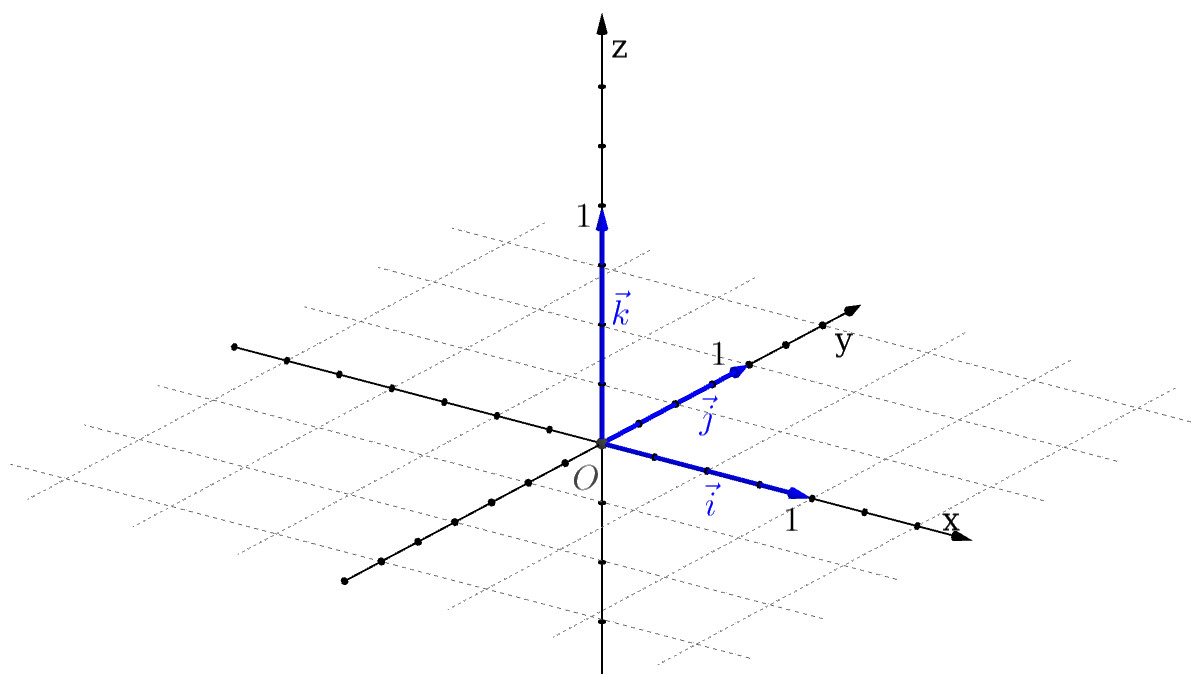
\includegraphics[width=5in]{./cap_base/dados/fig_base_ortonormal/fig.jpg}
  \caption{Representação gráfica de uma base ortonormal de vetores.}
  \label{cap_base_sec_base:fig:base_ortonormal}
\end{figure}

\begin{lema}\normalfont{(\hl{Pitágoras}{\pitagoras}.)}\label{cap_base_sec_base:lema:pitagoras}
  Se $\vec{u}\perp\vec{v}$, então 
  \begin{equation}
    \|\vec{u}+\vec{v}\|^2=\|\vec{u}\|^2+\|\vec{v}\|^2.
  \end{equation}
\end{lema}
\begin{demonstracao}
  Consulte o Exercício~\ref{cap_base_sec_base:exer:pitagoras}.
\end{demonstracao}

\begin{prop}\label{cap_base_sec_base:prop:norma}
  Seja $B = (\vec{i},\vec{j},\vec{k})$ uma base ortonormal e $\vec{u}=(u_1,u_2,u_3)_B$. Então, 
  \begin{equation}\hleq
    \|\vec{u}\|=\sqrt{u_1^2+u_2^2+u_3^2}.
  \end{equation}
\end{prop}
\begin{dem}
  Temos $\|\vec{u}\|^2 = \|u_1\vec{i}+u_2\vec{j}+u_3\vec{k}\|^2$. Seja $\pi$ um plano determinado por dadas representações de $\vec{i}$ e $\vec{j}$. Como $\vec{i}$, $\vec{j}$ e $\vec{k}$ são ortogonais, temos que $\vec{k}$ é ortogonal ao plano $\pi$. Além disso, o vetor $u_1\vec{i}+u_2\vec{j}$ também admite uma representação em $\pi$, logo $u_1\vec{i}+u_2\vec{j}$ é ortogonal a $\vec{k}$. Do Lema~\ref{cap_base_sec_base:lema:pitagoras}, temos
  \begin{equation}
    \|\vec{u}\|^2 = \|u_1\vec{i}+u_2\vec{j}\|^2 + \|u_3\vec{k}\|^2.
  \end{equation}
  Analogamente, como $u_1\vec{i}\perp u_2\vec{j}$, temos
  \begin{align}
    \|\vec{u}\|^2 &= \|u_1\vec{i}\|^2 + \|u_2\vec{j}\|^2 + \|u_3\vec{k}\|^2\\
                &= |u_1|^2\|\vec{i}\| + |u_2|^2\|\vec{j}\| + |u_3|\|\vec{k}\|^2\\
                &= u_1^2 + u_2^2 + u_3^2.
  \end{align}
  Extraindo a raiz quadrada de ambos os lados da última equação, obtemos o resultado desejado.
\end{dem}

A partir daqui, salvo dito o contrário, vamos assumir dada uma base ortonormal $B = (\vec{i}, \vec{j}, \vec{k})$ e, por simplicidade, escrevemos
\begin{align}
  \vec{u} &= (u_1, u_2, u_3)\\
          &= u_1\vec{i} + u_2\vec{j} + u_3\vec{k}.
\end{align}

\begin{ex}
  A norma de $\vec{u} = \left(-1,2,-\sqrt{2}\right)$, é
  \begin{align}
    \|\vec{u}\| &= \sqrt{(-1)^2 + 2^2 + \left(-\sqrt{2}\right)^2}\\
                &= \sqrt{7}.
  \end{align}
\end{ex}

\subsection{Exercícios Resolvidos}

\begin{exeresol}
  Considere a base $B=(\vec{i}, \vec{j}, \vec{k})$ ortonormal conforme dada na Figura~\ref{cap_base_sec_base:fig:base_ortonormal}. Faça uma representação do vetor 
  \begin{equation}
    \vec{u}=\left(2, \frac{1}{2}, 1\right)_B.
  \end{equation}
\end{exeresol}
\begin{resol}
  Primeiramente, observamos que
  \begin{align}
    \vec{u} &= \left(2, \frac{1}{2}, 1\right)_B\\
            &= 2\vec{i} + \frac{1}{2}\vec{j} + \vec{k}.
  \end{align}
  Assim sendo, podemos construir uma representação de $\vec{u}$ como dada na figura abaixo. Primeiramente, representamos os vetores $2\vec{i}$ e $\frac{1}{2}\vec{j}$ (cinza). Então, representamos o vetor $2\vec{i}+\frac{1}{2}\vec{j}$ (cinza). Por fim, temos a representação de $\vec{u}$ (vermelho).
  \begin{figure}[H]
    \centering
    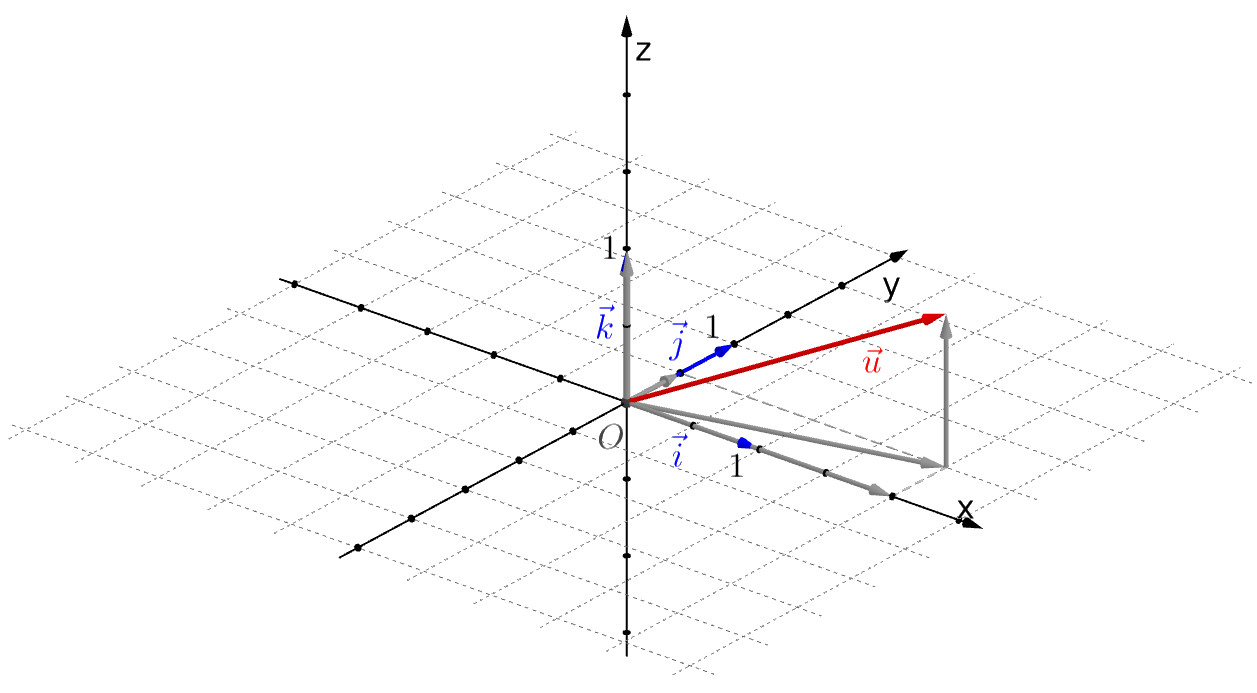
\includegraphics[width=5in]{cap_base/dados/fig_exeresol_base/fig.jpg}
  \end{figure}
\end{resol}

\begin{exeresol}
  Fixada uma base qualquer $B$ e dados $\vec{u}=(1,-1,2)_B$ e $\vec{v}=(-2,1,-1)_B$, encontre o vetor $\vec{x}$ que satisfaça
  \begin{equation}
    \vec{u}+2\vec{x}=\vec{v}-\left(\vec{x}+\vec{u}\right).
  \end{equation}
\end{exeresol}
\begin{resol}
  Primeiramente, podemos manipular a equação de forma a isolarmos $\vec{x}$ como segue
  \begin{gather}
    \vec{u}+2\vec{x}=\vec{v}-\left(\vec{x}+\vec{u}\right)\\
    2\vec{x}=-\vec{u}+\vec{v}-\vec{x}-\vec{u}\\
    3\vec{x}=\vec{v}-2\vec{u}\\
    \vec{x}=\frac{1}{3}\vec{v}-\frac{2}{3}\vec{u}
  \end{gather}
  Agora, sabendo que $\vec{u}=(1,-1,2)_B$ e $\vec{v}=(-2,1,-1)_B$, temos
  \begin{gather}
    \vec{x}=\frac{1}{3}(-2,1,-1)_B-\frac{2}{3}(1,-1,2)_B\\
    \vec{x}=\left(-\frac{2}{3},\frac{1}{3},-\frac{1}{3}\right)_B-\left(\frac{2}{3},-\frac{2}{3},\frac{4}{3}\right)_B\\
    \vec{x}=\left(-\frac{2}{3}-\frac{2}{3},\frac{1}{3}+\frac{2}{3},-\frac{1}{3}-\frac{4}{3}\right)\\
    \vec{x}=\left(-\frac{4}{3},1,-\frac{5}{3}\right)_B.
  \end{gather}
\end{resol}

\begin{exeresol}
  Fixada uma base $B$ qualquer, verifique se os vetores $\vec{u}=(1,-1,2)_B$, $\vec{v}=(-2,1,-1)_B$ e $\vec{w}=(-4,3,-5)$ também formam um base para o espaço de vetores.
\end{exeresol}
\begin{resol}
  Uma base para o espaço tridimensional $V$ é uma sequência de três vetores l.i.. Logo, para resolver a questão, basta verificar se $(\vec{u},\vec{v},\vec{w})$ é l.i.. Com base na Subseção \ref{cap_base_sec_base_subsec_dl}, basta calcularmos o determinante da matriz cujas colunas são formadas pelas coordenadas dos vetores da sequência, i.e.
  \begin{gather}
    \begin{vmatrix}
      u_1 & v_1 & w_1 \\
      u_2 & v_2 & w_2 \\
      u_3 & v_3 & w_3
    \end{vmatrix}\\
    = \begin{vmatrix}
      1 & -2 & -4 \\
      -1 & 1 & 3 \\
      2 & -1 & -5
    \end{vmatrix}\\
    = -5-4-12-(-8-3-10)\\
    = -21+21 = 0.
  \end{gather}
  Como este determinando é nulo, concluímos que $(\vec{u},\vec{v},\vec{w})$ é l.d. e, portanto, não forma uma base para $V$.
\end{resol}

\subsection{Exercícios}

\begin{exer}
  Considere a base $B=(\vec{i}, \vec{j}, \vec{k})$ conforme dada na Figura~\ref{cap_base_sec_base:fig:base_ortonormal}. Faça um esboço do vetor $\vec{u}=\left(1,-1,\frac{1}{2}\right)_B$.  
\end{exer}

\begin{exer}
  Fixada uma base $B=(\vec{i},\vec{j},\vec{k})$ e sabendo que $\vec{v}=(2, 0, -3)_B$, escreva $\vec{v}$ como combinação linear de $\vec{i}$, $\vec{j}$ e $\vec{k}$.
\end{exer}
\begin{resp}
  $\vec{v}=2\vec{i}+0\vec{j}-3\vec{k}$
\end{resp}

\begin{exer}
  Fixada uma base $B$ qualquer e $\vec{a}=\left(0,-1,1\right)_B$, $\vec{b}=\left(2,0,-1\right)_B$ e $\vec{c}=\left(\frac{1}{2},-\frac{1}{3},1\right)_B$, calcule:
  \begin{enumerate}[a)]
  \item $6\vec{c}$
  \item $-\vec{b}$
  \item $\vec{c}-\vec{b}$
  \item $2\vec{c}-(\vec{a}-\vec{b})$
  \end{enumerate}
\end{exer}
\begin{resp}
  a)~$6\vec{c}=(3,-2,6)_B$; b)~$-\vec{b}=(-2,0,1)_B$; c)~$\vec{c}-\vec{b}=(-\frac{3}{2},-\frac{1}{3},2)_B$; d)~$2\vec{c}-(\vec{a}-\vec{b})=(3,\frac{1}{3},0)_B$
\end{resp}

\begin{exer}
  Faxada uma base $B$ qualquer, verifique se os seguintes conjuntos de vetores são l.i. ou l.d..
  \begin{enumerate}[a)]
  \item $\vec{i}=(1,0,0)_B$, $\vec{j}=(0,1,0)_B$
  \item $\vec{a}=(1,2,0)_B$, $\vec{b}=(-2,-4,1)_B$
  \item $\vec{a}=(1,2,0)_B$, $\vec{c}=(-2,-4,0)_B$
  \item $\vec{i}=(1,0,0)_B$, $\vec{k}=(0,0,1)_B$
  \item $\vec{j}=(0,1,0)_B$, $\vec{k}=(0,0,1)_B$
  \item $\vec{a}=(1,2,-1)_B$, $\vec{d}=(\frac{1}{2},1,-\frac{1}{2})_B$
  \end{enumerate}
\end{exer}
\begin{resp}
  a)~l.i.; b)~l.i.; c)~l.d.; d)~l.i.; e)~l.i.; f)~l.d.
\end{resp}

\begin{exer}
  Faxada uma base $B$ qualquer, verifique se os seguintes conjuntos de vetores são l.i. ou l.d..
  \begin{enumerate}[a)]
  \item $\vec{i}=(1,0,0)_B$, $\vec{j}=(0,1,0)_B$, $\vec{k}=(0,0,1)_B$
  \item $\vec{a}=(0,-1,1)_B$, $\vec{b}=(2,0,-1)$, $\vec{c}=(\frac{1}{2},-\frac{1}{3},1)_B$
  \item $\vec{u}=(0,-1,1)_B$, $\vec{v}=(2,0,-1)$, $\vec{w}=(2,-1,0)_B$
  \end{enumerate}
\end{exer}
\begin{resp}
  a)~l.i.; b)~l.i.; c)~l.d.
\end{resp}

\begin{exer}
  Seja $B = (\vec{a}, \vec{b}, \vec{c})$ uma base ortogonal, i.e. $\vec{a}$, $\vec{b}$ e $\vec{c}$ são l.i. e dois a dois ortogonais. Mostre que $C = (\vec{a}/|\vec{a}|,\vec{b}/|\vec{b}|,\vec{c}/|\vec{c}|)$ é uma base ortonormal.
\end{exer}
\begin{resp}
  Segue imediatamente do fato de que $\left|\vec{u}/|u|\right|=1$ para qualquer vetor $\vec{u}\neq 0$.
\end{resp}

\begin{exer}\label{cap_base_sec_base:exer:pitagoras}
  Demostre o Lema~\ref{cap_base_sec_base:lema:pitagoras}.
\end{exer}
\begin{resp}

  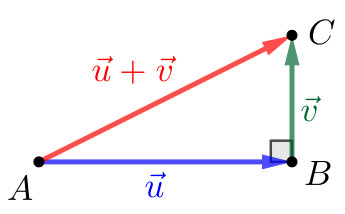
\includegraphics[width=2in]{./cap_base/dados/fig_pitagoras/fig.jpg}
  
  Sejam as representações $\vec{u}=\overrightarrow{AB}$, $\vec{v}=\overrightarrow{BC}$ e, portanto, $\vec{u}+\vec{v}=\overrightarrow{AC}$. Como $\vec{u}\perp\vec{v}$, temos que o triângulo $ABC$ é retângulo e, pelo Teorema de Pitágoras, segue que $\|\overrightarrow{AC}\|^2=\|\overrightarrow{AB}\|^2+\|\overrightarrow{BC}\|^2$. Logo, $\|\vec{u}+\vec{v}\|^2 = \|\vec{u}\|^2 + \|\vec{v}\|^2$.
\end{resp}

\ifisbook
\subsubsection{Respostas}
\shipoutAnswer
\fi

\section{Mudança de base}\label{cap_base_sec_mudbas}
\badgeRevisar

Sejam $B = (\vec{u}, \vec{v}, \vec{w})$ e $C = (\vec{r}, \vec{s}, \vec{t})$ bases do espaço $V$. Conhecendo as coordenadas de um vetor na base $C$, queremos determinar suas coordenadas na base $B$. Mais especificamente, seja
\begin{align}
  \vec{z} &= (z_1, z_2, z_3)_C\\
  &= z_1\vec{r} + z_2\vec{s} + z_3\vec{t}.
\end{align}
Agora, tendo $\vec{r} = (r_1, r_2, r_3)_B$, $\vec{s} = (s_1, s_2, s_3)_B$ e $\vec{t} = (t_1, t_2, t_3)_B$, então
\begin{align}
  (z_1, z_2, z_3)_C &= z_1(r_1, r_2, r_3)_B \\
                    &+ z_2(s_1, s_2, s_3)_B \\
                    &+ z_3(t_1, t_2, t_3)_B\\
                    &= \underbrace{(r_1z_1+s_1z_2+t_1z_3)}_{z_1'}\vec{u}\\
                    &+ \underbrace{(r_2z_1+s_2z_2+t_2z_3)}_{z_2'}\vec{v}\\
                    &+ \underbrace{(r_3z_1+s_3z_2+t_3z_3)}_{z_3'}\vec{w}
\end{align}
o que é equivalente a
\begin{equation}\label{eq:cbsmb_mcb}
  \begin{bmatrix}
    z_1'\\
    z_2'\\
    z_3'
  \end{bmatrix} =
  \underbrace{\begin{bmatrix}
    r_1 & s_1 & t_1\\
    r_2 & s_2 & t_2\\
    r_3 & s_3 & t_3
  \end{bmatrix}}_{M_{CB}}
  \begin{bmatrix}
    z_1\\
    z_2\\
    z_3
  \end{bmatrix},
\end{equation}
onde $\vec{z} = (z_1', z_2', z_3')_B$.

A matriz $M_{CB}$ é chamada de matriz de mudança de base de $C$ para $B$. Como os vetores $\vec{r}$, $\vec{s}$ e $\vec{t}$ são l.i., temos que a matriz de mudança de base $M_{BC}$ tem determinante não nulo e, portanto é invertível. Portanto, multiplicando por $M_{BC}^{-1}$ pela esquerda em \eqref{eq:cbsmb_mcb}, temos
\begin{equation}
    \begin{bmatrix}
    z_1\\
    z_2\\
    z_3
  \end{bmatrix} =
  \underbrace{\begin{bmatrix}
    r_1 & s_1 & t_1\\
    r_2 & s_2 & t_2\\
    r_3 & s_3 & t_3
  \end{bmatrix}^{-1}}_{M_{BC}}
  \begin{bmatrix}
    z_1'\\
    z_2'\\
    z_3'
  \end{bmatrix},
\end{equation}
ou seja
\begin{equation}
  M_{BC} = (M_{CB})^{-1}. 
\end{equation}

\begin{ex}
  Sejam dadas as bases $B = (\vec{a},\vec{b},\vec{c})$ e $C = (\vec{u},\vec{v},\vec{w})$, com $\vec{u}=(1,2,0)_B$, $\vec{v}=(2,0,-1)_B$ e $\vec{w}=(-1,-3,1)_B$. Seja, ainda, o vetor $\vec{z} = (1,-2,1)_B$. Vamos encontrar as coordenadas de $\vec{z}$ na base $C$.

  Há duas formas de proceder.

  {\bf Método 1.}
  
  A primeira consiste em resolver, de forma direta, a seguinte equação
  \begin{equation}
    (1,-2,1)_B = (x,y,z)_C.
  \end{equation}
  Esta é equivalente a
  \begin{align}
    \vec{a}-2\vec{b}+\vec{c} &= x\vec{u}+y\vec{v}+z\vec{w} \\
            &= x(1,2,0)_B \\
            &+ y(2,0,-1)_B\\
            &+ z(-1,-3,1)_B\\
            &= x(\vec{a}+2\vec{b})\\
            &+ y(2\vec{a}-\vec{c})\\
            &+ z(-\vec{a}-3\vec{b}+\vec{c})\\
            &= (x+2y-z)\vec{a}\\
            &+ (2x-3z)\vec{b}\\
            &+ (-y+z)\vec{c}
  \end{align}
  Isto nos leva ao seguinte sistema linear
  \begin{equation}
    \left\{
      \begin{array}{l}
        x+2y-z=1\\
        2x-3z=-2\\
        -y+z=1
      \end{array}
\right.
\end{equation}
Resolvendo este sistema, obtemos $x=7/5$, $y=3/5$ e $z=8/5$, i.e.
\begin{equation}
  \vec{z} = \left(\frac{7}{5},\frac{3}{5},\frac{8}{5}\right)_C.
\end{equation}

  {\bf Método 2.}

Outra maneira de se obter as coordenadas de $\vec{z}$ na base $C$ é usando a matriz de mudança de base. A matriz de mudança da base $C$ para a base $B$ é
\begin{align}
  M_{CB} &= \begin{bmatrix}
    u_1 & v_1 & w_1 \\
    u_2 & v_2 & w_2 \\
    u_3 & v_3 & w_3
  \end{bmatrix} \\
         &=
  \begin{bmatrix}
    1 & 2 & -1\\
    2 & 0 & -3\\
    0 & -1 & 1
  \end{bmatrix}.
\end{align}
Entretanto, neste exemplo, queremos fazer a mudança de $B$ para $C$. Portanto, calculamos a matriz de mudança de base $M_{BC}$. Segue:
\begin{gather}
  M_{BC} = M_{CB}^{-1} \\
  M_{BC} =
  \begin{bmatrix}
    1 & 2 & -1\\
    2 & 0 & -3\\
    0 & -1 & 1
  \end{bmatrix}^{-1} \\
  M_{BC} = 
  \begin{bmatrix}
    \frac{3}{5} & \frac{1}{5} & \frac{6}{5}\\
    \frac{2}{5} & -\frac{1}{5} & -\frac{1}{5}\\
    \frac{2}{5} & -\frac{1}{5} & \frac{4}{5}
  \end{bmatrix}
\end{gather}
Com esta matriz e denotando $\vec{z}=(x,y,z)_C$, temos
\begin{gather}
  \begin{bmatrix}
    x\\
    y\\
    z
  \end{bmatrix} = 
  \underbrace{\begin{bmatrix}
    \frac{3}{5} & \frac{1}{5} & \frac{6}{5}\\
    \frac{2}{5} & -\frac{1}{5} & -\frac{1}{5}\\
    \frac{2}{5} & -\frac{1}{5} & \frac{4}{5}
  \end{bmatrix}}_{M_{BC}}
  \begin{bmatrix}
    1\\
    -2\\
    1
  \end{bmatrix}\\
  \begin{bmatrix}
    x\\
    y\\
    z
  \end{bmatrix} =
    \begin{bmatrix}
    7/5\\
    3/5\\
    8/5
  \end{bmatrix}
\end{gather}
Logo, temos
\begin{equation}
  \vec{z} = \left(\frac{7}{5},\frac{3}{5},\frac{8}{5}\right)_C.
\end{equation}
\end{ex}

\subsection*{Exercícios resolvidos}

\begin{exeresol}\label{exeresol:cbsmb_mbccb}
  Sejam $B$ e $C$ bases dadas do espaço $V$. Sabendo que a matriz de mudança de base de $B$ para $C$ é
  \begin{equation}
    M =
    \begin{bmatrix}
      1 & 0 & -1 \\
      -1 & 1 & 0 \\
      2 & 3 & 1
    \end{bmatrix},
  \end{equation}
  calcule a matriz de mudança de base de $C$ para $B$.
\end{exeresol}
\begin{resol}
  Sejam $M_{BC}=M$ a matriz de mudança de base de $B$ para $C$ e $M_{CB}$ a matriz de mudança de base de $C$ para $B$. Temos
  \begin{gather}
    M_{CB} = M_{BC}^{-1}\\
    M_{CB} = M^{-1}\\
    M_{CB} =
    \begin{bmatrix}
      1 & 0 & -1 \\
      -1 & 1 & 0 \\
      2 & 3 & 1      
    \end{bmatrix}^{-1}\\
    M_{CB} =
    \begin{bmatrix}
      \frac{1}{6} & - \frac{1}{2} & \frac{1}{6}\\
      \frac{1}{6} & \frac{1}{2} & \frac{1}{6}\\
      - \frac{5}{6} & - \frac{1}{2} & \frac{1}{6}
    \end{bmatrix}
  \end{gather}
\end{resol}

\begin{exeresol}
  Fixadas as mesmas bases do ER \ref{exeresol:cbsmb_mbccb}, determine as coordenadas do vetor $\vec{u}$ na base $C$, sabendo que $\vec{u}=(2,-1,-3)_B$.
\end{exeresol}
\begin{resol}
  Denotando $\vec{u}=(u_1,u_2,u_3)_B$, temos
  \begin{gather}
    \vec{u}_C = M_{BC}\vec{u}_{B} \\
    \begin{bmatrix}
      u_1\\
      u_2\\
      u_3
    \end{bmatrix} =
    \begin{bmatrix}
      1 & 0 & -1 \\
      -1 & 1 & 0 \\
      2 & 3 & 1
    \end{bmatrix}
    \begin{bmatrix}
      2\\
      -1\\
      -3
    \end{bmatrix}\\
    \begin{bmatrix}
      u_1\\
      u_2\\
      u_3
    \end{bmatrix} =
    \begin{bmatrix}
      5\\
      -3\\
      -2
    \end{bmatrix}
  \end{gather}
\end{resol}

\begin{exeresol}
  Considere dadas as bases $A$, $B$ e $C$. Sejam, também, $M_{AB}$ a matriz de mudança de base de $A$ para $B$ e $M_{BC}$ a matriz de mudança de base de $B$ para $C$. Determine a matriz de mudança de base de $A$ para $C$ em função das matrizes $M_{AB}$ e $M_{BC}$.
\end{exeresol}
\begin{resol}
  Para um vetor $\vec{u}$ qualquer, temos
  \begin{gather}
    \vec{u}_B = M_{AB}\vec{u}_A\\
    \vec{u}_C = M_{BC}\vec{u}_B
  \end{gather}
  Logo, temos
  \begin{align}
    \vec{u}_C &= M_{BC}\left(M_{AB}\vec{u}_A\right)\\
              &= \left(M_{BC}M_{AB}\right)\vec{u}_A.
  \end{align}
  Concluímos que $M_{AC} = M_{BC}M_{AB}$.
\end{resol}

\subsection*{Exercícios}

\begin{exer}
  Sejam $A$ e $B$ bases dadas de $V$ (espaço tridimensional). Sabendo que $\vec{v}=(-2,0,1)_A$ e que a matriz de mudança de base
  \begin{equation}
    M_{AB} =
    \begin{matrix}
      1 & 0 & -1 \\
      0 & 2 & -1 \\
      -1 & 1 & 0
    \end{matrix},
  \end{equation}
  determine $\vec{v}_B$, i.e. as coordenadas de $\vec{v}$ na base $B$.
\end{exer}
\begin{resp}
  $\vec{v}=(-3,-1,2)_{B}$
\end{resp}

\begin{exer}
  Sejam $A$ e $B$ bases dadas de $V$ (espaço tridimensional). Sabendo que $\vec{v}=(-2,0,1)_B$ e que a matriz de mudança de base
  \begin{equation}
    M_{AB} =
    \begin{matrix}
      1 & 0 & -1 \\
      0 & 2 & -1 \\
      -1 & 1 & 0
    \end{matrix},
  \end{equation}
  determine $\vec{v}_A$, i.e. as coordenadas de $\vec{v}$ na base $A$.
\end{exer}
\begin{resp}
  $\vec{v}=(0,1,2)_{A}$
\end{resp}

\begin{exer}
  Sejam $B=(\vec{a},\vec{b},\vec{c})$ e $C=(\vec{u},\vec{v},\vec{w})$ bases de $V$ com
  \begin{gather}
    \vec{u} = (0,1,1)_B\\
    \vec{v} = (1,0,1)_B\\
    \vec{w} = (2,1,-1)_B
  \end{gather}
  Forneça a matriz de mudança de base $M_{CB}$.
\end{exer}
\begin{resp}
  $\displaystyle
  \begin{bmatrix}
    0 & 1 & 2\\
    1 & 0 & 1\\
    1 & 1 & -1
  \end{bmatrix}
$
\end{resp}

\begin{exer}
  Sejam $B=(\vec{a},\vec{b},\vec{c})$ e $C=(\vec{u},\vec{v},\vec{w})$ bases de $V$ com
  \begin{gather}
    \vec{a} = (0,1,1)_C\\
    \vec{b} = (1,0,1)_C\\
    \vec{c} = (2,1,-1)_C
  \end{gather}
  Forneça a matriz de mudança de base $M_{CB}$.
\end{exer}
\begin{resp}
  $\displaystyle
  \begin{bmatrix}
    - \frac{1}{4} & \frac{3}{4} & \frac{1}{4}\\
    \frac{1}{2} & - \frac{1}{2} & \frac{1}{2}\\
    \frac{1}{4} & \frac{1}{4} & - \frac{1}{4}
  \end{bmatrix}
$
\end{resp}

\begin{exer}
  Sejam $B=(\vec{a},\vec{b},\vec{c})$ e $C=(\vec{u},\vec{v},\vec{w})$ bases de $V$ com
  \begin{gather}
    \vec{u} = (0,1,1)_B\\
    \vec{v} = (1,0,1)_B\\
    \vec{w} = (2,1,-1)_B
  \end{gather}
  Sabendo que $\vec{d}=(0,-1,2)_{C}$, forneça $\vec{d}_B$, i.e. as coordenadas do vetor $\vec{d}$ na base $B$.
\end{exer}
\begin{resp}
  $\displaystyle\left[\begin{matrix}3\\2\\-3\end{matrix}\right]$
\end{resp}

\begin{exer}
  Sejam $B=(\vec{a},\vec{b},\vec{c})$ e $C=(\vec{u},\vec{v},\vec{w})$ bases de $V$ com
  \begin{gather}
    \vec{u} = (0,1,1)_B\\
    \vec{v} = (1,0,1)_B\\
    \vec{w} = (2,1,-1)_B
  \end{gather}
  Sabendo que $\vec{d}=(1,-2,1)_{B}$, forneça $\vec{d}_C$, i.e. as coordenadas do vetor $\vec{d}$ na base $C$.
\end{exer}
\begin{resp}
  $\displaystyle\left[\begin{matrix}- \frac{3}{2}\\2\\- \frac{1}{2}\end{matrix}\right]$
\end{resp}

\begin{exer}
  Considere dadas as bases $A$, $B$ e $C$ do espaço tridimensional $V$. Sejam, também, $M_{AB}$ a matriz de mudança de base de $A$ para $B$ e $M_{CB}$ a matriz de mudança de base de $C$ para $B$. Determine a matriz de mudança de base de $A$ para $C$ em função das matrizes $M_{AB}$ e $M_{CB}$.  
\end{exer}
\begin{resp}
  $M_{AC}=M_{CB}^{-1}M_{AB}$
\end{resp}
%Este trabalho está licenciado sob a Licença Atribuição-CompartilhaIgual 4.0 Internacional Creative Commons. Para visualizar uma cópia desta licença, visite http://creativecommons.org/licenses/by-sa/4.0/deed.pt_BR ou mande uma carta para Creative Commons, PO Box 1866, Mountain View, CA 94042, USA.

\chapter{Produtos}\label{cap_produtos}
\badgeRevisar

\section{Produto Escalar}\label{cap_produtos_sec_prodesc}
\badgeRevisar

Ao longo desta seção, assumiremos $B = (\vec{i},\vec{j},\vec{k})$ uma base ortonormal no espaço\footnote{$(\vec{i},\vec{j},\vec{k})$ é l.i., $|\vec{i}|=1$, $|\vec{j}|=1$, $|\vec{k}|=1$ e dois a dois ortogonais. Veja Subseção \ref{subsec:cbsbc_bortonormal}.}. Por simplicidade de notação, vamos denotar as coordenas de um vetor $\vec{u}$ na base $B$ por
\begin{equation}
  \vec{u} = (u_1, u_2, u_3),
\end{equation}
i.e. $\vec{u} = u_1\vec{i} + u_2\vec{j} + u_3\vec{k}$.

O {\color{blue}\bf produto escalar} dos vetores $\vec{u} = (u_1,u_2,u_3)$ e $\vec{v}=(v_1,v_2,v_3)$ é o número real
\begin{equation}\label{eq:prodesc_ortonormal}
  {\color{blue}\vec{u}\cdot\vec{v} = u_1v_1+u_2v_2+u_3v_3}.
\end{equation}

\begin{ex}
  Se $\vec{u}=(2,-1,3)$ e $\vec{v}=(-3,-4,2)$, então
  \begin{equation}
    \vec{u}\cdot\vec{v} = 2\cdot(-3)+(-1)\cdot(-4)+3\cdot 2 = 4.
  \end{equation}
\end{ex}

\subsection{Propriedades do Produto Escalar}

Quaisquer que sejam $\vec{u}$, $\vec{v}$, $\vec{w}$ e qualquer número real $\alpha$, temos:
\begin{itemize}
\item {\bf Comutatividade:}
  \begin{equation}
    {\color{blue}\vec{u}\cdot\vec{v}=\vec{v}\cdot\vec{u}}
  \end{equation}

  Dem.:
  \begin{align}
    \vec{u}\cdot\vec{v} &= (u_1,u_2,u_3)\cdot(v_1,v_2,v_3)\\
                        &= u_1v_1+u_2v_2+u_3v_3 \\
                        &= v_1u_1+v_2u_2+v_3u_3 \\
                        &= \vec{v}\cdot\vec{u}.
  \end{align}

\item {\bf Associatividade com a multiplicação por escalar:}
  \begin{equation}
    {\color{blue}(\alpha\vec{u})\cdot\vec{v}=\vec{u}\cdot(\alpha\vec{v})=\alpha(\vec{u}\cdot\vec{v})}
\end{equation}

  Dem.:
  \begin{align}
    (\alpha\vec{u})\cdot\vec{v} &= (\alpha u_1,\alpha u_2, \alpha u_3)\cdot (v_1,v_2,v_3)\\
                                &= (\alpha u_1)v_1+(\alpha u_2)v_2 + (\alpha u_3)v_3 \\
                                &= \alpha (u_1v_1)+\alpha (u_2v_2)+\alpha (u_3v_3) \\
                                &= \alpha (u_1v_1+u_2v_2+u_3v_3) = \alpha(\vec{u}\cdot\vec{v})\\
                                &= u_1(\alpha v_1) + u_2(\alpha v_2) + u_3(\alpha v_3) \\
                                &= (u_1,u_2,u_3)\cdot(\alpha v_1,\alpha v_2,\alpha v_3) \\
                                &= \vec{u}\cdot(\alpha\vec{v}).
  \end{align}

\item {\bf Distributividade com a adição:}
  \begin{equation}
    {\color{blue}\vec{u}\cdot(\vec{v}+\vec{w}) = \vec{u}\cdot\vec{v}+\vec{u}\cdot\vec{w}}
\end{equation}
  Dem.:
  \begin{align}
    \vec{u}\cdot(\vec{v}+\vec{w}) &= (u_1,u_2,u_3)\cdot\left((v_1,v_2,v_3)+(w_1,w_2,w_3)\right) \\
                                  &= (u_1,u_2,u_3)\cdot [(v_1+w_1,v_2+w_2,v_3+w_3)] \\
                                  &= u_1(v_1+w_1) + u_2(v_2+w_2) + u_2(v_2+w_2) \\
                                  &= u_1v_1+u_1w_1+u_2v_2+u_2w_2+u_3v_3+u_3w_3 \\
                                  &= u_1v_1+u_2v_2+u_3v_3 + u_1w_1+u_2w_2+u_3w_3 \\
                                  &= \vec{u}\cdot\vec{v}+\vec{u}\cdot\vec{w}.
  \end{align}

\item {\bf Sinal:}
  \begin{gather}
    {\color{blue}\vec{u}\cdot\vec{u}\geq 0},\quad\text{e}\\
    {\color{blue}\vec{u}\cdot\vec{u}=0 \Leftrightarrow \vec{u}=\vec{0}}
\end{gather}

  Dem.:
  \begin{align}
    \vec{u}\cdot\vec{u} = u_1^2+u_2^2+u_3^2 \geq 0.
  \end{align}
  Além disso, observamos que a soma de números não negativos é nula se, e somente se, os números forem zeros.

\item {\bf Norma:}
  \begin{equation}
    {\color{blue}|u|^2 = \vec{u}\cdot\vec{u}}
\end{equation}
  Dem.:
  Como fixamos uma base ortonormal $B$, a Proposição \ref{prop:bo_norma} nos garante que
  \begin{equation}
    |u|^2 = u_1^2+u_2^2+u_3^2 = \vec{u}\cdot\vec{u}.
  \end{equation}
\end{itemize}

\begin{ex}
  Sejam $\vec{u}=(-1,2,1)$, $\vec{v}=(2,-1,3)$ e $\vec{w}=(1,0,-1)$. Vejamos se as propriedades se verificam para estes vetores.
  \begin{itemize}
  \item Comutatividade:
    \begin{gather}
      \vec{u}\cdot\vec{v} = -1\cdot 2 + 2\cdot (-1) + 1\cdot 3 = -1\\
      \vec{v}\cdot\vec{u} = 2\cdot(-1) + (-1)\cdot 2 + 3\cdot 1 = -1~\checkmark
    \end{gather}
  \item Associatividade com a multiplicação por escalar:
    \begin{gather}
      (2\vec{u})\cdot\vec{v} = (-2,4,2)\cdot(2,-1,3) = -4-4+6=-2\\
      2(\vec{u}\cdot\vec{v}) = 2(-2-2+3) = -2~\checkmark\\
      \vec{u}\cdot(2\vec{v}) = (-1,2,1)\cdot(4,-2,6) = -2~\checkmark
    \end{gather}
  \item Distributividade com a adição:
    \begin{gather}
      \vec{u}\cdot(\vec{v}+\vec{w}) = (-1,2,1)\cdot(3,-1,2) = -3-2+2=-3\\
      \vec{u}\cdot\vec{v}+\vec{u}\cdot\vec{w} = (-2-2+3)+(-1+0-1) = -3~\checkmark
    \end{gather}
  \item Sinal:
    \begin{equation}
      \vec{w}\cdot\vec{w} = 1+0+1 = 2 \geq 0~\checkmark
    \end{equation}
  \item Norma:
    \begin{gather}
      |u|^2 = (-1)^2+2^2+1^2 = 6\\
      \vec{u}\cdot\vec{u} = (-1)\cdot(-1)+2\cdot 2+1\cdot 1 = 6~\checkmark
    \end{gather}
  \end{itemize}
\end{ex}

\subsection{Exercícios Resolvidos}

\begin{exeresol}
  Sejam
  \begin{gather}
    \vec{u} = (-1,0,1)\\
    \vec{v} = (0,2,1)\\
    \vec{w} = (2,-1,-1)
  \end{gather}
  calcule $\vec{w}\cdot\left(2\vec{u}-\vec{w}\right)-2\vec{u}\cdot\vec{w}$.
\end{exeresol}
\begin{resol}
  Vamos começar calculando o último termo.
  \begin{gather}
    \vec{w}\cdot\left(2\vec{u}-\vec{w}\right)-2\vec{u}\cdot\vec{w}\\
    = \vec{w}\cdot\left(2\vec{u}-\vec{w}\right)-2(-1,0,1)\cdot(2,-1,-1)
  \end{gather}
  Calculamos $2(-1,0,1)=(-2,0,2)$, logo, temos
  \begin{gather}
    \vec{w}\cdot\left(2\vec{u}-\vec{w}\right)-(-2,0,2)\cdot(2,-1,-1)\\
    = \vec{w}\cdot\left(2\vec{u}-\vec{w}\right)-(-2\cdot 2 + 0\cdot(-1)+2\cdot(-1))\\
    = \vec{w}\cdot\left(2\vec{u}-\vec{w}\right)-(-4-2)
  \end{gather}
  Agora, para o primeiro termo, podemos usar a propriedade distributiva, como segue
  \begin{gather}
    2\vec{w}\cdot\vec{u} - \vec{w}\cdot\vec{w}+6\\
    = 2(2,-1,-1)\cdot(-1,0,1) - |\vec{w}|^2+6\\
    = 2(-2+0-1)-(2^2+(-1)^2+(-1)^2)+6\\
    = -6 - 6 + 6 \\
    = -6
  \end{gather}
  Com isso, concluímos que $\vec{w}\cdot\left(2\vec{u}-\vec{w}\right)-2\vec{u}\cdot\vec{w} = -6$.
\end{resol}

\begin{exeresol}
  Sendo $B=(\vec{i},\vec{j},\vec{k})$ uma base ortonormal, mostre que o produto interno entre vetores distintos de $B$ é igual a zero. Ainda, o produto interno de um vetor de $B$ por ele mesmo é igual a 1.
\end{exeresol}
\begin{resol}
  Calculamos o produto interno entre vetores diferentes:
  \begin{align}
    \vec{i}\cdot\vec{j} &= (1,0,0)\cdot (0,1,0)\\
                        &= 1\cdot 0 + 0\cdot 1 + 0\cdot 0 \\
                        &= 0~\checkmark\\
                        &= \vec{j}\cdot\vec{i}
  \end{align}
  \begin{align}
    \vec{i}\cdot\vec{k} &= (1,0,0)\cdot (0,0,1)\\
                        &= 1\cdot 0 + 0\cdot 0 + 0\cdot 1 \\
                        &= 0~\checkmark \\
                        &= \vec{k}\cdot\vec{i}
  \end{align}
  \begin{align}
    \vec{j}\cdot\vec{k} &= (1,0,0)\cdot (0,0,1)\\
                        &= 1\cdot 0 + 0\cdot 0 + 0\cdot 1 \\
                        &= 0~\checkmark \\
                        &= \vec{k}\cdot\vec{j}
  \end{align}
  Por fim, verificamos os casos do produto interno de um vetor por ele mesmo:
  \begin{gather}
    \vec{i}\cdot\vec{i} = 1^2+0^2+0^2 = 1~\checkmark\\
    \vec{j}\cdot\vec{j} = 0^2+1^2+0^2 = 1~\checkmark\\
    \vec{k}\cdot\vec{k} = 0^2+0^2+1^2 = 1~\checkmark
  \end{gather}
\end{resol}

\subsection{Exercícios}

\begin{exer}
  Sendo $\vec{u}=(2,-1,1)$ e $\vec{v}=(1,-3,2)$, calcule:
  \begin{enumerate}[a)]
  \item $\vec{u}\cdot\vec{v}$
  \item $\vec{v}\cdot\vec{u}$
  \item $2\vec{u}\cdot\vec{v}$
  \item $\vec{u}\cdot(2\vec{v})$
  \end{enumerate}
\end{exer}
\begin{resp}
  a)~$7$; b)~$7$; c)~$14$; d)~$14$
\end{resp}

\begin{exer}
  Sendo $\vec{u}=(2,-1,1)$, calcule:
  \begin{enumerate}[a)]
  \item $\vec{u}\cdot\vec{i}$
  \item $\vec{u}\cdot\vec{j}$
  \item $2\vec{u}\cdot\vec{k}$
  \end{enumerate}
\end{exer}
\begin{resp}
  a)~$2$; b)~$-1$; c)~$2$
\end{resp}

\begin{exer}
  Sendo $\vec{u}=(2,-1,1)$, $\vec{v}=(1,-3,2)$ e $\vec{w}=(-2,-1,-3)$, calcule:
  \begin{enumerate}[a)]
  \item $\vec{u}\cdot(\vec{w}+\vec{v})$
  \item $\vec{v}\cdot(\vec{v}-2\vec{u})$
  \end{enumerate}
\end{exer}
\begin{resp}
  a)~$1$; b)~$0$;
\end{resp}

\begin{exer}
  Sendo $\vec{u}=(2,-1,1)$, $\vec{v}=(1,-3,2)$ e $\vec{w}=(-2,-1,-3)$, calcule:
  \begin{enumerate}[a)]
  \item $|\vec{u}|$
  \item $|\vec{u}+\vec{v}|$
  \item $|\vec{u}\cdot\vec{w}|$
  \end{enumerate}
\end{exer}
\begin{resp}
  a)~$\sqrt{6}$; b)~$\sqrt{34}$; c)~$6$;
\end{resp}

\begin{exer}
  Sendo $\vec{u}=(2,-1,1)$, $\vec{v}=(1,-3,2)$ e $\vec{w}=(-2,-1,-3)$, encontre o vetor $\vec{x}$ que satisfaz as seguintes condições:
  \begin{align}
    &\vec{u}\cdot\vec{x} = -1\\
    &\vec{v}\cdot\vec{x} = 2\\
    &\vec{w}\cdot\vec{x} = -4\\
  \end{align}
\end{exer}
\begin{resp}
  $x = (-23/16, 5/16, 35/16)$
\end{resp}

\begin{exer}
  Sendo $\vec{u}=(2,-1,1)$ e $\vec{v}=(1,-3,2)$, encontre o vetor $\vec{x}$ que satisfaz as seguintes condições:
  \begin{align}
    &\vec{u}\cdot\vec{x} = 0\\
    &\vec{v}\cdot\vec{x} = 0
  \end{align}
\end{exer}
\begin{resp}
  $\displaystyle x = \left(-\frac{1}{5}x_3, \frac{3}{5}x_3, x_3\right), x_3\in\mathbb{R}$
\end{resp}

\begin{exer}
  Sendo $\vec{u}=(2,-1,1)$, $\vec{v}=(1,-3,2)$ e $\vec{w}=(-2,-1,-3)$, encontre o vetor $\vec{x}$ que satisfaz as seguintes condições:
  \begin{align}
    &\vec{u}\cdot\vec{x} = 0\\
    &\vec{v}\cdot\vec{x} = 0\\
    &\vec{w}\cdot\vec{x} = 0\\
  \end{align}
\end{exer}
\begin{resp}
  $x = \vec{0}$
\end{resp}

\section{Ângulo entre Vetores}\label{cap_produtos_sec_angulo}
\badgeRevisar

O {\bf ângulo formado entre dois vetores} $\vec{u}$ e $\vec{v}$ não nulos, é definido como o menor ângulo determinado entre quaisquer representações $\vec{u} = \overrightarrow{OA}$ e $\vec{v} = \overrightarrow{OB}$.

\begin{figure}[H]
  \centering
  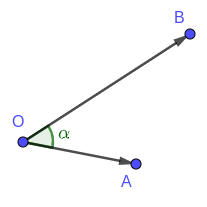
\includegraphics[width=0.4\textwidth]{./cap_produtos/dados/fig_vetangulo/fig_vetangulo}
  \caption{Ângulo entre dois vetores.}
  \label{fig:prodesc_vetangulo}
\end{figure}

\begin{prop}\label{prop:angulo_prodesc}
  Dados $\vec{u}$ e $\vec{v}$, temos
  \begin{equation}\label{eq:prodesc_eq}
    {\color{blue}\vec{u}\cdot\vec{v}=|\vec{u}||\vec{v}|\cos\alpha},
  \end{equation}
  onde $\alpha$ é o ângulo entre os vetores $\vec{u}$ e $\vec{v}$.
\end{prop}
\begin{dem}
  Tomamos as representações $\vec{u} = \overrightarrow{OA}$ e $\vec{v} = \overrightarrow{OB}$. Observamos que $\vec{u}-\vec{v} = \overrightarrow{BA}$. Então, aplicando a lei dos cossenos no triângulo $\triangle OAB$, obtemos
  \begin{equation}
    |\overrightarrow{BA}|^2 = |\overrightarrow{OA}|^2 + |\overrightarrow{OB}|^2 - 2|\overrightarrow{OA}||\overrightarrow{OB}|\cos\alpha,
  \end{equation}
  ou, equivalentemente,
  \begin{align}
    |\vec{u}-\vec{v}|^2 &= |\vec{u}|^2+|\vec{v}|^2-2|\vec{u}||\vec{v}|\cos\alpha\\
    (\vec{u}-\vec{v})\cdot(\vec{u}-\vec{v}) &= |\vec{u}|^2+|\vec{v}|^2-2|\vec{u}||\vec{v}|\cos\alpha\\
    \vec{u}\cdot\vec{u}-2\vec{u}\cdot\vec{v}+\vec{v}\cdot\vec{v} &= |\vec{u}|^2+|\vec{v}|^2-2|\vec{u}||\vec{v}|\cos\alpha\\
    |\vec{u}|^2+|\vec{v}|^2-2\vec{u}\cdot\vec{v} &= |\vec{u}|^2+|\vec{v}|^2-2|\vec{u}||\vec{v}|\cos\alpha
  \end{align}
  donde
  \begin{equation}
    \vec{u}\cdot\vec{v} = |\vec{u}||\vec{v}|\cos\alpha.
  \end{equation}
\end{dem}

\begin{ex}
  Vamos determinar ângulo entre os vetores $\displaystyle \vec{u}=\left(\frac{\sqrt{3}}{2},\frac{1}{2},0\right)$ e $\displaystyle \vec{u}=\left(\frac{1}{2},\frac{\sqrt{3}}{2},0\right)$. Da Proposição \ref{prop:angulo_prodesc}, temos
  \begin{gather}
    {\color{blue}\cos\alpha = \frac{\vec{u}\cdot\vec{v}}{|u|\cdot|v|}}\\
    \cos\alpha = \frac{\frac{\sqrt{3}}{2}\frac{1}{2}+\frac{1}{2}\frac{\sqrt{3}}{2}}{\sqrt{\left(\frac{\sqrt{3}}{2}\right)^2+\left(\frac{1}{2}\right)^2+0^2}\cdot \sqrt{\left(\frac{1}{2}\right)^2+\left(\frac{\sqrt{3}}{2}\right)^2+0^2}}\\
    \cos\alpha = \frac{\frac{\sqrt{3}}{2}}{1\cdot 1} = \frac{\sqrt{3}}{2}.
  \end{gather}
  Portanto, temos $\alpha = \pi/6$.
\end{ex}

\begin{obs}
  O {\bf ângulo} entre dois vetores $\vec{u}$ e $\vec{v}$ é:
  \begin{itemize}
  \item {\bf agudo} se, e somente se, $\vec{u}\cdot\vec{v} > 0$;
  \item {\bf obtuso} se, e somente se, $\vec{u}\cdot\vec{v} < 0$.
  \end{itemize}

  De fato, de \eqref{eq:prodesc_eq}, temos que o sinal de $\vec{u}\cdot\vec{v}$ é igual ao sinal de $\cos\alpha$ (o cosseno do ângulo entre os vetores). Também, por definição, $0 \leq \alpha \leq \pi$. Logo, se $\cos\alpha > 0$, então $0< \alpha < \pi/2$ (ângulo agudo) e, se $\cos\alpha < 0$, então $\pi/2 < \alpha < \pi$ (ângulo obtuso).
\end{obs}

\begin{obs}(Vetores ortogonais) 
  Se $\vec{u},\vec{v}\neq\vec{0}$, então:
  \begin{itemize}
  \item $\vec{u}\perp\vec{v}$ se, e somente se, $\vec{u}\cdot\vec{v}=0$.
  \end{itemize}

  De fato, seja $\alpha$ o ângulo entre $\vec{u}$ e $\vec{v}$. Se $\vec{u}\perp\vec{v}$, então $\alpha = \pi/2$ e
  \begin{align}
    \vec{u}\cdot\vec{v} &= |\vec{u}||\vec{v}|\cos\alpha\\
                        &= |\vec{u}||\vec{v}|\cos\left(\frac{\pi}{2}\right)\\
                        &= |\vec{u}|\cdot |\vec{v}|\cdot 0 \\
                        &= 0.
  \end{align}
  Reciprocamente, se $\vec{u}\cdot\vec{v} = 0$, então
  \begin{align}
    \cos\alpha &= \frac{\vec{u}\cdot\vec{v}}{|\vec{u}||\vec{v}|}\\
               &= \frac{0}{|\vec{u}||\vec{v}|} \\
               &= 0.
  \end{align}
  Lembrando que $0\leq \alpha\leq \pi$, segue que $\alpha = \pi/2$, i.e. $\vec{u}\perp\vec{v}$.
\end{obs}

\begin{ex}
  Os vetores $\vec{i}=(1,0,0)$ e $\vec{u}=(0,1,1)$ são ortogonais. De fato, temos
  \begin{align}
    \vec{i}\cdot\vec{j} &= 1\cdot 0 + 0\cdot 1 + 0\cdot 1 \\
                        &= 0.
  \end{align}
\end{ex}

\subsection{Desigualdade Triangular}

Dados dois vetores $\vec{u}$ e $\vec{v}$ temos
\begin{equation}
  {\color{blue}|\vec{u}+\vec{v}| \leq |\vec{u}| + |\vec{v}|},
\end{equation}
esta é conhecida como a {\bf desigualdade triangular}. Para demonstrá-la, começamos observando que
\begin{align}
  |\vec{u}+\vec{v}|^2 &= (\vec{u}+\vec{v})\cdot(\vec{u}+\vec{v})\\
                      &= \vec{u}\cdot\vec{v}+\vec{v}\cdot\vec{v}+\vec{u}\cdot\vec{v}+\vec{v}\cdot\vec{u}\\
                      &= |\vec{u}|^2 + |\vec{v}|^2 + 2\vec{u}\cdot\vec{v}.  
\end{align}
Agora, vamos estimar $\vec{u}\cdot\vec{v}$. Pela Proposição \ref{prop:angulo_prodesc}, temos
\begin{equation}
  \vec{u}\cdot\vec{v} = |\vec{u}||\vec{v}|\cos\alpha,
\end{equation}
onde $\alpha$ é o ângulo entre $\vec{u}$ e $\vec{v}$. Mas, então:
\begin{equation}
  \vec{u}\cdot\vec{v} \leq |\vec{u}||\vec{v}||\cos\alpha|.
\end{equation}
Daí, como $|\cos\alpha|\leq 1$, temos
\begin{equation}
  {\color{blue}\vec{u}\cdot\vec{v}\leq |\vec{u}||\vec{v}|},
\end{equation}
a qual é chamada de {\bf desigualdade de Cauchy-Schwarz}\footnote{Augustin-Louis Cauchy, 1798-1857, matemático francês. Fonte: \href{https://en.wikipedia.org/wiki/Augustin-Louis_Cauchy}{Wikipeida}. Hermann Schwarz, 1843-1921, matemático alemão. Fonte: \href{https://en.wikipedia.org/wiki/Hermann\_Schwarz}{Wikipedia}.}.

\subsection{Exercícios Resolvidos}

\begin{exeresol}
  Sejam $\vec{u}=(x,-1,2)$ e $\vec{v}=(2,x,-3)$. Determine $x$ tal que
  \begin{equation}
    \vec{u}\cdot\vec{v}=\frac{1}{2}.
  \end{equation}
\end{exeresol}
\begin{resol}
  Da definição do produto escalar, temos
  \begin{gather}
    \vec{u}\cdot\vec{v} = u_1v_1 + u_2v_2 + u_3v_3 \\
    \frac{1}{2} = 2x - x - 6 \\
    x - 6 = \frac{1}{2} \\
    x = \frac{1}{2} + 6 \\
    x = \frac{13}{2}.
  \end{gather}
\end{resol}

\begin{exeresol}
  Determine $x$ tal que $\vec{u}=(-1,0,x)$ seja ortogonal a $\vec{v}=(1,2,-1)$.
\end{exeresol}
\begin{resol}
  Para que $\vec{u}\perp\vec{v}$ devemos ter
  \begin{gather}
    \vec{u}\cdot\vec{v} = 0 \\
    -1 + 0 -x = 0 \\
    x = -1.
  \end{gather}
\end{resol}

\subsection{Exercícios}

\begin{exer}
  Determine o ângulo entre os vetores $\vec{u}=(1,0,1)$ e $\vec{v}=(0,0,2)$.
\end{exer}
\begin{resp}
  $\pi/4$
\end{resp}

\begin{exer}
  Seja $\vec{v} = (1,2,-1)$. Determine a norma do vetor $\vec{u}$ de mesma direção de $\vec{v}$ e tal que $\vec{u}\cdot\vec{v}=2$.
\end{exer}
\begin{resp}
  $\frac{\sqrt{6}}{3}$
\end{resp}

\begin{exer}
  Se $\vec{u}$ e $\vec{v}$ são vetores unitários e $\vec{u}\cdot\vec{v}=1$, então $\vec{u}$ e $\vec{v}$ têm a mesma direção e o mesmo sentido? Justifique sua resposta.
\end{exer}
\begin{resp}
  Sim.
\end{resp}

\begin{exer}
  Se $\vec{u}$ e $\vec{v}$ são vetores tais que $\vec{u}\cdot\vec{v}=-1$, então $\vec{u}$ e $\vec{v}$ têm a mesma direção e sentidos opostos? Justifique sua resposta.
\end{exer}
\begin{resp}
  Não necessariamente.
\end{resp}

\begin{exer}
  Encontre o vetor $x$ ortogonal a $\vec{u}=(1,-2,0)$ e $\vec{v}=(2,-1,1)$ tal que $\vec{x}\cdot(0,-1,2)=1$.
\end{exer}
\begin{resp}
  $\vec{x}=(-2/7,-1/7,3/7)$
\end{resp}

\section{Projeção Ortogonal}\label{cap_produtos_sec_proj}
\badgeRevisar

Sejam dados os vetores $\vec{u}=\overrightarrow{OA}$, $\vec{v}=\overrightarrow{OB}\neq\vec{0}$. Seja, ainda, $P$ a interseção da reta perpendicular a $OB$ que passa pelo ponto $A$. Observemos a Figura \ref{fig:proj}. Com isso, definimos a {\bf projeção ortogonal de $\vec{u}$ na direção de $\vec{v}$}  por $\overrightarrow{OP}$. Denotamos
\begin{equation}
  {\color{blue}\overrightarrow{OP} = \proj_{\vec{v}}\vec{u}}.
\end{equation}

\begin{figure}[H]
  \centering
  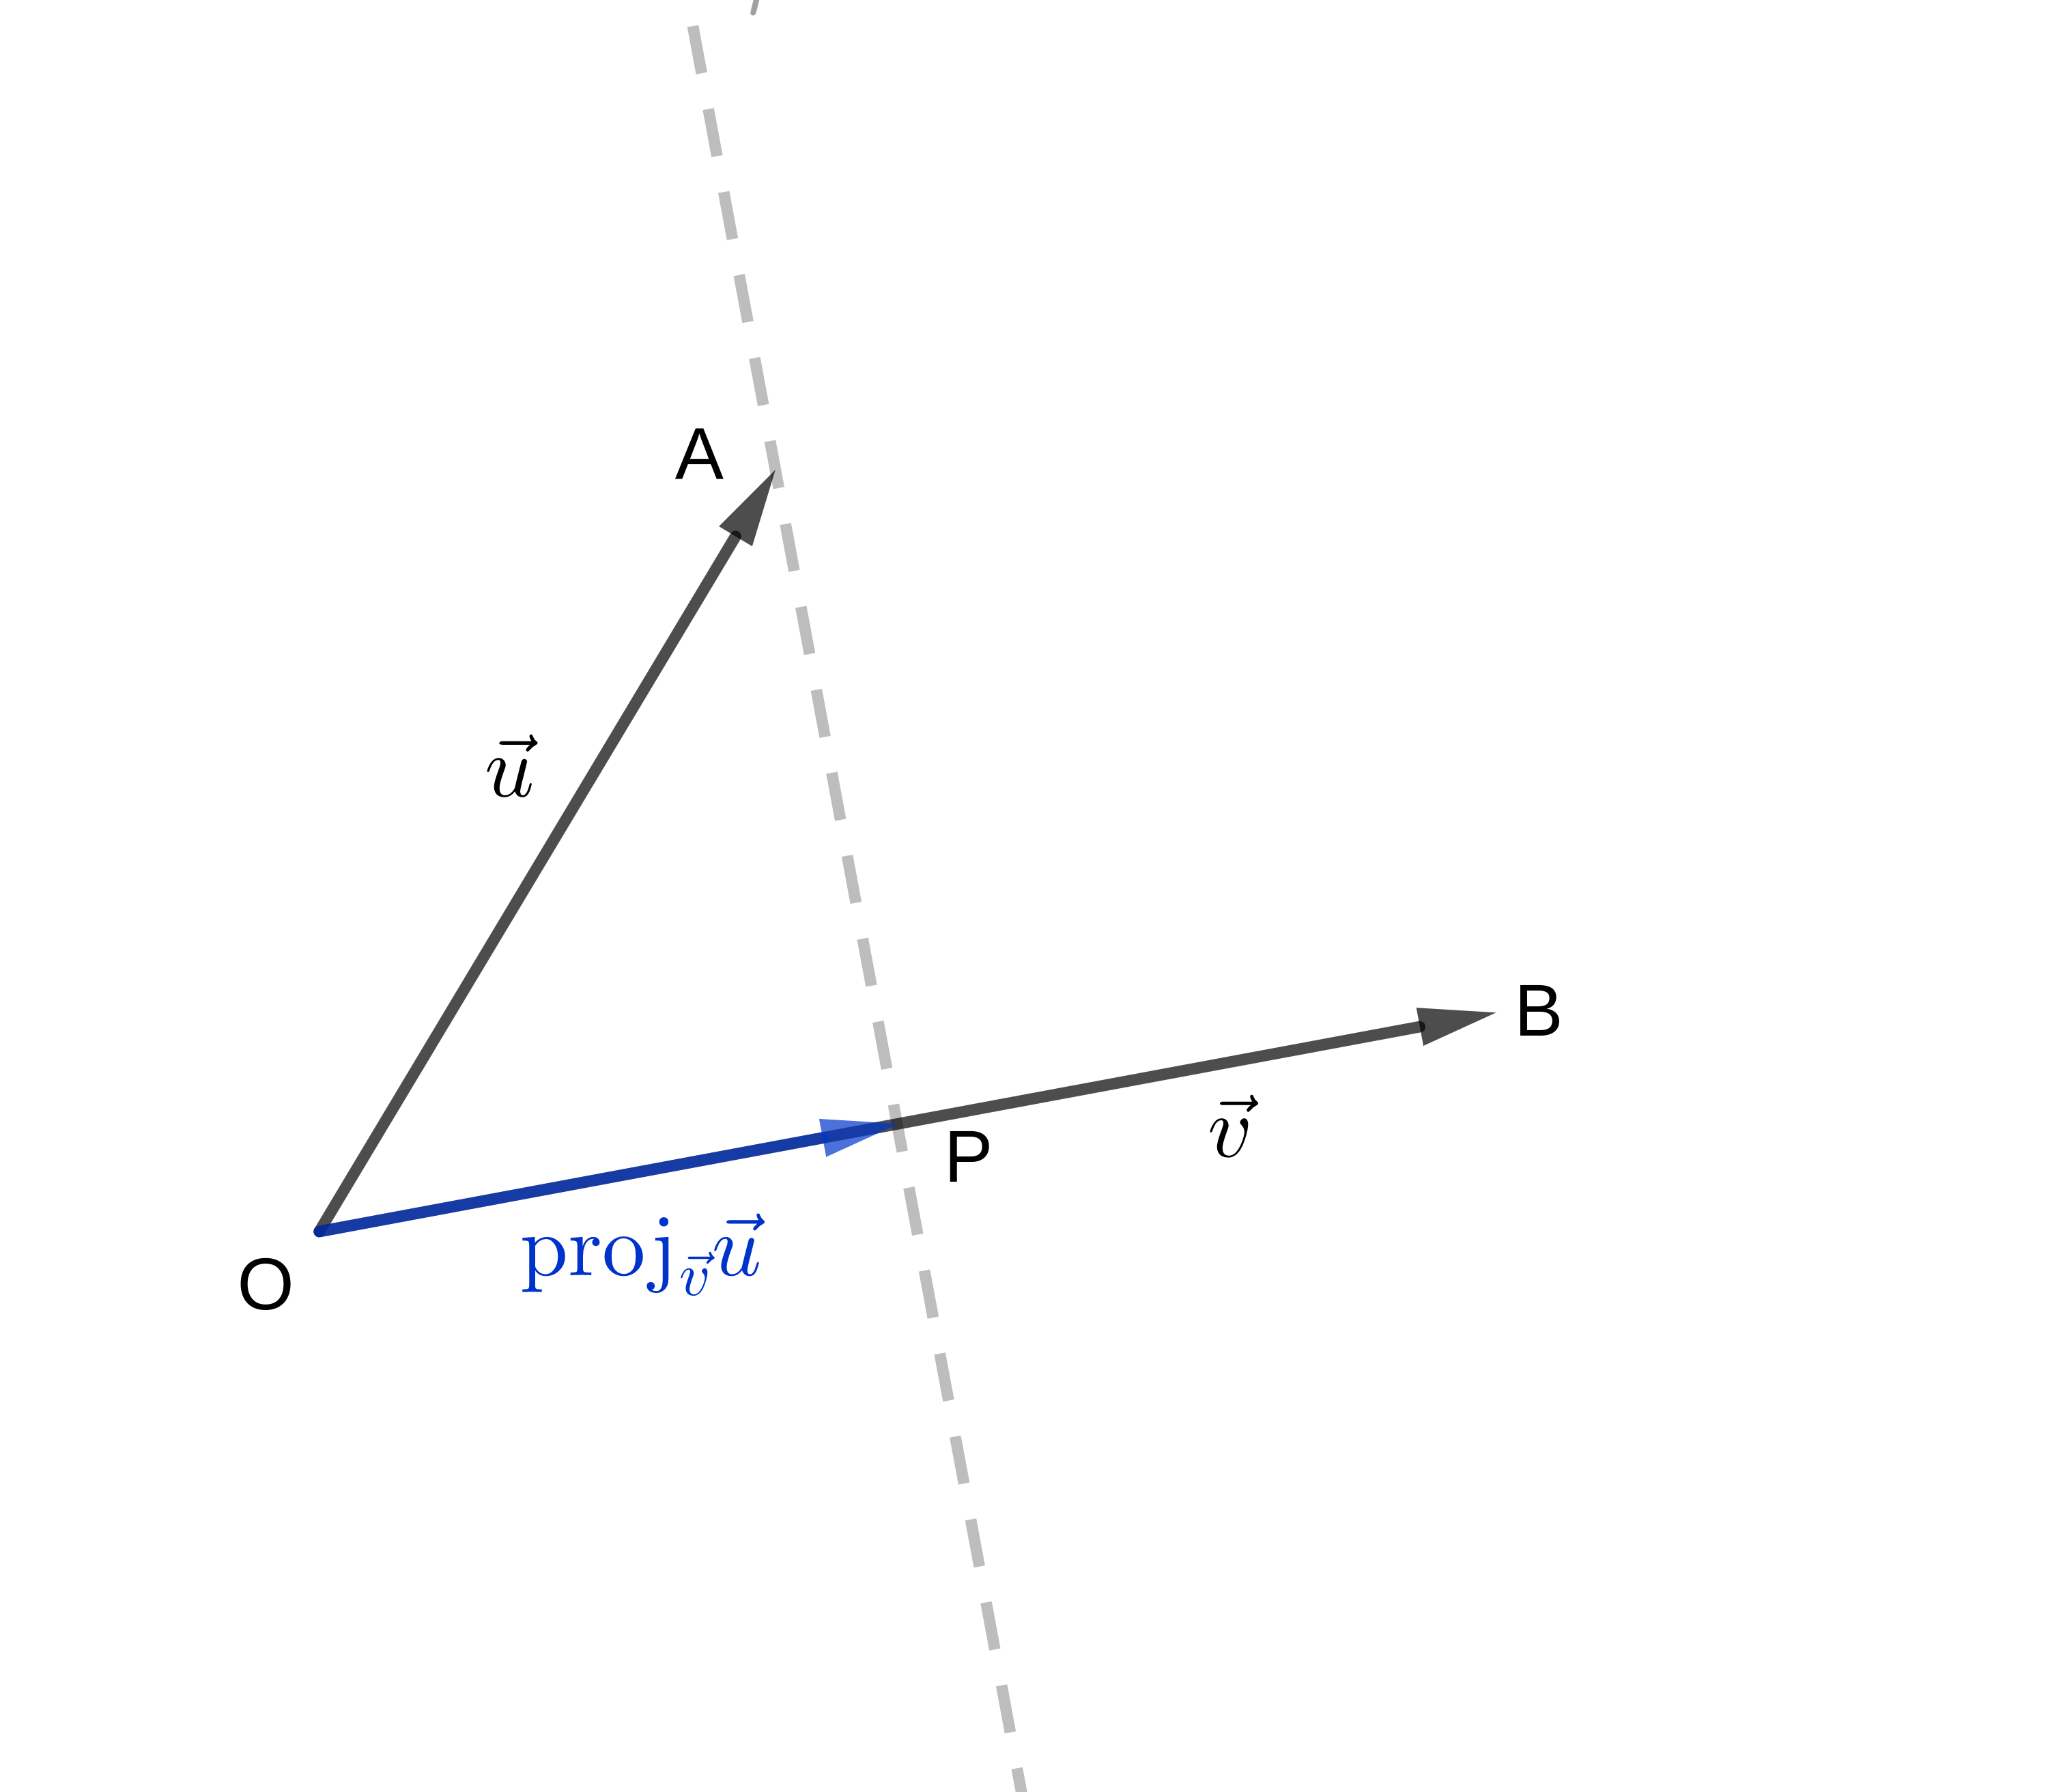
\includegraphics[width=0.7\textwidth]{./cap_produtos/dados/fig_proj/fig_proj}
  \caption{Ilustração da definição da projeção ortogonal.}
  \label{fig:proj}
\end{figure}

Da definição, temos que\footnote{$\proj_{\vec{v}}\vec{u}$ é um vetor múltiplo por escalar de $\vec{v}$.}
\begin{equation}
  {\color{blue}\proj_{\vec{v}}\vec{u} = \beta\cdot \vec{v}}
\end{equation}
para algum número real $\beta$. Além disso, temos
\begin{equation}
  \proj_{\vec{v}}\vec{u} = \vec{u} + \overrightarrow{AP}.
\end{equation}
Portanto
\begin{equation}
  \beta\vec{v} = \vec{u} + \overrightarrow{AP}.
\end{equation}
Tomando o produto escalar com $\vec{v}$ em ambos os lados desta equação, obtemos
\begin{align}
  \beta\vec{v}\cdot\vec{v} &= \vec{u}\cdot\vec{v} + \overrightarrow{AP}\cdot\vec{v} \\
  &= \vec{u}\cdot\vec{v},
\end{align}
pois $\overrightarrow{AP}\perp\vec{v}$. Daí, lembrando que $\vec{v}\cdot\vec{v}=|v|^2$, temos
\begin{equation}
  \alpha = \frac{\vec{u}\cdot\vec{v}}{|\vec{v}|^2}
\end{equation}
e concluímos que
\begin{equation}\label{eq:proj}
  {\color{blue}\proj_{\vec{v}}\vec{u} = \frac{\vec{u}\cdot\vec{v}}{|\vec{v}|^2}\vec{v}}.
\end{equation}

\begin{ex}
  Sejam $\vec{u}=(-1,1,-1)$ e $\vec{v}=(2,1,-2)$. Usando a equação \eqref{eq:proj}, obtemos
  \begin{align}
    \proj_{\vec{v}}\vec{u} &= \frac{(-1,1,-1)\cdot(2,1,-2)}{|(2,1,-2)|^2}(2,1,-2)\\
                           &= \frac{-2+1+2}{4+1+4}(2,1,-2)\\
                           &= \left(\frac{2}{9},\frac{1}{9},\frac{-2}{9}\right).
  \end{align}
\end{ex}

\subsection{Exercícios Resolvidos}

\begin{exeresol}
  Determine $x$ tal que a projeção de $\vec{u}=(1,x,x)$ em $\vec{v}=(1,1,0)$ tenha o dobro da norma de $\vec{v}$.
\end{exeresol}
\begin{resol}
  De \eqref{eq:proj}, a projeção de $\vec{u}$ em $\vec{v}$ é
  \begin{gather}
    \proj_{\vec{v}}\vec{u} = \frac{\vec{u}\cdot\vec{v}}{|\vec{v}|^2}\vec{v},\\
    \left|\proj_{\vec{v}}\vec{u}\right| = \left|\frac{\vec{u}\cdot\vec{v}}{|\vec{v}|^2}\right||\vec{v}| \\
    \left|\proj_{\vec{v}}\vec{u}\right| = \left|\frac{\vec{u}\cdot\vec{v}}{|\vec{v}|}\right| \\
      \left|\proj_{\vec{v}}\vec{u}\right| = \frac{|1+x|}{|\vec{v}|}
  \end{gather}
  Queremos que
  \begin{gather}
    |\proj_{\vec{v}}\vec{u}| = 2|\vec{v}|.
  \end{gather}
  Segue que
  \begin{gather}
    \frac{|1+x|}{|\vec{v}|} = 2|\vec{v}|\\
      |1+x| = 2|\vec{v}|^2 \\
      |1+x| = 2\cdot 2 \\
      1+x = -4\quad\text{ou}\quad 1+x=4\\
      x=-5\quad\text{ou}\quad x=3.
  \end{gather}
\end{resol}

\begin{exeresol}
  Verifique que se $\vec{u}\perp\vec{v}$, então $\proj_{\vec{v}}\vec{u}=\vec{0}$. Justifique sua resposta.
\end{exeresol}
\begin{resol}
  Temos que
  \begin{equation}
    \proj_{\vec{v}}\vec{u} = \frac{\vec{u}\cdot\vec{v}}{|\vec{v}|^2}\vec{v}.
  \end{equation}
  Tendo em vista que $\vec{u}\perp\vec{v}$, temos $\vec{u}\cdot\vec{v}=0$. Logo,
  \begin{align}
    \proj_{\vec{v}}\vec{u} &= 0\cdot\vec{v}\\
                           &= \vec{0}.
  \end{align}
\end{resol}

\subsection{Exercícios}

\begin{exer}
  Sejam $\vec{u}=(-1,1,2)$ e $\vec{v}=(1,-2,0)$. Calcule $\proj_{\vec{v}}\vec{u}$.
\end{exer}
\begin{resp}
  $(-3/5, 6/5, 0)$
\end{resp}

\begin{exer}
  Sejam $\vec{u}$ e $\vec{v}$ vetores unitários e seja $\alpha = \pi/6$ o ângulo entre eles. Calcule a norma da projeção ortogonal de $\vec{u}$ na direção de $\vec{v}$.
\end{exer}
\begin{resp}
  $\frac{\sqrt{3}}{2}$
\end{resp}

\begin{exer}
  Determine $x$ tal que $\proj_{\vec{v}}\vec{u}=(1/6, -1/3, 1/6)$, sendo $\vec{u}=(x,1,2)$ e $\vec{v}=(1,-2,1)$.
\end{exer}
\begin{resp}
  $1$
\end{resp}

\begin{exer}
  Verifique se a $\proj_{\vec{v}}\vec{u}$ tem o mesmo sentido de $\vec{v}$ para quaisquer vetores $\vec{u}$ e $\vec{v}$ dados. Justifique sua resposta.
\end{exer}
\begin{resp}
  Falso
\end{resp}

\begin{exer}
  Determine as coordenadas de todos os vetores $\vec{u}$ tais que $\proj_{\vec{v}}\vec{u}=\vec{v}$, sendo que $\vec{v}=(1,0,0)$.
\end{exer}
\begin{resp}
  $(1,u_2,u_3),~u_1,u_2\in\mathbb{R}$
\end{resp}

\section{Produto Vetorial}\label{cap_prodvet_sec_prodvet}
\badgeRevisar

De agora em diante, vamos trabalhar com um base ortonormal $B = (\vec{i}, \vec{j}, \vec{k})$ dita com orientação positiva, i.e. os vetores $\vec{i} = \overrightarrow{OI}$, $\vec{j} = \overrightarrow{OJ}$ e $\vec{k}=\overrightarrow{OK}$ estão dispostos em sentido anti-horário, veja Figura \ref{fig:base_pos}.

\begin{figure}[H]
  \centering
  \includegraphics[width=0.7\textwidth]{./cap_prodvet/dados/fig_base_pos/fig_base_pos}
  \caption{Base ortonormal positiva.}
  \label{fig:base_pos}
\end{figure}

Dados vetores $\vec{u}$ e $\vec{v}$, definimos o produto vetorial de $\vec{u}$ com $\vec{v}$, denotado por $\vec{u}\land\vec{v}$, como o vetor:
\begin{itemize}
\item se $\vec{u}$ e $\vec{v}$ são l.d., então $\vec{u}\land\vec{v} = \vec{0}$.
\item se $\vec{u}$ e $\vec{v}$ são l.i., então
  \begin{itemize}
  \item $|\vec{u}\land\vec{v}| = |\vec{u}||\vec{v}|\sen\alpha$, onde $\alpha$ é o ângulo entre $\vec{u}$ e $\vec{v}$,
  \item $\vec{u}\land\vec{v}$ é ortogonal a $\vec{u}$ e $\vec{v}$, e
  \item $\vec{u}$, $\vec{v}$ e $\vec{u}\land\vec{v}$ formam uma base positiva.
  \end{itemize}
\end{itemize}

\subsection{Interpretação Geométrica}

Sejam dados $\vec{u}$ e $\vec{v}$ l.i.. Estes vetores determinam um paralelogramo, veja Figura \ref{fig:prodvet_interp} (esquerda). Seja, então, $h$ a altura deste paralelogramo tendo $\vec{u}$ como sua base. Logo, a área do paralelogramo é o produto do comprimento da base com sua altura, neste caso
\begin{align}
  |\vec{u}|h &= |\vec{u}||\vec{v}|\sen\alpha\\
             &= |\vec{u}\land\vec{v}|
\end{align}
Ou seja, o produto vetorial $\vec{u}\land\vec{v}$ tem norma igual à área do paralelogramo determinado por $\vec{u}$ e $\vec{v}$.

Ainda, por definição, $\vec{u}\land\vec{v}$ é ortogonal a $\vec{u}$ e $\vec{v}$. Isto nos dá a direção de $\vec{u}\land\vec{v}$. O sentido é, então, determinado pela definição de que $(\vec{u},\vec{v},\vec{u}\land\vec{v})$ é uma base positiva. Veja a Figura \ref{fig:prodvet_interp} (direita).

\begin{figure}[H]
  \centering
  \includegraphics[width=0.7\textwidth]{./cap_prodvet/dados/fig_prodvet_interp/fig_prodvet_interp}
  \caption{Interpretação do produto vetorial.}
  \label{fig:prodvet_interp}
\end{figure}

\subsection{Produto Vetorial por Coordenadas}\label{cap_prodvet_sec_coord}

Dados $\vec{u} = (u_1,u_2,u_3)$ e $\vec{v} = (v_1,v_2,v_3)$ em uma base ortonormal positiva, então
\begin{equation}
  \vec{u}\land\vec{v} =
  \begin{vmatrix}
    u_2 & u_3\\
    v_2 & v_3
  \end{vmatrix}\vec{i} -
  \begin{vmatrix}
    u_1 & u_3\\
    v_1 & v_3
  \end{vmatrix}\vec{j} +
  \begin{vmatrix}
    u_1 & u_2 \\
    v_1 & v_2
  \end{vmatrix}\vec{k}.
\end{equation}

\begin{obs}
  Uma regra mnemônica, é
  \begin{equation}
    \vec{u}\land\vec{v} =
    \begin{vmatrix}
      \vec{i} & \vec{j} & \vec{k} \\
      u_1 & u_2 & u_3 \\
      v_1 & v_2 & v_3
    \end{vmatrix}.
  \end{equation}
\end{obs}

\begin{ex}
  Dados os vetores $\vec{u} = (1,-2,1)$ e $\vec{v} = (0,2,-1)$, temos
  \begin{align}
    \vec{u}\land\vec{v} &=
                          \begin{vmatrix}
                            \vec{i} & \vec{j} & \vec{k} \\
                            u_1 & u_2 & u_3 \\
                            v_1 & v_2 & v_3
                          \end{vmatrix} \\
                        &=
                          \begin{vmatrix}
                            \vec{i} & \vec{j} & \vec{k} \\
                            1       & -2      & 1 \\
                            0       & 2       & -1
                          \end{vmatrix} \\
                        &= 0\vec{i} + \vec{j} + 2\vec{k}\\
                        &= (0,1,2).
  \end{align}
\end{ex}

\subsection{Exercícios Resolvidos}

\begin{exeresol}
  Calcule $\vec{x}$ tal que $(0,2,-1)\land\vec{x}=(-3,-1,-2)$.
\end{exeresol}
\begin{resol}
  Denotando $\vec{x}=(x_1,x_2,x_3)$, temos
  \begin{gather}
    (0,2,-1)\land\vec{x}=(-3,-1,-2)\\
    \begin{vmatrix}
      \vec{i} & \vec{j} & \vec{k} \\
      0 & 2 & -1 \\
      x_1 & x_2 & x_3
    \end{vmatrix} = (-3,-1,-2)\\
    (x_2+2x_3)\vec{i}-x_1\vec{j}-2x_1\vec{k} = \\
    -3\vec{i}-\vec{j}-2\vec{k}
  \end{gather}
  Segue que
  \begin{align*}
    x_2+2x_3 &= -3\\
    -x_1 &= -1\\
    -2x_1 &= -2
  \end{align*}
  Logo, $x_1 = 1$, $x_2=-3-2x_3$ e $x_3$ é arbitrário. Concluímos que $\vec{x} = (1,-3-2x_3,x_3)$ com $x_3\in\mathbb{R}$.
\end{resol}

\begin{exeresol}
  Determine a área do paralelogramo determinado pelos vetores $\vec{u} = (-1, 2, 3)$ e $\vec{v} = (1,-2,1)$.
\end{exeresol}
\begin{resol}
  Tomando representações $\vec{u}=\overrightarrow{OA}$ e $\vec{v}=\overrightarrow{OC}$, temos que $\vec{u}$ e $\vec{v}$ determinam um paralelogramo $OABC$, onde $C$ é tal que $\vec{u}+\vec{v}=\overrightarrow{OB}$\footnote{Veja a regra do paralelogramo na Observação \ref{obs:vetor_regra_do_paralelogramo}.}. Da definição do produto vetorial, temos que
  \begin{equation}
    |\vec{u}\land\vec{v}| = |\vec{u}||\vec{v}|\sen\alpha,
  \end{equation}
  o que é igual a área do paralelogramo $OABC$, onde $\alpha$ é o ângulo entre os vetores $\vec{u}$ e $\vec{v}$. Logo, a área do paralelogramo é
  \begin{gather}
    |\vec{u}\land\vec{v}| =
    \begin{vmatrix}
      \vec{i} & \vec{j} & \vec{k} \\
      -1 & 2 & 3 \\
      1 & -2 & 1
    \end{vmatrix}\\
    |\vec{u}\land\vec{v}| = |(8,4,0)|\\
    |\vec{u}\land\vec{v}| = 4\sqrt{5}
  \end{gather}
\end{resol}

\subsection{Exercícios}

\begin{exer}
  Sejam $\vec{u}=(2,-3,1)$ e $\vec{v}=(1,-2,-1)$. Calcule:
  \begin{enumerate}[a)]
  \item $\vec{u}\land\vec{v}$.
  \item $\vec{v}\land\vec{u}$.
  \item $\vec{v}\land(2\vec{u})$.
  \end{enumerate}
\end{exer}
\begin{resp}
  a)~$(5,3,-1)$; b)~$(-5,-3,1)$; c)~$(-10,-6,2)$
\end{resp}

\begin{exer}
  Sejam $\vec{u}$ e $\vec{v}$ tais que $\vec{u}\land\vec{v}=(2,-1,0)$. Forneça $\vec{v}\land\vec{u}$. Justifique sua resposta.
\end{exer}
\begin{resp}
  $(-2,1,0)$
\end{resp}

\begin{exer}
  Seja $\vec{u}$ um vetor qualquer. Calcule $\vec{u}\land\vec{u}$.
\end{exer}
\begin{resp}
  $0$
\end{resp}

\begin{exer}
  Sejam $\vec{u}$ e $\vec{v}$ tais que $(2\vec{u})\land\vec{v}=(2,-1,0)$. Forneça $\vec{v}\land\vec{u}$. Justifique sua resposta.
\end{exer}
\begin{resp}
  $(-1,1/2,0)$
\end{resp}

\begin{exer}
  Calcule $\vec{x}$ tal que $\vec{x}\land (2,-2,3)=(11,8,2)$.
\end{exer}
\begin{resp}
  $\left(-\frac{2}{3}x_3+\frac{8}{3},\frac{2}{3}x_3-\frac{11}{3},x_3\right), x_3\in\mathbb{R}$
\end{resp}

\begin{exer}
  Seja $B=(\vec{i},\vec{j},\vec{k})$ uma base ortonormal positiva. Calcule:
  \begin{enumerate}[a)]
  \item $\vec{i}\land\vec{j}$
  \item $\vec{j}\land\vec{k}$
  \item $\vec{k}\land\vec{i}$
  \end{enumerate}
\end{exer}
\begin{resp}
  a)~$\vec{k}$; b)~$\vec{i}$; c)~$\vec{j}$
\end{resp}

\section{Propriedades do Produto Vetorial}\label{cap_prodvet_sec_prop}
\badgeRevisar

Nesta seção, discutiremos sobre algumas propriedades do produto vetorial. Para tanto, sejam dados os vetores $\vec{u} = (u_1,u_2,u_3)$, $\vec{v}=(v_1,v_2,v_3)$, $\vec{w}=(w_1,w_2,w_3)$ e o número real $\gamma$.

Da definição do produto vetorial, temos $\vec{u}\perp(\vec{u}\land\vec{v})$ e $\vec{v}\perp(\vec{u}\land\vec{v})$, logo
\begin{equation}
  {\color{blue}\vec{u}\cdot(\vec{u}\land\vec{v}) = 0}
\end{equation}
e
\begin{equation}
  {\color{blue}\vec{v}\cdot(\vec{u}\land\vec{v}) = 0}.
\end{equation}

\begin{ex}
  Sejam $\vec{u}=(1,-1,2)$, $\vec{v}=(2,-1,-2)$. Temos
  \begin{align}
    \vec{u}\land\vec{v} &=
    \begin{vmatrix}
      \vec{i} & \vec{j} & \vec{k} \\
      1 & -1 & 2 \\
      2 & -1 & -2
    \end{vmatrix}\\
              &= (4,6,1)
  \end{align}
  Segue, que
  \begin{align}
    \vec{u}\cdot(\vec{u}\land\vec{v}) &= (1,-1,2)\cdot (4,6,1) \\
                                      &= 4-6+2\\
                                      &= 0.
  \end{align}
\end{ex}

Em relação à multiplicação por escalar, temos
\begin{align}
  {\color{blue}\gamma(\vec{u}\land\vec{v})} &= {\color{red}(\gamma\vec{u})\land\vec{v}} \\
                              &= {\color{cyan}\vec{u}\land(\gamma\vec{v})}.
\end{align}
De fato,
\begin{align}
  {\color{red}(\gamma\vec{u})\land\vec{v}} &=
                                {\color{red}\begin{vmatrix}
                                  \vec{i} & \vec{j} & \vec{k} \\
                                  \gamma u_1 & \gamma u_2 & \gamma u_3\\
                                  v_1 & v_2 & v_3
                                \end{vmatrix}} \\
                              &= {\color{blue}\gamma\begin{vmatrix}
                                  \vec{i} & \vec{j} & \vec{k} \\
                                  u_1 & u_2 & u_3\\
                                  v_1 & v_2 & v_3
                                \end{vmatrix}} = {\color{blue}\gamma(\vec{u}\land\vec{v})}\\
                              &=
                                {\color{cyan}\begin{vmatrix}
                                  \vec{i} & \vec{j} & \vec{k} \\
                                  u_1 & u_2 & u_3\\
                                  \gamma v_1 & \gamma v_2 & \gamma v_3
                                \end{vmatrix}} = {\color{cyan}\vec{u}\land(\gamma\vec{v})}
\end{align}

\begin{ex}
  Sejam $\vec{u}=(1,-1,2)$ e $\vec{v}=(2,-1,-2)$. Temos
  \begin{align}
    {\color{blue}2(\vec{u}\land\vec{v})} &=
    2\begin{vmatrix}
      \vec{i} & \vec{j} & \vec{k} \\
      1 & -1 & 2 \\
      2 & -1 & -2
    \end{vmatrix}\\
                           &= 2(4,6,1)\\
                           &= (8,12,2)
  \end{align}
  \begin{align}
    {\color{red}(2\vec{u})\land\vec{v}} &=
    \begin{vmatrix}
      \vec{i} & \vec{j} & \vec{k} \\
      2 & -2 & 4 \\
      2 & -1 & -2
    \end{vmatrix}\\
                           &= (8,12,2)
  \end{align}
  \begin{align}
    {\color{cyan}\vec{u}\land(2\vec{v})} &=
    \begin{vmatrix}
      \vec{i} & \vec{j} & \vec{k} \\
      1 & -1 & 2 \\
      4 & -2 & -4
    \end{vmatrix}\\
                           &= (8,12,2)
  \end{align}
\end{ex}


Também, vale a {\color{blue}propriedade distributiva com a operação de soma}, i.e.
\begin{equation}
  {\color{blue}\vec{u}\land(\vec{v} + \vec{w}) = \vec{u}\land\vec{v}+\vec{u}\land\vec{w}}.
\end{equation}
De fato, temos
\begin{gather}
  \vec{u}\land(\vec{v}+\vec{w}) \\
  = \begin{vmatrix}
    \vec{i} & \vec{j} & \vec{k} \\
    u_1 & u_2 & u_3 \\
    v_1+w_1 & v_2+w_2 & u_3+w_3
  \end{vmatrix} \\
  = \begin{vmatrix}
    \vec{i} & \vec{j} & \vec{k} \\
    u_1 & u_2 & u_3 \\
    v_1 & v_2 & v_3
  \end{vmatrix}
  +  \begin{vmatrix}
    \vec{i} & \vec{j} & \vec{k} \\
    u_1 & u_2 & u_3 \\
    w_1 & w_2 & w_3
  \end{vmatrix}\\
  = \vec{u}\land\vec{v} + \vec{u}\land\vec{w}.
\end{gather}

\begin{ex}
  Sejam $\vec{u}=(1,-1,2)$, $\vec{v}=(2,-1,-2)$ e $\vec{w}=(0,-1,-1)$. Temos
  \begin{gather}
    \vec{u}\land(\vec{v}+\vec{w}) \\
    = \vec{u}\land \left[(2,-1,-2)+(0,-1,-1)\right]
    = (1,-1,2)\land (2,-2,-3) \\
    = \begin{vmatrix}
      \vec{i} & \vec{j} & \vec{k} \\
      1 & -1 & 2 \\
      2 & -2 & -3
    \end{vmatrix} \\
    = (7,7,0)  
  \end{gather}
  \begin{gather}
    (\vec{u}\land\vec{v}) + (\vec{u}\land\vec{w}) \\
        = \begin{vmatrix}
          \vec{i} & \vec{j} & \vec{k} \\
          1 & -1 & 2 \\
          2 & -1 & -2
        \end{vmatrix} + \begin{vmatrix}
          \vec{i} & \vec{j} & \vec{k} \\
          1 & -1 & 2 \\
          0 & -1 & -1
        \end{vmatrix} \\
        = (4,6,1) + (3,1,-1) \\
        = (7,7,0)
  \end{gather}
\end{ex}

Observamos que o {\color{blue}produto vetorial não é comutativo}, entretanto
\begin{equation}
  {\color{blue}\vec{u}\land\vec{v} = -\vec{v}\land\vec{u}}.
\end{equation}
De fato, temos
\begin{gather}
  \vec{u}\land\vec{v} \\
  = \begin{vmatrix}
    \vec{i} & \vec{j} & \vec{k} \\
    u_1 & u_2 & u_3 \\
    v_1 & v_2 & v_3                                    
  \end{vmatrix}\\
  = -\begin{vmatrix}
    \vec{i} & \vec{j} & \vec{k} \\
    v_1 & v_2 & v_3 \\
    u_1 & u_2 & u_3                                    
  \end{vmatrix}\\
  = -\vec{v}\land\vec{u}.
\end{gather}

\begin{ex}
  Sejam $\vec{u}=(1,-1,2)$ e $\vec{v}=(2,-1,-2)$. Temos
  \begin{align}
    \vec{u}\land\vec{v} \\
    &= \begin{vmatrix}
      \vec{i} & \vec{j} & \vec{k} \\
      1 & -1 & 2 \\
      2 & -1 & -2                                    
    \end{vmatrix} \\
    &= (4,6,1)
  \end{align}
  \begin{align}
    \vec{v}\land\vec{u} \\
    &= \begin{vmatrix}
      \vec{i} & \vec{j} & \vec{k} \\
      2 & -1 & -2 \\
      1 & -1 & 2
    \end{vmatrix} \\
    &= (-4,-6,-1)
  \end{align}
\end{ex}

Também, o {\color{blue}produto vetorial não é associativo} sendo $(\vec{u}\land\vec{v})\land\vec{w}$, em geral, é diferente de $\vec{u}\land(\vec{v}\land\vec{w})$. Com efeito, temos
\begin{align}
  {\color{blue}(\vec{i}\land\vec{i})\land\vec{j}} &= \vec{0},\\
  {\color{blue}\vec{i}\land(\vec{i}\land\vec{j})} &= \vec{i}\land\vec{k} = -\vec{j}.
\end{align}

Por outro lado, suponhamos que $\vec{u}$, $\vec{v}$ e $\vec{w}$ são l.i. e seja $\pi$ um plano determinado por $\vec{u}$ e $\vec{v}$. Então, $\vec{u}\land\vec{v}$ é ortogonal a $\pi$. Como $(\vec{u}\land\vec{v})\land\vec{w}$ é ortogonal a $\vec{u}\land\vec{v}$ e a $\vec{w}$, temos que $(\vec{u}\land\vec{v})\land\vec{w}$ também pertence a $\pi$. Logo, $\vec{u}$, $\vec{v}$ e $(\vec{u}\land\vec{v})\land\vec{w}$ são l.d. e existem $\alpha$ e $\beta$ tais que
\begin{equation}
  {\color{blue}(\vec{u}\land\vec{v})\land\vec{w} = \alpha\vec{u} + \beta\vec{v}}.
\end{equation}
Vamos determinar $\alpha$ e $\beta$. Para tanto, consideremos uma base ortonormal $B = (\vec{i}, \vec{j}, \vec{k})$ tal que $\vec{i}\parallel\vec{u}$ e $\vec{j}\in\pi$. Nesta base, temos
\begin{align}
  \vec{u} &= (u_1,0,0)\\
  \vec{v} &= (v_1,v_2,0)\\
  \vec{w} &= (w_1,w_2,w_3).
\end{align}
Também, temos
\begin{align}
  \vec{u}\land\vec{v} &=
  \begin{vmatrix}
    \vec{i} & \vec{j} & \vec{k} \\
    u_1 & 0 & 0 \\
    v_1 & v_2 & 0
  \end{vmatrix} \\
  &= (0,0,u_1v_2)
\end{align}
e
\begin{align}
  (\vec{u}\land\vec{v})\land\vec{w} &=
                                      \begin{vmatrix}
                                        \vec{i} & \vec{j} & \vec{k} \\
                                        0 & 0 & u_1v_2 \\
                                        w_1 & w_2 & w_3
                                      \end{vmatrix}\\
                                    &= (-u_1v_2w_2,u_1v_2w_1,0).
\end{align}
Daí, temos
\begin{equation}
  \underbrace{(-u_1v_2w_2,u_1v_2w_1,0)}_{(\vec{u}\land\vec{v})\land\vec{w}} = \underbrace{\alpha(u_1,0,0)+\beta(v_1,v_2,0)}_{\alpha\vec{u}+\beta\vec{v}},
\end{equation}
donde
\begin{align}
  \alpha u_1+\beta v_1 &= -u_1v_2w_2,\\
  \beta v_2 &= u_1w_1v_2.  
\end{align}
Resolvendo para $\alpha$ e $\beta$, obtemos
\begin{align}
  \alpha &= -v_1w_1-v_2w_2 = -\vec{v}\cdot\vec{w}\\
  \beta &= \vec{u}\vec{w}.
\end{align}
Portanto, temos
\begin{equation}
  {\color{blue}(\vec{u}\land\vec{v})\land\vec{w} = -(\vec{v}\cdot\vec{w})\vec{u}+(\vec{u}\cdot\vec{w})\vec{v}}.
\end{equation}

Usando as identidades acima, obtemos
\begin{align}\label{eq:prodvet_assoc1}
  \vec{u}\land(\vec{v}\land\vec{w}) &= -(\vec{v}\land\vec{w})\land\vec{u}\\
                                    &= (\vec{w}\cdot\vec{u})\vec{v}-(\vec{v}\cdot\vec{u})\vec{w}\\
                                    &= (\vec{u}\cdot\vec{w})\vec{v}-(\vec{u}\cdot\vec{v})\vec{w}
\end{align}
ou seja,
\begin{equation}
  {\color{blue}\vec{u}\land(\vec{v}\land\vec{w}) = (\vec{u}\cdot\vec{w})\vec{v}-(\vec{u}\cdot\vec{v})\vec{w}}.
\end{equation}

\subsection{Exercícios Resolvidos}

\begin{exeresol}
  Sejam $\vec{u}=(-3,-2,-1)$, $\vec{v}=(0,1,2)$ e $\vec{w}=(-1,0,1)$. Calcule
  \begin{equation}
    (\vec{u}\land\vec{v})\land\vec{w}.
  \end{equation}
\end{exeresol}
\begin{resol}
  Seguindo a identidade \eqref{eq:prodvet_assoc1}, segue
  \begin{gather}
    (\vec{u}\land\vec{v})\land\vec{w} \\
    = -(\vec{v}\cdot\vec{w})\vec{u} + (\vec{u}\cdot\vec{w})\vec{v}\\
    = -(0+0+2)\vec{u} + (3+0-1)\vec{v}\\
    = -2(-3,-2,-1)+2(0,1,2)\\
    = (6,4,2)+(0,2,4)\\
    = (6,6,6)
  \end{gather}
\end{resol}


\begin{exeresol}
  Sejam $\vec{u}=(2,x,1)$, $\vec{v}=(-2,3,1)$ e $\vec{w}=(-3,-1,1)$. Calcule $x$ tal que
  \begin{equation}
    \vec{v}\cdot(\vec{u}\land\vec{w})=-16.
  \end{equation}
\end{exeresol}
\begin{resol}
  Por cálculo direto, temos
  \begin{gather}
    \vec{v}\cdot(\vec{u}\land\vec{w})=-16\\
    \vec{v}\cdot
    \begin{vmatrix}
      \vec{i} & \vec{j} & \vec{k}\\
      2 & x & 1 \\
      -3 & -1 & 1
    \end{vmatrix} = -16 \\
    (-2,3,1)\cdot(x+1,-5,3x-2)=-16\\
    x-19 = -16 \\
    x = 3.
  \end{gather}
\end{resol}

\subsection{Exercícios}

\begin{exer}
  Sejam $\vec{u}=(2,-3,1)$ e $\vec{v}=(3,-2,1)$. Calcule $\vec{u}\cdot(\vec{v}\land\vec{u})$. Se $\vec{w}$ é um vetor qualquer, forneça o valor de $\vec{u}\cdot(\vec{w}\land\vec{u})$. Justifique sua resposta.
\end{exer}
\begin{resp}
  $\vec{u}\cdot(\vec{v}\land\vec{u})=0$; $\vec{u}\cdot(\vec{w}\land\vec{u})=0$
\end{resp}

\begin{exer}
  Sabendo que $\vec{u}\land\vec{v}=(1,1,1)$, calcule $\vec{u}\land(2\vec{v})$.
\end{exer}
\begin{resp}
  $(2,2,2)$
\end{resp}

\begin{exer}
  Sabendo que $\vec{u}\land\vec{v}=(1,1,1)$ e $\vec{u}\land\vec{w}=(-1,-1,-1)$, calcule $\vec{u}\land(\vec{v} + \vec{w})$.
\end{exer}
\begin{resp}
  $(0,0,0)$
\end{resp}

\begin{exer}
  Sendo $\vec{a}=(3,-1,2)$, $\vec{b}=(2,-1,-1)$, calcule $(\vec{a}\cdot\vec{k})(\vec{i}\land\vec{b})$.
\end{exer}
\begin{resp}
  $(0,2,-2)$
\end{resp}

\begin{exer}
  Calcule $\vec{w}\land(\vec{u}\land\vec{v})$, sendo $\vec{u}=(1,-1,2)$, $\vec{v}=(0,-1,1)$ e $\vec{w}=(1,0,-1)$.
\end{exer}
\begin{resp}
  $(-1,0,-1)$
\end{resp}

\section{Produto Misto}\label{cap_prodmisto_sec_defn}
\badgeRevisar

O {\bf produto misto} de três vetores $\vec{u}$, $\vec{v}$ e $\vec{w}$, nesta ordem, é definido por
\begin{equation}
  {\color{blue}[\vec{u},\vec{v},\vec{w}] := \vec{u}\land\vec{v}\cdot\vec{w}}.
\end{equation}

Em coordenadas, temos
\begin{gather}
  [\vec{u},\vec{v},\vec{w}] := \vec{u}\land\vec{v}\cdot\vec{w} \\
  = \begin{vmatrix}
    \vec{i} & \vec{j} & \vec{k} \\
    u_1 & u_2 & u_3 \\
    v_1 & v_2 & v_3
  \end{vmatrix} \cdot \vec{w} \\
  = \left(
    \begin{vmatrix}
      u_2 & u_3\\
      v_2 & v_3
    \end{vmatrix}\vec{i} -
    \begin{vmatrix}
      u_1 & u_3 \\
      v_1 & v_3
    \end{vmatrix}\vec{j}  +
    \begin{vmatrix}
      u_1 & u_2\\
      v_1 & v_2
    \end{vmatrix}\vec{k}\right)\cdot(w_1,w_2,w_3)\\
  = \begin{vmatrix}
    u_2 & u_3\\
    v_2 & v_3
  \end{vmatrix}w_1 -
  \begin{vmatrix}
    u_1 & u_3 \\
    v_1 & v_3
  \end{vmatrix}w_2
  + \begin{vmatrix}
    u_1 & u_2\\
    v_1 & v_2
  \end{vmatrix}w_3\\
  = \begin{vmatrix}
    w_1 & w_2 & w_3 \\
    u_1 & u_2 & u_3 \\
    v_1 & v_2 & v_3
  \end{vmatrix} \\
  = \begin{vmatrix}
    u_1 & u_2 & u_3 \\
    v_1 & v_2 & v_3 \\
    w_1 & w_2 & w_3 
  \end{vmatrix}
\end{gather}
Ou seja, temos
\begin{equation}
  {\color{blue}[\vec{u},\vec{v},\vec{w}] = \begin{vmatrix}
    u_1 & u_2 & u_3 \\
    v_1 & v_2 & v_3 \\
    w_1 & w_2 & w_3 
  \end{vmatrix}}
\end{equation}

\begin{ex}
  Dados os vetores $\vec{u} = (1,-1,0)$, $\vec{v} = (1,0,2)$ e $\vec{w} = (1,-1,1)$, temos
  \begin{align}
    [\vec{u},\vec{v},\vec{w}] &=
                                \begin{vmatrix}
                                  u_1 & u_2 & u_3 \\
                                  v_1 & v_2 & v_3 \\
                                  w_1 & w_2 & w_3       
                                \end{vmatrix} \\
                              &= \begin{vmatrix}
                                1 & -1 & 0 \\
                                1 & 0  & 2 \\
                                1 & -1 & 1       
                              \end{vmatrix} \\
                              &= 1
  \end{align}
\end{ex}

\subsection{Interpretação Geométrica}\label{subsec:pm_ig}

Consideramos uma base positiva $(\vec{u},\vec{v},\vec{w})$, com $\vec{u}=\overrightarrow{AB}$, $\vec{v}=\overrightarrow{AD}$ e $\vec{w}=\overrightarrow{AH}$. Conforme vemos na Figura \ref{fig:pm_ig}, estes vetores determinam um paralelepípedo.

\begin{figure}[H]
  \centering
  \includegraphics[width=0.8\textwidth]{cap_prodmisto/dados/fig_pm_ig/fig_pm_ig}
  \caption{Interpretação geométrica do produto misto.}
  \label{fig:pm_ig}
\end{figure}

A base do paralelepípedo é o paralelogramo $ABCD$ de área $|\vec{u}\land\vec{v}|$. Assim sendo, o \emph{volume do paralelepípedo} é
\begin{equation}\label{eq:pm_aux1}
  V = |\vec{u}\land\vec{v}|\cdot h,
\end{equation}
onde $h$ é a altura do prisma. Por sua vez,
\begin{align}
  h &= \left|\proj_{\vec{u}\land\vec{v}}\vec{w}\right| \\
    &= \left|\frac{\vec{w}\cdot(\vec{u}\land\vec{v})}{|\vec{u}\land\vec{v}|^2}\vec{u}\land\vec{v}\right|\\
    &= \frac{\left|\vec{w}\cdot(\vec{u}\land\vec{v})\right|}{|\vec{u}\land\vec{v}|^2}|\vec{u}\land\vec{v}|\\
    &= \frac{\left|\vec{w}\cdot(\vec{u}\land\vec{v})\right|}{|\vec{u}\land\vec{v}|} 
\end{align}
Logo, retornando a \eqref{eq:pm_aux1}, obtemos
\begin{align}
  V &= |\vec{u}\land\vec{v}|\cdot h\\
    &= |\vec{u}\land\vec{v}|\cdot\frac{\left|\vec{w}\cdot(\vec{u}\land\vec{v})\right|}{|\vec{u}\land\vec{v}|} \\
    &= \left|\vec{w}\cdot(\vec{u}\land\vec{v})\right|\\
    &= \left|\vec{u}\land\vec{v}\cdot\vec{w}\right|.
\end{align}
Ou seja, o \emph{volume do paralelepípedo} formado pelos vetores $\vec{u}$, $\vec{v}$ e $\vec{w}$ é igual a norma do produto misto destes vetores, i.e.
\begin{equation}\label{eq:pm_vp}
  {\color{blue}V = |[\vec{u},\vec{v},\vec{w}]|}.
\end{equation}

\begin{ex}
  Vamos calcular o volume do paralelepípedo determinado pelos vetores $\vec{u}=(1,1,0)$, $\vec{v}=(-1,2,0)$ e $\vec{w}=(0,1,1)$. De \eqref{eq:pm_vp}, temos
  \begin{gather}
    V = |[\vec{u},\vec{v},\vec{w}]| \\
    = \left|
      \begin{vmatrix}
        1 & 1 & 0 \\
        -1 & 2 & 0 \\
        0 & 1 & 1
      \end{vmatrix}
    \right| \\
    = |3| = 3.
  \end{gather}
\end{ex}

\subsection{Propriedades}

Valem as seguintes propriedades:
\begin{enumerate}[a)]
\item {\color{blue}$[\vec{u},\vec{v},\vec{w}] = -[\vec{v},\vec{u},\vec{w}]$}

  {\it Demonstração}. De fato, quando permutamos duas linhas em uma matriz, seu determinante troca de sinal.
  
\item {\color{blue}$[\vec{u},\vec{v},\vec{w}] = -[\vec{u},\vec{w},\vec{v}]$}

  {\it Demonstração.} Mesmo argumento da letra a).
  
\item {\color{blue}$[\vec{u},\vec{v},\vec{w}] = [\vec{w},\vec{u},\vec{v}] = [\vec{v},\vec{w},\vec{u}]$}

  {\it Demonstração.} De fato, cada caso acima corresponde a duas consecutivas permutações de linha na matriz associada ao produto misto.
  
\item {\color{blue}$[\vec{u},\vec{v},\vec{w}] = \vec{u}\land\vec{v}\cdot\vec{w} = \vec{u}\cdot\vec{v}\land\vec{w}$}

  {\it Demonstração.} Isto segue de c), i.e.
  \begin{align}
    [\vec{u},\vec{v},\vec{w}] &= [\vec{v},\vec{w},\vec{u}] \\
    \vec{u}\land\vec{v}\cdot\vec{w} &= \vec{v}\land\vec{w}\cdot\vec{u}\\
                              &= \vec{u}\cdot\vec{v}\land\vec{w}.
  \end{align}
  
\item {\color{blue}$[\alpha\vec{u},\vec{v},\vec{w}] = [\vec{u},\alpha\vec{v},\vec{w}]=[\vec{u},\vec{v},\alpha\vec{w}] = \alpha[\vec{u},\vec{v},\vec{w}]$}

  {\it Determinação.} De fato, ao multiplicarmos uma linha de uma matriz por um escalar $\alpha$, seu determinante fica multiplicado por $\alpha$.
  
\item {\color{blue}$[\vec{u}+\vec{z},\vec{v},\vec{w}] = [\vec{u},\vec{v},\vec{w}]+[\vec{z},\vec{v},\vec{w}]$}

  {\it Determinante.} Também segue da propriedade análoga do determinante de matrizes.
\end{enumerate}

\begin{ex}
  Sabendo que $[\vec{u},2\vec{w},\vec{v}] = 2$, vamos calcular $[\vec{u},\vec{v},\vec{w}]$. Do item e) acima, temos
  \begin{align}
    2 &= [\vec{u},2\vec{w},\vec{v}] \\
      &= 2[\vec{u},\vec{w},\vec{v}],
  \end{align}
  donde
  \begin{equation}
    [\vec{u},\vec{w},\vec{v}] = 1.
  \end{equation}
  Agora, do item b), temos
  \begin{equation}
    [\vec{u},\vec{w},\vec{v}] = -[\vec{u},\vec{v},\vec{w}].
  \end{equation}
  Ou seja, concluímos que $[\vec{u},\vec{v},\vec{w}] =  -1$.
\end{ex}

Também, temos as seguinte propriedades envolvendo o produto misto:
\begin{enumerate}[a)]
\item Se ${\color{blue}[\vec{u},\vec{v},\vec{w}] = 0}$, então ${\color{blue}(\vec{u},\vec{v},\vec{w})}$ \emph{não é base}.

  {\it Demonstração}. Seja $[\vec{u},\vec{v},\vec{w}]=0$, i.e. $\vec{u}\land\vec{v}\cdot\vec{w}=0$. No caso de um dos vetores serem nulos, então $(\vec{u},\vec{v},\vec{w})$ não é base. Suponhamos, então, que $\vec{u}$, $\vec{v}$ e $\vec{w}$ são vetores não nulos. Isso implica que $\vec{u}\land\vec{v}=0$ ou $(\vec{u}\land\vec{v})\perp\vec{w}$. No primeiro caso, $\vec{u}$ e $\vec{v}$ são l.d. e, portanto, $(\vec{u},\vec{v},\vec{w})$  não é base. No segundo caso, $(\vec{u}\land\vec{v})\perp\vec{w}$, temos que $\vec{w}$ é coplanar aos vetores $\vec{u}$ e $\vec{v}$, logo $(\vec{u},\vec{v},\vec{w})$ não é base.
  
\item Se ${\color{blue}[\vec{u},\vec{v},\vec{w}] > 0}$, então ${\color{blue}(\vec{u},\vec{v},\vec{w})}$ é uma \emph{base positiva}.

  {\it Demonstração.} Se $[\vec{u},\vec{v},\vec{w}] > 0$, implica que o ângulo entre $\vec{u}\land\vec{v}$ e $\vec{w}$ é agudo, o que garante que $(\vec{u},\vec{v},\vec{w})$ seja uma base positiva.
  
\item Se ${\color{blue}[\vec{u},\vec{v},\vec{w}] < 0}$, então ${\color{blue}(\vec{u},\vec{v},\vec{w})}$ é uma \emph{base negativa}.

  {\it Demonstração.} Se $[\vec{u},\vec{v},\vec{w}] < 0$, implica que o ângulo entre $\vec{u}\land\vec{v}$ e $\vec{w}$ é obtuso, o que garante que $(\vec{u},\vec{v},\vec{w})$ seja uma base negativa.
\end{enumerate}

\subsection{Exercícios Resolvidos}

\begin{exeresol}
  Calcule a área do paralelogramo determinado pelos vetores $\vec{v}=(1,0,-2)$, $\vec{w}=(1,-2,1)$ e $\vec{u}=(0,2,1)$.
\end{exeresol}
\begin{resol}
  Da Subseção \ref{subsec:pm_ig}, temos que o volume do paralelogramo é
  \begin{equation}
    V = |[\vec{u},\vec{v},\vec{w}]|,
  \end{equation}
  não importando a ordem dos vetores\footnote{A ordem dos vetores não altera o módulo do valor do produto misto.}. Assim sendo, temos
  \begin{gather}
    V = |[\vec{u},\vec{v},\vec{w}]| \\
    = \left|
      \begin{vmatrix}
        0 & 2 & 1 \\
        1 & 0 & -2 \\
        1 & -2 & 1 
      \end{vmatrix}
    \right| \\
    = |-8| = 8.
  \end{gather}
\end{resol}

\begin{exeresol}
  Sejam $\vec{u}$, $\vec{v}$ e $\vec{w}$ vetores dados. Verifique a seguinte afirmação:
  \begin{equation}
    [\vec{u},\vec{v}+\alpha\vec{u}+\beta\vec{w},\vec{w}]=[\vec{u},\vec{v},\vec{w}],
  \end{equation}
  onde $\alpha$ e $\beta$ são quaisquer escalares.
\end{exeresol}
\begin{resol}
  Das propriedades do produto misto\footnote{$[\vec{u},\vec{v}+\vec{z},\vec{w}]=[\vec{u},\vec{v},\vec{w}]+[\vec{u},\vec{z},\vec{w}]$.}, temos
  \begin{gather}
    [\vec{u},\vec{v}+\alpha\vec{u}+\beta\vec{w},\vec{w}] \\
    = [\vec{u},\vec{v},\vec{w}] + [\vec{u},\alpha\vec{u}+\beta\vec{w},\vec{w}].
  \end{gather}
  Agora, observamos que $\alpha\vec{u}+\beta\vec{w}$ é combinação linear de $\vec{u}$ e $\vec{v}$, logo $(\vec{u}, \alpha\vec{u}+\beta\vec{w}, \vec{w})$ é l.d. e, portanto,
  \begin{equation}
    [\vec{u},\alpha\vec{u}+\beta\vec{w},\vec{w}] = 0.
  \end{equation}
  Concluímos que
  \begin{equation}
  [\vec{u},\vec{v}+\alpha\vec{u}+\beta\vec{w},\vec{w}]=[\vec{u},\vec{v},\vec{w}].  
  \end{equation}
\end{resol}


\subsection{Exercícios}

\begin{exer}
  Calcule $[\vec{u},\vec{v},\vec{w}]$ sendo $\vec{u}=(-1,0,1)$, $\vec{v}=(1,3,0)$ e $\vec{w}=(1,-2,-1)$.
\end{exer}
\begin{resp}
  -2
\end{resp}

\begin{exer}
  Sejam $\vec{a}=(0,0,2)$, $\vec{d}=(-1,1,1)$ e $\vec{e}=(1,1,1)$. Calcule $[\vec{d},\vec{a},\vec{e}]$.
\end{exer}
\begin{resp}
  $4$
\end{resp}

\begin{exer}
  Sendo $[\vec{u},\vec{v},\vec{w}]=2$, calcule $[2\vec{u},-3\vec{v},\vec{w}]$.
\end{exer}
\begin{resp}
  $-12$
\end{resp}

\begin{exer}
  Sendo $[\vec{u},\vec{v},\vec{w}]=2$, calcule $[2\vec{u}-5\vec{w},-3\vec{v},\vec{w}]$.
\end{exer}
\begin{resp}
  $-12$
\end{resp}

\begin{exer}
  Sejam $\vec{u}=(0,x,2)$, $\vec{v}=(-1,1,1)$ e $\vec{w}=(1,1,1)$. Calcule $x$ de forma que $[\vec{u},\vec{v},\vec{w}]=2$.
\end{exer}
\begin{resp}
  $3$
\end{resp}

% 

\chapter{Produto vetorial}\label{cap_prodvet}
\badgeRevisar

De agora em diante, vamos trabalhar com um base ortonormal $B = (\vec{i}, \vec{j}, \vec{k})$ dita com orientação positiva, i.e. os vetores $\vec{i} = \overrightarrow{OI}$, $\vec{j} = \overrightarrow{OJ}$ e $\vec{k}=\overrightarrow{OK}$ estão dispostos em sentido anti-horário, veja Figura \ref{fig:base_pos}.

\begin{figure}[H]
  \centering
  \includegraphics[width=0.7\textwidth]{./cap_prodvet/dados/fig_base_pos/fig_base_pos}
  \caption{Base ortonormal positiva.}
  \label{fig:base_pos}
\end{figure}

\section{Definição}\label{cap_prodvet_sec_prodvet}
\badgeRevisar

Dados vetores $\vec{u}$ e $\vec{v}$, definimos o produto vetorial de $\vec{u}$ com $\vec{v}$, denotado por $\vec{u}\land\vec{v}$, como o vetor:
\begin{itemize}
\item se $\vec{u}$ e $\vec{v}$ são l.d., então $\vec{u}\land\vec{v} = \vec{0}$.
\item se $\vec{u}$ e $\vec{v}$ são l.i., então
  \begin{itemize}
  \item $|\vec{u}\land\vec{v}| = |\vec{u}||\vec{v}|\sen\alpha$, onde $\alpha$ é o ângulo entre $\vec{u}$ e $\vec{v}$,
  \item $\vec{u}\land\vec{v}$ é ortogonal a $\vec{u}$ e $\vec{v}$, e
  \item $\vec{u}$, $\vec{v}$ e $\vec{u}\land\vec{v}$ formam uma base positiva.
  \end{itemize}
\end{itemize}

\subsection{Interpretação geométrica}

Sejam dados $\vec{u}$ e $\vec{v}$ l.i.. Estes vetores determinam um paralelogramo, veja Figura \ref{fig:prodvet_interp} (esquerda). Seja, então, $h$ a altura deste paralelogramo tendo $\vec{u}$ como sua base. Logo, a área do paralelogramo é o produto do comprimento da base com sua altura, neste caso
\begin{align}
  |\vec{u}|h &= |\vec{u}||\vec{v}|\sen\alpha\\
             &= |\vec{u}\land\vec{v}|
\end{align}
Ou seja, o produto vetorial $\vec{u}\land\vec{v}$ tem norma igual à área do paralelogramo determinado por $\vec{u}$ e $\vec{v}$.

Ainda, por definição, $\vec{u}\land\vec{v}$ é ortogonal a $\vec{u}$ e $\vec{v}$. Isto nos dá a direção de $\vec{u}\land\vec{v}$. O sentido é, então, determinado pela definição de que $(\vec{u},\vec{v},\vec{u}\land\vec{v})$ é uma base positiva. Veja a Figura \ref{fig:prodvet_interp} (direita).

\begin{figure}[H]
  \centering
  \includegraphics[width=0.7\textwidth]{./cap_prodvet/dados/fig_prodvet_interp/fig_prodvet_interp}
  \caption{Interpretação do produto vetorial.}
  \label{fig:prodvet_interp}
\end{figure}

\subsection{Produto vetorial via coordenadas}\label{cap_prodvet_sec_coord}

Dados $\vec{u} = (u_1,u_2,u_3)$ e $\vec{v} = (v_1,v_2,v_3)$ em uma base ortonormal positiva, então
\begin{equation}
  \vec{u}\land\vec{v} =
  \begin{vmatrix}
    u_2 & u_3\\
    v_2 & v_3
  \end{vmatrix}\vec{i} -
  \begin{vmatrix}
    u_1 & u_3\\
    v_1 & v_3
  \end{vmatrix}\vec{j} +
  \begin{vmatrix}
    u_1 & u_2 \\
    v_1 & v_2
  \end{vmatrix}\vec{k}.
\end{equation}

\begin{obs}
  Uma regra mnemônica, é
  \begin{equation}
    \vec{u}\land\vec{v} =
    \begin{vmatrix}
      \vec{i} & \vec{j} & \vec{k} \\
      u_1 & u_2 & u_3 \\
      v_1 & v_2 & v_3
    \end{vmatrix}.
  \end{equation}
\end{obs}

\begin{ex}
  Dados os vetores $\vec{u} = (1,-2,1)$ e $\vec{v} = (0,2,-1)$, temos
  \begin{align}
    \vec{u}\land\vec{v} &=
                          \begin{vmatrix}
                            \vec{i} & \vec{j} & \vec{k} \\
                            u_1 & u_2 & u_3 \\
                            v_1 & v_2 & v_3
                          \end{vmatrix} \\
                        &=
                          \begin{vmatrix}
                            \vec{i} & \vec{j} & \vec{k} \\
                            1       & -2      & 1 \\
                            0       & 2       & -1
                          \end{vmatrix} \\
                        &= 0\vec{i} + \vec{j} + 2\vec{k}\\
                        &= (0,1,2).
  \end{align}
\end{ex}

\subsection*{Exercícios resolvidos}

\begin{exeresol}
  Calcule $\vec{x}$ tal que $(0,2,-1)\land\vec{x}=(-3,-1,-2)$.
\end{exeresol}
\begin{resol}
  Denotando $\vec{x}=(x_1,x_2,x_3)$, temos
  \begin{gather}
    (0,2,-1)\land\vec{x}=(-3,-1,-2)\\
    \begin{vmatrix}
      \vec{i} & \vec{j} & \vec{k} \\
      0 & 2 & -1 \\
      x_1 & x_2 & x_3
    \end{vmatrix} = (-3,-1,-2)\\
    (x_2+2x_3)\vec{i}-x_1\vec{j}-2x_1\vec{k} = \\
    -3\vec{i}-\vec{j}-2\vec{k}
  \end{gather}
  Segue que
  \begin{align*}
    x_2+2x_3 &= -3\\
    -x_1 &= -1\\
    -2x_1 &= -2
  \end{align*}
  Logo, $x_1 = 1$, $x_2=-3-2x_3$ e $x_3$ é arbitrário. Concluímos que $\vec{x} = (1,-3-2x_3,x_3)$ com $x_3\in\mathbb{R}$.
\end{resol}

\begin{exeresol}
  Determine a área do paralelogramo determinado pelos vetores $\vec{u} = (-1, 2, 3)$ e $\vec{v} = (1,-2,1)$.
\end{exeresol}
\begin{resol}
  Tomando representações $\vec{u}=\overrightarrow{OA}$ e $\vec{v}=\overrightarrow{OC}$, temos que $\vec{u}$ e $\vec{v}$ determinam um paralelogramo $OABC$, onde $C$ é tal que $\vec{u}+\vec{v}=\overrightarrow{OB}$\footnote{Veja a regra do paralelogramo na Observação \ref{obs:vetor_regra_do_paralelogramo}.}. Da definição do produto vetorial, temos que
  \begin{equation}
    |\vec{u}\land\vec{v}| = |\vec{u}||\vec{v}|\sen\alpha,
  \end{equation}
  o que é igual a área do paralelogramo $OABC$, onde $\alpha$ é o ângulo entre os vetores $\vec{u}$ e $\vec{v}$. Logo, a área do paralelogramo é
  \begin{gather}
    |\vec{u}\land\vec{v}| =
    \begin{vmatrix}
      \vec{i} & \vec{j} & \vec{k} \\
      -1 & 2 & 3 \\
      1 & -2 & 1
    \end{vmatrix}\\
    |\vec{u}\land\vec{v}| = |(8,4,0)|\\
    |\vec{u}\land\vec{v}| = 4\sqrt{5}
  \end{gather}
\end{resol}

\subsection*{Exercícios}

\begin{exer}
  Sejam $\vec{u}=(2,-3,1)$ e $\vec{v}=(1,-2,-1)$. Calcule:
  \begin{enumerate}[a)]
  \item $\vec{u}\land\vec{v}$.
  \item $\vec{v}\land\vec{u}$.
  \item $\vec{v}\land(2\vec{u})$.
  \end{enumerate}
\end{exer}
\begin{resp}
  a)~$(5,3,-1)$; b)~$(-5,-3,1)$; c)~$(-10,-6,2)$
\end{resp}

\begin{exer}
  Sejam $\vec{u}$ e $\vec{v}$ tais que $\vec{u}\land\vec{v}=(2,-1,0)$. Forneça $\vec{v}\land\vec{u}$. Justifique sua resposta.
\end{exer}
\begin{resp}
  $(-2,1,0)$
\end{resp}

\begin{exer}
  Seja $\vec{u}$ um vetor qualquer. Calcule $\vec{u}\land\vec{u}$.
\end{exer}
\begin{resp}
  $0$
\end{resp}

\begin{exer}
  Sejam $\vec{u}$ e $\vec{v}$ tais que $(2\vec{u})\land\vec{v}=(2,-1,0)$. Forneça $\vec{v}\land\vec{u}$. Justifique sua resposta.
\end{exer}
\begin{resp}
  $(-1,1/2,0)$
\end{resp}

\begin{exer}
  Calcule $\vec{x}$ tal que $\vec{x}\land (2,-2,3)=(11,8,2)$.
\end{exer}
\begin{resp}
  $\left(-\frac{2}{3}x_3+\frac{8}{3},\frac{2}{3}x_3-\frac{11}{3},x_3\right), x_3\in\mathbb{R}$
\end{resp}

\begin{exer}
  Seja $B=(\vec{i},\vec{j},\vec{k})$ uma base ortonormal positiva. Calcule:
  \begin{enumerate}[a)]
  \item $\vec{i}\land\vec{j}$
  \item $\vec{j}\land\vec{k}$
  \item $\vec{k}\land\vec{i}$
  \end{enumerate}
\end{exer}
\begin{resp}
  a)~$\vec{k}$; b)~$\vec{i}$; c)~$\vec{j}$
\end{resp}

\section{Propriedades do produto vetorial}\label{cap_prodvet_sec_prop}
\badgeRevisar

Nesta seção, discutiremos sobre algumas propriedades do produto vetorial. Para tanto, sejam dados os vetores $\vec{u} = (u_1,u_2,u_3)$, $\vec{v}=(v_1,v_2,v_3)$, $\vec{w}=(w_1,w_2,w_3)$ e o número real $\gamma$.

Da definição do produto vetorial, temos $\vec{u}\perp(\vec{u}\land\vec{v})$ e $\vec{v}\perp(\vec{u}\land\vec{v})$, logo
\begin{equation}
  {\color{blue}\vec{u}\cdot(\vec{u}\land\vec{v}) = 0}
\end{equation}
e
\begin{equation}
  {\color{blue}\vec{v}\cdot(\vec{u}\land\vec{v}) = 0}.
\end{equation}

\begin{ex}
  Sejam $\vec{u}=(1,-1,2)$, $\vec{v}=(2,-1,-2)$. Temos
  \begin{align}
    \vec{u}\land\vec{v} &=
    \begin{vmatrix}
      \vec{i} & \vec{j} & \vec{k} \\
      1 & -1 & 2 \\
      2 & -1 & -2
    \end{vmatrix}\\
              &= (4,6,1)
  \end{align}
  Segue, que
  \begin{align}
    \vec{u}\cdot(\vec{u}\land\vec{v}) &= (1,-1,2)\cdot (4,6,1) \\
                                      &= 4-6+2\\
                                      &= 0.
  \end{align}
\end{ex}

Em relação à multiplicação por escalar, temos
\begin{align}
  {\color{blue}\gamma(\vec{u}\land\vec{v})} &= {\color{red}(\gamma\vec{u})\land\vec{v}} \\
                              &= {\color{cyan}\vec{u}\land(\gamma\vec{v})}.
\end{align}
De fato,
\begin{align}
  {\color{red}(\gamma\vec{u})\land\vec{v}} &=
                                {\color{red}\begin{vmatrix}
                                  \vec{i} & \vec{j} & \vec{k} \\
                                  \gamma u_1 & \gamma u_2 & \gamma u_3\\
                                  v_1 & v_2 & v_3
                                \end{vmatrix}} \\
                              &= {\color{blue}\gamma\begin{vmatrix}
                                  \vec{i} & \vec{j} & \vec{k} \\
                                  u_1 & u_2 & u_3\\
                                  v_1 & v_2 & v_3
                                \end{vmatrix}} = {\color{blue}\gamma(\vec{u}\land\vec{v})}\\
                              &=
                                {\color{cyan}\begin{vmatrix}
                                  \vec{i} & \vec{j} & \vec{k} \\
                                  u_1 & u_2 & u_3\\
                                  \gamma v_1 & \gamma v_2 & \gamma v_3
                                \end{vmatrix}} = {\color{cyan}\vec{u}\land(\gamma\vec{v})}
\end{align}

\begin{ex}
  Sejam $\vec{u}=(1,-1,2)$ e $\vec{v}=(2,-1,-2)$. Temos
  \begin{align}
    {\color{blue}2(\vec{u}\land\vec{v})} &=
    2\begin{vmatrix}
      \vec{i} & \vec{j} & \vec{k} \\
      1 & -1 & 2 \\
      2 & -1 & -2
    \end{vmatrix}\\
                           &= 2(4,6,1)\\
                           &= (8,12,2)
  \end{align}
  \begin{align}
    {\color{red}(2\vec{u})\land\vec{v}} &=
    \begin{vmatrix}
      \vec{i} & \vec{j} & \vec{k} \\
      2 & -2 & 4 \\
      2 & -1 & -2
    \end{vmatrix}\\
                           &= (8,12,2)
  \end{align}
  \begin{align}
    {\color{cyan}\vec{u}\land(2\vec{v})} &=
    \begin{vmatrix}
      \vec{i} & \vec{j} & \vec{k} \\
      1 & -1 & 2 \\
      4 & -2 & -4
    \end{vmatrix}\\
                           &= (8,12,2)
  \end{align}
\end{ex}


Também, vale a {\color{blue}propriedade distributiva com a operação de soma}, i.e.
\begin{equation}
  {\color{blue}\vec{u}\land(\vec{v} + \vec{w}) = \vec{u}\land\vec{v}+\vec{u}\land\vec{w}}.
\end{equation}
De fato, temos
\begin{gather}
  \vec{u}\land(\vec{v}+\vec{w}) \\
  = \begin{vmatrix}
    \vec{i} & \vec{j} & \vec{k} \\
    u_1 & u_2 & u_3 \\
    v_1+w_1 & v_2+w_2 & u_3+w_3
  \end{vmatrix} \\
  = \begin{vmatrix}
    \vec{i} & \vec{j} & \vec{k} \\
    u_1 & u_2 & u_3 \\
    v_1 & v_2 & v_3
  \end{vmatrix}
  +  \begin{vmatrix}
    \vec{i} & \vec{j} & \vec{k} \\
    u_1 & u_2 & u_3 \\
    w_1 & w_2 & w_3
  \end{vmatrix}\\
  = \vec{u}\land\vec{v} + \vec{u}\land\vec{w}.
\end{gather}

\begin{ex}
  Sejam $\vec{u}=(1,-1,2)$, $\vec{v}=(2,-1,-2)$ e $\vec{w}=(0,-1,-1)$. Temos
  \begin{gather}
    \vec{u}\land(\vec{v}+\vec{w}) \\
    = \vec{u}\land \left[(2,-1,-2)+(0,-1,-1)\right]
    = (1,-1,2)\land (2,-2,-3) \\
    = \begin{vmatrix}
      \vec{i} & \vec{j} & \vec{k} \\
      1 & -1 & 2 \\
      2 & -2 & -3
    \end{vmatrix} \\
    = (7,7,0)  
  \end{gather}
  \begin{gather}
    (\vec{u}\land\vec{v}) + (\vec{u}\land\vec{w}) \\
        = \begin{vmatrix}
          \vec{i} & \vec{j} & \vec{k} \\
          1 & -1 & 2 \\
          2 & -1 & -2
        \end{vmatrix} + \begin{vmatrix}
          \vec{i} & \vec{j} & \vec{k} \\
          1 & -1 & 2 \\
          0 & -1 & -1
        \end{vmatrix} \\
        = (4,6,1) + (3,1,-1) \\
        = (7,7,0)
  \end{gather}
\end{ex}

Observamos que o {\color{blue}produto vetorial não é comutativo}, entretanto
\begin{equation}
  {\color{blue}\vec{u}\land\vec{v} = -\vec{v}\land\vec{u}}.
\end{equation}
De fato, temos
\begin{gather}
  \vec{u}\land\vec{v} \\
  = \begin{vmatrix}
    \vec{i} & \vec{j} & \vec{k} \\
    u_1 & u_2 & u_3 \\
    v_1 & v_2 & v_3                                    
  \end{vmatrix}\\
  = -\begin{vmatrix}
    \vec{i} & \vec{j} & \vec{k} \\
    v_1 & v_2 & v_3 \\
    u_1 & u_2 & u_3                                    
  \end{vmatrix}\\
  = -\vec{v}\land\vec{u}.
\end{gather}

\begin{ex}
  Sejam $\vec{u}=(1,-1,2)$ e $\vec{v}=(2,-1,-2)$. Temos
  \begin{align}
    \vec{u}\land\vec{v} \\
    &= \begin{vmatrix}
      \vec{i} & \vec{j} & \vec{k} \\
      1 & -1 & 2 \\
      2 & -1 & -2                                    
    \end{vmatrix} \\
    &= (4,6,1)
  \end{align}
  \begin{align}
    \vec{v}\land\vec{u} \\
    &= \begin{vmatrix}
      \vec{i} & \vec{j} & \vec{k} \\
      2 & -1 & -2 \\
      1 & -1 & 2
    \end{vmatrix} \\
    &= (-4,-6,-1)
  \end{align}
\end{ex}

Também, o {\color{blue}produto vetorial não é associativo} sendo $(\vec{u}\land\vec{v})\land\vec{w}$, em geral, é diferente de $\vec{u}\land(\vec{v}\land\vec{w})$. Com efeito, temos
\begin{align}
  {\color{blue}(\vec{i}\land\vec{i})\land\vec{j}} &= \vec{0},\\
  {\color{blue}\vec{i}\land(\vec{i}\land\vec{j})} &= \vec{i}\land\vec{k} = -\vec{j}.
\end{align}

Por outro lado, suponhamos que $\vec{u}$, $\vec{v}$ e $\vec{w}$ são l.i. e seja $\pi$ um plano determinado por $\vec{u}$ e $\vec{v}$. Então, $\vec{u}\land\vec{v}$ é ortogonal a $\pi$. Como $(\vec{u}\land\vec{v})\land\vec{w}$ é ortogonal a $\vec{u}\land\vec{v}$ e a $\vec{w}$, temos que $(\vec{u}\land\vec{v})\land\vec{w}$ também pertence a $\pi$. Logo, $\vec{u}$, $\vec{v}$ e $(\vec{u}\land\vec{v})\land\vec{w}$ são l.d. e existem $\alpha$ e $\beta$ tais que
\begin{equation}
  {\color{blue}(\vec{u}\land\vec{v})\land\vec{w} = \alpha\vec{u} + \beta\vec{v}}.
\end{equation}
Vamos determinar $\alpha$ e $\beta$. Para tanto, consideremos uma base ortonormal $B = (\vec{i}, \vec{j}, \vec{k})$ tal que $\vec{i}\parallel\vec{u}$ e $\vec{j}\in\pi$. Nesta base, temos
\begin{align}
  \vec{u} &= (u_1,0,0)\\
  \vec{v} &= (v_1,v_2,0)\\
  \vec{w} &= (w_1,w_2,w_3).
\end{align}
Também, temos
\begin{align}
  \vec{u}\land\vec{v} &=
  \begin{vmatrix}
    \vec{i} & \vec{j} & \vec{k} \\
    u_1 & 0 & 0 \\
    v_1 & v_2 & 0
  \end{vmatrix} \\
  &= (0,0,u_1v_2)
\end{align}
e
\begin{align}
  (\vec{u}\land\vec{v})\land\vec{w} &=
                                      \begin{vmatrix}
                                        \vec{i} & \vec{j} & \vec{k} \\
                                        0 & 0 & u_1v_2 \\
                                        w_1 & w_2 & w_3
                                      \end{vmatrix}\\
                                    &= (-u_1v_2w_2,u_1v_2w_1,0).
\end{align}
Daí, temos
\begin{equation}
  \underbrace{(-u_1v_2w_2,u_1v_2w_1,0)}_{(\vec{u}\land\vec{v})\land\vec{w}} = \underbrace{\alpha(u_1,0,0)+\beta(v_1,v_2,0)}_{\alpha\vec{u}+\beta\vec{v}},
\end{equation}
donde
\begin{align}
  \alpha u_1+\beta v_1 &= -u_1v_2w_2,\\
  \beta v_2 &= u_1w_1v_2.  
\end{align}
Resolvendo para $\alpha$ e $\beta$, obtemos
\begin{align}
  \alpha &= -v_1w_1-v_2w_2 = -\vec{v}\cdot\vec{w}\\
  \beta &= \vec{u}\vec{w}.
\end{align}
Portanto, temos
\begin{equation}
  {\color{blue}(\vec{u}\land\vec{v})\land\vec{w} = -(\vec{v}\cdot\vec{w})\vec{u}+(\vec{u}\cdot\vec{w})\vec{v}}.
\end{equation}

Usando as identidades acima, obtemos
\begin{align}\label{eq:prodvet_assoc1}
  \vec{u}\land(\vec{v}\land\vec{w}) &= -(\vec{v}\land\vec{w})\land\vec{u}\\
                                    &= (\vec{w}\cdot\vec{u})\vec{v}-(\vec{v}\cdot\vec{u})\vec{w}\\
                                    &= (\vec{u}\cdot\vec{w})\vec{v}-(\vec{u}\cdot\vec{v})\vec{w}
\end{align}
ou seja,
\begin{equation}
  {\color{blue}\vec{u}\land(\vec{v}\land\vec{w}) = (\vec{u}\cdot\vec{w})\vec{v}-(\vec{u}\cdot\vec{v})\vec{w}}.
\end{equation}

\subsection*{Exercícios resolvidos}

\begin{exeresol}
  Sejam $\vec{u}=(-3,-2,-1)$, $\vec{v}=(0,1,2)$ e $\vec{w}=(-1,0,1)$. Calcule
  \begin{equation}
    (\vec{u}\land\vec{v})\land\vec{w}.
  \end{equation}
\end{exeresol}
\begin{resol}
  Seguindo a identidade \eqref{eq:prodvet_assoc1}, segue
  \begin{gather}
    (\vec{u}\land\vec{v})\land\vec{w} \\
    = -(\vec{v}\cdot\vec{w})\vec{u} + (\vec{u}\cdot\vec{w})\vec{v}\\
    = -(0+0+2)\vec{u} + (3+0-1)\vec{v}\\
    = -2(-3,-2,-1)+2(0,1,2)\\
    = (6,4,2)+(0,2,4)\\
    = (6,6,6)
  \end{gather}
\end{resol}


\begin{exeresol}
  Sejam $\vec{u}=(2,x,1)$, $\vec{v}=(-2,3,1)$ e $\vec{w}=(-3,-1,1)$. Calcule $x$ tal que
  \begin{equation}
    \vec{v}\cdot(\vec{u}\land\vec{w})=-16.
  \end{equation}
\end{exeresol}
\begin{resol}
  Por cálculo direto, temos
  \begin{gather}
    \vec{v}\cdot(\vec{u}\land\vec{w})=-16\\
    \vec{v}\cdot
    \begin{vmatrix}
      \vec{i} & \vec{j} & \vec{k}\\
      2 & x & 1 \\
      -3 & -1 & 1
    \end{vmatrix} = -16 \\
    (-2,3,1)\cdot(x+1,-5,3x-2)=-16\\
    x-19 = -16 \\
    x = 3.
  \end{gather}
\end{resol}

\subsection*{Exercícios}

\begin{exer}
  Sejam $\vec{u}=(2,-3,1)$ e $\vec{v}=(3,-2,1)$. Calcule $\vec{u}\cdot(\vec{v}\land\vec{u})$. Se $\vec{w}$ é um vetor qualquer, forneça o valor de $\vec{u}\cdot(\vec{w}\land\vec{u})$. Justifique sua resposta.
\end{exer}
\begin{resp}
  $\vec{u}\cdot(\vec{v}\land\vec{u})=0$; $\vec{u}\cdot(\vec{w}\land\vec{u})=0$
\end{resp}

\begin{exer}
  Sabendo que $\vec{u}\land\vec{v}=(1,1,1)$, calcule $\vec{u}\land(2\vec{v})$.
\end{exer}
\begin{resp}
  $(2,2,2)$
\end{resp}

\begin{exer}
  Sabendo que $\vec{u}\land\vec{v}=(1,1,1)$ e $\vec{u}\land\vec{w}=(-1,-1,-1)$, calcule $\vec{u}\land(\vec{v} + \vec{w})$.
\end{exer}
\begin{resp}
  $(0,0,0)$
\end{resp}

\begin{exer}
  Sendo $\vec{a}=(3,-1,2)$, $\vec{b}=(2,-1,-1)$, calcule $(\vec{a}\cdot\vec{k})(\vec{i}\land\vec{b})$.
\end{exer}
\begin{resp}
  $(0,2,-2)$
\end{resp}

\begin{exer}
  Calcule $\vec{w}\land(\vec{u}\land\vec{v})$, sendo $\vec{u}=(1,-1,2)$, $\vec{v}=(0,-1,1)$ e $\vec{w}=(1,0,-1)$.
\end{exer}
\begin{resp}
  $(-1,0,-1)$
\end{resp}

% 

\chapter{Produto misto}\label{cap_prodmisto}
\badgeRevisar

\section{Produto Misto}\label{cap_prodmisto_sec_defn}
\badgeRevisar

O {\bf produto misto} de três vetores $\vec{u}$, $\vec{v}$ e $\vec{w}$, nesta ordem, é definido por
\begin{equation}
  {\color{blue}[\vec{u},\vec{v},\vec{w}] := \vec{u}\land\vec{v}\cdot\vec{w}}.
\end{equation}

Em coordenadas, temos
\begin{gather}
  [\vec{u},\vec{v},\vec{w}] := \vec{u}\land\vec{v}\cdot\vec{w} \\
  = \begin{vmatrix}
    \vec{i} & \vec{j} & \vec{k} \\
    u_1 & u_2 & u_3 \\
    v_1 & v_2 & v_3
  \end{vmatrix} \cdot \vec{w} \\
  = \left(
    \begin{vmatrix}
      u_2 & u_3\\
      v_2 & v_3
    \end{vmatrix}\vec{i} -
    \begin{vmatrix}
      u_1 & u_3 \\
      v_1 & v_3
    \end{vmatrix}\vec{j}  +
    \begin{vmatrix}
      u_1 & u_2\\
      v_1 & v_2
    \end{vmatrix}\vec{k}\right)\cdot(w_1,w_2,w_3)\\
  = \begin{vmatrix}
    u_2 & u_3\\
    v_2 & v_3
  \end{vmatrix}w_1 -
  \begin{vmatrix}
    u_1 & u_3 \\
    v_1 & v_3
  \end{vmatrix}w_2
  + \begin{vmatrix}
    u_1 & u_2\\
    v_1 & v_2
  \end{vmatrix}w_3\\
  = \begin{vmatrix}
    w_1 & w_2 & w_3 \\
    u_1 & u_2 & u_3 \\
    v_1 & v_2 & v_3
  \end{vmatrix} \\
  = \begin{vmatrix}
    u_1 & u_2 & u_3 \\
    v_1 & v_2 & v_3 \\
    w_1 & w_2 & w_3 
  \end{vmatrix}
\end{gather}
Ou seja, temos
\begin{equation}
  {\color{blue}[\vec{u},\vec{v},\vec{w}] = \begin{vmatrix}
    u_1 & u_2 & u_3 \\
    v_1 & v_2 & v_3 \\
    w_1 & w_2 & w_3 
  \end{vmatrix}}
\end{equation}

\begin{ex}
  Dados os vetores $\vec{u} = (1,-1,0)$, $\vec{v} = (1,0,2)$ e $\vec{w} = (1,-1,1)$, temos
  \begin{align}
    [\vec{u},\vec{v},\vec{w}] &=
                                \begin{vmatrix}
                                  u_1 & u_2 & u_3 \\
                                  v_1 & v_2 & v_3 \\
                                  w_1 & w_2 & w_3       
                                \end{vmatrix} \\
                              &= \begin{vmatrix}
                                1 & -1 & 0 \\
                                1 & 0  & 2 \\
                                1 & -1 & 1       
                              \end{vmatrix} \\
                              &= 1
  \end{align}
\end{ex}

\subsection{Interpretação geométrica}\label{subsec:pm_ig}

Consideramos uma base positiva $(\vec{u},\vec{v},\vec{w})$, com $\vec{u}=\overrightarrow{AB}$, $\vec{v}=\overrightarrow{AD}$ e $\vec{w}=\overrightarrow{AH}$. Conforme vemos na Figura \ref{fig:pm_ig}, estes vetores determinam um paralelepípedo.

\begin{figure}[H]
  \centering
  \includegraphics[width=0.8\textwidth]{cap_prodmisto/dados/fig_pm_ig/fig_pm_ig}
  \caption{Interpretação geométrica do produto misto.}
  \label{fig:pm_ig}
\end{figure}

A base do paralelepípedo é o paralelogramo $ABCD$ de área $|\vec{u}\land\vec{v}|$. Assim sendo, o \emph{volume do paralelepípedo} é
\begin{equation}\label{eq:pm_aux1}
  V = |\vec{u}\land\vec{v}|\cdot h,
\end{equation}
onde $h$ é a altura do prisma. Por sua vez,
\begin{align}
  h &= \left|\proj_{\vec{u}\land\vec{v}}\vec{w}\right| \\
    &= \left|\frac{\vec{w}\cdot(\vec{u}\land\vec{v})}{|\vec{u}\land\vec{v}|^2}\vec{u}\land\vec{v}\right|\\
    &= \frac{\left|\vec{w}\cdot(\vec{u}\land\vec{v})\right|}{|\vec{u}\land\vec{v}|^2}|\vec{u}\land\vec{v}|\\
    &= \frac{\left|\vec{w}\cdot(\vec{u}\land\vec{v})\right|}{|\vec{u}\land\vec{v}|} 
\end{align}
Logo, retornando a \eqref{eq:pm_aux1}, obtemos
\begin{align}
  V &= |\vec{u}\land\vec{v}|\cdot h\\
    &= |\vec{u}\land\vec{v}|\cdot\frac{\left|\vec{w}\cdot(\vec{u}\land\vec{v})\right|}{|\vec{u}\land\vec{v}|} \\
    &= \left|\vec{w}\cdot(\vec{u}\land\vec{v})\right|\\
    &= \left|\vec{u}\land\vec{v}\cdot\vec{w}\right|.
\end{align}
Ou seja, o \emph{volume do paralelepípedo} formado pelos vetores $\vec{u}$, $\vec{v}$ e $\vec{w}$ é igual a norma do produto misto destes vetores, i.e.
\begin{equation}\label{eq:pm_vp}
  {\color{blue}V = |[\vec{u},\vec{v},\vec{w}]|}.
\end{equation}

\begin{ex}
  Vamos calcular o volume do paralelepípedo determinado pelos vetores $\vec{u}=(1,1,0)$, $\vec{v}=(-1,2,0)$ e $\vec{w}=(0,1,1)$. De \eqref{eq:pm_vp}, temos
  \begin{gather}
    V = |[\vec{u},\vec{v},\vec{w}]| \\
    = \left|
      \begin{vmatrix}
        1 & 1 & 0 \\
        -1 & 2 & 0 \\
        0 & 1 & 1
      \end{vmatrix}
    \right| \\
    = |3| = 3.
  \end{gather}
\end{ex}

\subsection{Propriedades}

Valem as seguintes propriedades:
\begin{enumerate}[a)]
\item {\color{blue}$[\vec{u},\vec{v},\vec{w}] = -[\vec{v},\vec{u},\vec{w}]$}

  {\it Demonstração}. De fato, quando permutamos duas linhas em uma matriz, seu determinante troca de sinal.
  
\item {\color{blue}$[\vec{u},\vec{v},\vec{w}] = -[\vec{u},\vec{w},\vec{v}]$}

  {\it Demonstração.} Mesmo argumento da letra a).
  
\item {\color{blue}$[\vec{u},\vec{v},\vec{w}] = [\vec{w},\vec{u},\vec{v}] = [\vec{v},\vec{w},\vec{u}]$}

  {\it Demonstração.} De fato, cada caso acima corresponde a duas consecutivas permutações de linha na matriz associada ao produto misto.
  
\item {\color{blue}$[\vec{u},\vec{v},\vec{w}] = \vec{u}\land\vec{v}\cdot\vec{w} = \vec{u}\cdot\vec{v}\land\vec{w}$}

  {\it Demonstração.} Isto segue de c), i.e.
  \begin{align}
    [\vec{u},\vec{v},\vec{w}] &= [\vec{v},\vec{w},\vec{u}] \\
    \vec{u}\land\vec{v}\cdot\vec{w} &= \vec{v}\land\vec{w}\cdot\vec{u}\\
                              &= \vec{u}\cdot\vec{v}\land\vec{w}.
  \end{align}
  
\item {\color{blue}$[\alpha\vec{u},\vec{v},\vec{w}] = [\vec{u},\alpha\vec{v},\vec{w}]=[\vec{u},\vec{v},\alpha\vec{w}] = \alpha[\vec{u},\vec{v},\vec{w}]$}

  {\it Determinação.} De fato, ao multiplicarmos uma linha de uma matriz por um escalar $\alpha$, seu determinante fica multiplicado por $\alpha$.
  
\item {\color{blue}$[\vec{u}+\vec{z},\vec{v},\vec{w}] = [\vec{u},\vec{v},\vec{w}]+[\vec{z},\vec{v},\vec{w}]$}

  {\it Determinante.} Também segue da propriedade análoga do determinante de matrizes.
\end{enumerate}

\begin{ex}
  Sabendo que $[\vec{u},2\vec{w},\vec{v}] = 2$, vamos calcular $[\vec{u},\vec{v},\vec{w}]$. Do item e) acima, temos
  \begin{align}
    2 &= [\vec{u},2\vec{w},\vec{v}] \\
      &= 2[\vec{u},\vec{w},\vec{v}],
  \end{align}
  donde
  \begin{equation}
    [\vec{u},\vec{w},\vec{v}] = 1.
  \end{equation}
  Agora, do item b), temos
  \begin{equation}
    [\vec{u},\vec{w},\vec{v}] = -[\vec{u},\vec{v},\vec{w}].
  \end{equation}
  Ou seja, concluímos que $[\vec{u},\vec{v},\vec{w}] =  -1$.
\end{ex}

Também, temos as seguinte propriedades envolvendo o produto misto:
\begin{enumerate}[a)]
\item Se ${\color{blue}[\vec{u},\vec{v},\vec{w}] = 0}$, então ${\color{blue}(\vec{u},\vec{v},\vec{w})}$ \emph{não é base}.

  {\it Demonstração}. Seja $[\vec{u},\vec{v},\vec{w}]=0$, i.e. $\vec{u}\land\vec{v}\cdot\vec{w}=0$. No caso de um dos vetores serem nulos, então $(\vec{u},\vec{v},\vec{w})$ não é base. Suponhamos, então, que $\vec{u}$, $\vec{v}$ e $\vec{w}$ são vetores não nulos. Isso implica que $\vec{u}\land\vec{v}=0$ ou $(\vec{u}\land\vec{v})\perp\vec{w}$. No primeiro caso, $\vec{u}$ e $\vec{v}$ são l.d. e, portanto, $(\vec{u},\vec{v},\vec{w})$  não é base. No segundo caso, $(\vec{u}\land\vec{v})\perp\vec{w}$, temos que $\vec{w}$ é coplanar aos vetores $\vec{u}$ e $\vec{v}$, logo $(\vec{u},\vec{v},\vec{w})$ não é base.
  
\item Se ${\color{blue}[\vec{u},\vec{v},\vec{w}] > 0}$, então ${\color{blue}(\vec{u},\vec{v},\vec{w})}$ é uma \emph{base positiva}.

  {\it Demonstração.} Se $[\vec{u},\vec{v},\vec{w}] > 0$, implica que o ângulo entre $\vec{u}\land\vec{v}$ e $\vec{w}$ é agudo, o que garante que $(\vec{u},\vec{v},\vec{w})$ seja uma base positiva.
  
\item Se ${\color{blue}[\vec{u},\vec{v},\vec{w}] < 0}$, então ${\color{blue}(\vec{u},\vec{v},\vec{w})}$ é uma \emph{base negativa}.

  {\it Demonstração.} Se $[\vec{u},\vec{v},\vec{w}] < 0$, implica que o ângulo entre $\vec{u}\land\vec{v}$ e $\vec{w}$ é obtuso, o que garante que $(\vec{u},\vec{v},\vec{w})$ seja uma base negativa.
\end{enumerate}

\subsection*{Exercícios resolvidos}

\begin{exeresol}
  Calcule a área do paralelogramo determinado pelos vetores $\vec{v}=(1,0,-2)$, $\vec{w}=(1,-2,1)$ e $\vec{u}=(0,2,1)$.
\end{exeresol}
\begin{resol}
  Da Subseção \ref{subsec:pm_ig}, temos que o volume do paralelogramo é
  \begin{equation}
    V = |[\vec{u},\vec{v},\vec{w}]|,
  \end{equation}
  não importando a ordem dos vetores\footnote{A ordem dos vetores não altera o módulo do valor do produto misto.}. Assim sendo, temos
  \begin{gather}
    V = |[\vec{u},\vec{v},\vec{w}]| \\
    = \left|
      \begin{vmatrix}
        0 & 2 & 1 \\
        1 & 0 & -2 \\
        1 & -2 & 1 
      \end{vmatrix}
    \right| \\
    = |-8| = 8.
  \end{gather}
\end{resol}

\begin{exeresol}
  Sejam $\vec{u}$, $\vec{v}$ e $\vec{w}$ vetores dados. Verifique a seguinte afirmação:
  \begin{equation}
    [\vec{u},\vec{v}+\alpha\vec{u}+\beta\vec{w},\vec{w}]=[\vec{u},\vec{v},\vec{w}],
  \end{equation}
  onde $\alpha$ e $\beta$ são quaisquer escalares.
\end{exeresol}
\begin{resol}
  Das propriedades do produto misto\footnote{$[\vec{u},\vec{v}+\vec{z},\vec{w}]=[\vec{u},\vec{v},\vec{w}]+[\vec{u},\vec{z},\vec{w}]$.}, temos
  \begin{gather}
    [\vec{u},\vec{v}+\alpha\vec{u}+\beta\vec{w},\vec{w}] \\
    = [\vec{u},\vec{v},\vec{w}] + [\vec{u},\alpha\vec{u}+\beta\vec{w},\vec{w}].
  \end{gather}
  Agora, observamos que $\alpha\vec{u}+\beta\vec{w}$ é combinação linear de $\vec{u}$ e $\vec{v}$, logo $(\vec{u}, \alpha\vec{u}+\beta\vec{w}, \vec{w})$ é l.d. e, portanto,
  \begin{equation}
    [\vec{u},\alpha\vec{u}+\beta\vec{w},\vec{w}] = 0.
  \end{equation}
  Concluímos que
  \begin{equation}
  [\vec{u},\vec{v}+\alpha\vec{u}+\beta\vec{w},\vec{w}]=[\vec{u},\vec{v},\vec{w}].  
  \end{equation}
\end{resol}


\subsection*{Exercícios}

\begin{exer}
  Calcule $[\vec{u},\vec{v},\vec{w}]$ sendo $\vec{u}=(-1,0,1)$, $\vec{v}=(1,3,0)$ e $\vec{w}=(1,-2,-1)$.
\end{exer}
\begin{resp}
  -2
\end{resp}

\begin{exer}
  Sejam $\vec{a}=(0,0,2)$, $\vec{d}=(-1,1,1)$ e $\vec{e}=(1,1,1)$. Calcule $[\vec{d},\vec{a},\vec{e}]$.
\end{exer}
\begin{resp}
  $4$
\end{resp}

\begin{exer}
  Sendo $[\vec{u},\vec{v},\vec{w}]=2$, calcule $[2\vec{u},-3\vec{v},\vec{w}]$.
\end{exer}
\begin{resp}
  $-12$
\end{resp}

\begin{exer}
  Sendo $[\vec{u},\vec{v},\vec{w}]=2$, calcule $[2\vec{u}-5\vec{w},-3\vec{v},\vec{w}]$.
\end{exer}
\begin{resp}
  $-12$
\end{resp}

\begin{exer}
  Sejam $\vec{u}=(0,x,2)$, $\vec{v}=(-1,1,1)$ e $\vec{w}=(1,1,1)$. Calcule $x$ de forma que $[\vec{u},\vec{v},\vec{w}]=2$.
\end{exer}
\begin{resp}
  $3$
\end{resp}


% endnotes
\ifishtml
\clearpage
\phantomsection
\addcontentsline{toc}{chapter}{Notas}
\theendnotes
\fi

%references
\ifisbook
\clearpage
\phantomsection
\addcontentsline{toc}{chapter}{\bibname}
\fi

\begin{thebibliography}{99}
  \bibitem{Camargo2005a}
    Camargo, I. \& Boulos, P.. Geometria Analítica: um tratamento vetorial, 3. ed., Pearson, 2005. ISBN: \texttt{978-8587918918}

  \bibitem{Gomez2020a}
    Gómez, S.L.. Vetores com aplicações em física, Blucher, 2020. ISBN: \texttt{978-6555060089}

  \bibitem{Maciel2022a}
    Maciel, T.. Vetores e geometria analítica: do seu jeito. Blucher, 2022. ISBN: \texttt{978-6555064001}
  
  \bibitem{Mello2011a}
    Mello, D.A. \& Watanabe, R.G.. Vetores e uma iniciação à geometria analítica, 2. ed., Livraria da Física, 2012. ISBN: \texttt{978-8578611071}.

\end{thebibliography} 

\end{document}
